\documentclass[11pt]{article}
% Degrees of separation -- Supplementary Information.
% Every number is copied from the result write-up of a seeded script in the repository (scripts 01--75),
% from its interim tables, or was computed for this SI by code run on those tables
% (scripts/70_paper_figures.py --si-checks); the source is named in the text or in the table notes.
\usepackage[margin=1in]{geometry}
\usepackage[T1]{fontenc}
\usepackage{lmodern}
\usepackage{amsmath,amssymb}
\usepackage{graphicx}
\usepackage{booktabs}
\usepackage{array}
\usepackage{longtable}
\usepackage{tabularx}
\usepackage{xcolor}
\usepackage[round]{natbib}
\usepackage{url}
\usepackage{etoolbox}
\usepackage{hyperref}
\hypersetup{colorlinks=true,linkcolor=blue!50!black,citecolor=blue!50!black,urlcolor=blue!50!black}

% S-numbering for sections, figures, tables and equations.
\renewcommand{\thesection}{S\arabic{section}}
\renewcommand{\thefigure}{S\arabic{figure}}
\renewcommand{\thetable}{S\arabic{table}}
\renewcommand{\theequation}{S\arabic{equation}}
\renewcommand{\topfraction}{0.92}
\renewcommand{\bottomfraction}{0.8}
\renewcommand{\textfraction}{0.06}
\renewcommand{\floatpagefraction}{0.8}
\setcounter{topnumber}{3}
\setcounter{totalnumber}{4}
\setlength{\LTcapwidth}{\textwidth}
\setlength{\emergencystretch}{3em}
\makeatletter
\renewcommand*\l@subsection{\@dottedtocline{2}{1.5em}{3.3em}}
% Widen the section-number box in the contents so "S10" does not run into its title.
\patchcmd{\l@section}{\setlength\@tempdima{1.5em}}{\setlength\@tempdima{2.3em}}{}{}
\makeatother

\newcommand{\ci}[2]{$[#1,\allowbreak\,#2]$}
\newcommand{\cic}[2]{$\langle #1,\,#2\rangle$}
\newcommand{\scr}[1]{\texttt{scripts/#1}}
\newcommand{\missingfig}[1]{\fbox{\parbox{0.9\linewidth}{\centering\small Figure file \texttt{\detokenize{#1}.png} not found.}}}
% Diagnostic figures are included as produced by their scripts; the file compiles if one is missing.
\newcommand{\sifig}[2][\textwidth]{%
  \IfFileExists{../outputs/figures/#2.png}{\includegraphics[width=#1]{../outputs/figures/#2.png}}{\missingfig{#2}}}
% flows_placement.png is 2,236 x 4,604 px at 140 dpi (1149.9 x 2367.8 bp); it is shown in two parts,
% split at pixel row 1,880 (966.9 bp from the top), which falls in the blank band between panels (d) and (e).
\newcommand{\flowsfig}[2]{%
  \IfFileExists{../outputs/figures/flows_placement.png}{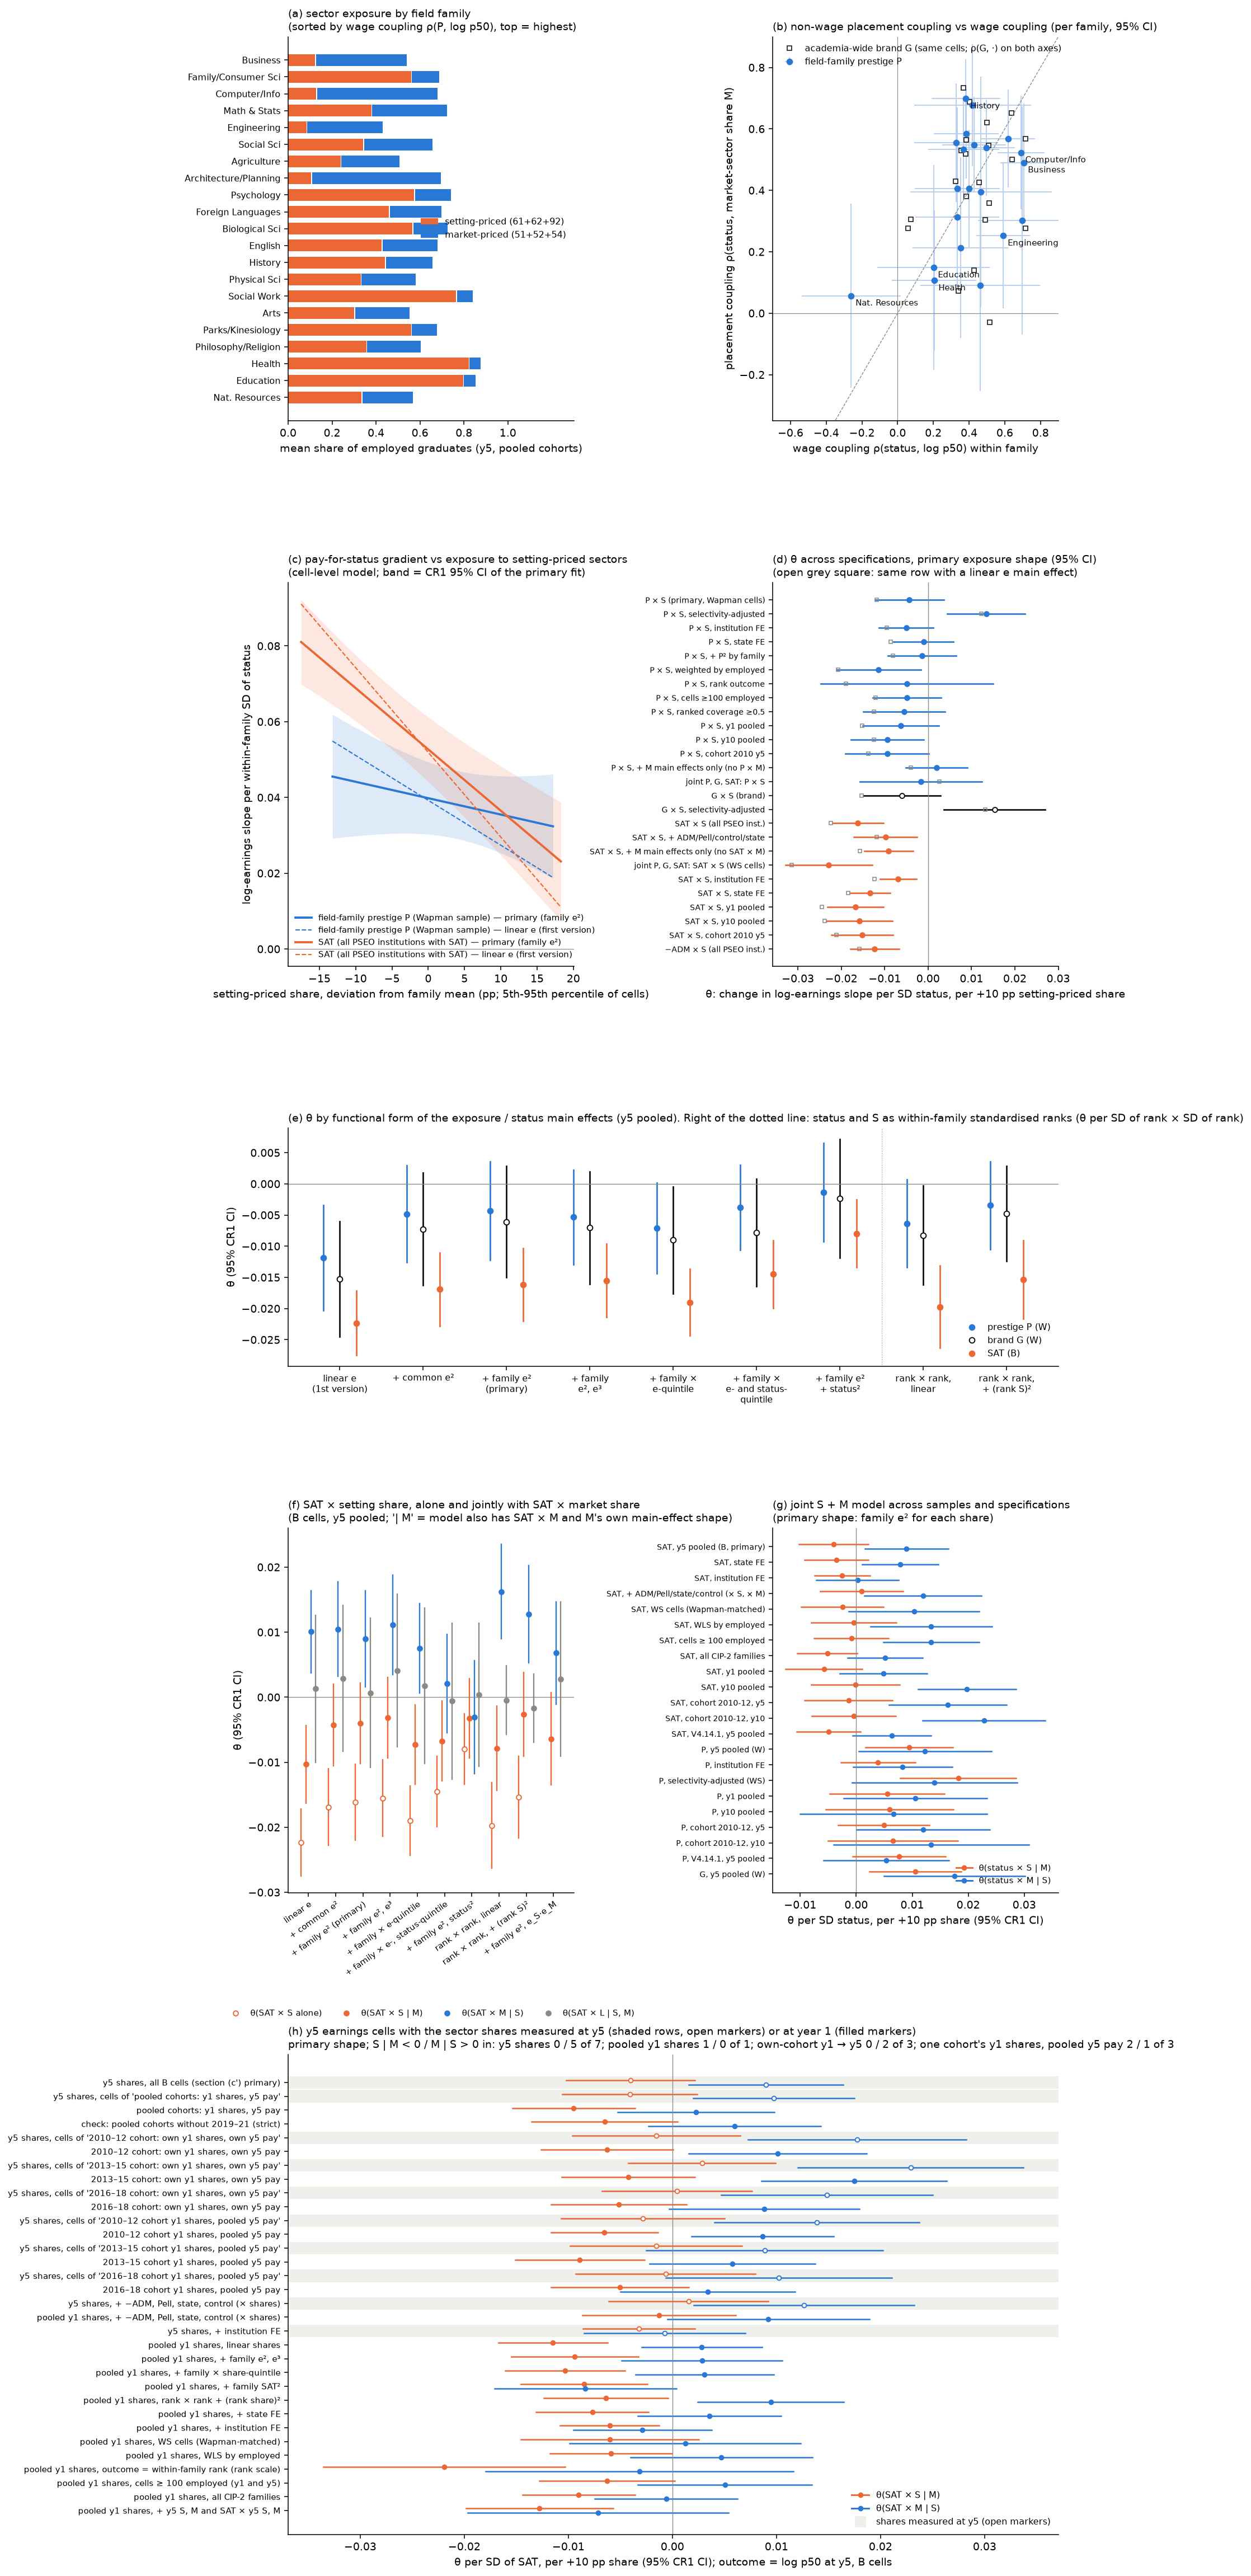
\includegraphics[width=#1,trim=#2,clip]{../outputs/figures/flows_placement.png}}{\missingfig{flows_placement}}}

\title{Supplementary Information for\\[4pt]
\large Degrees of separation: where the academy's hiring order and graduates' pay agree}
\author{Sora Yng}
\date{}

\begin{document}
\maketitle

\noindent This Supplementary Information (SI) gives the methods and the robustness results behind the
main text. Sections S1--S10 follow the order of the analyses: data and crosswalks (S1), prestige measures and the
audits of field prestige (S2), the coupling estimator, its heterogeneity and the reliability of the earnings medians (S3), selectivity
designs, selectivity dated to entry years, field-specific local demand, admission routes and the specification
curve (S4), the UK prior-attainment analysis and its robustness (S5), career time, the graduation-window surface,
entry conditions, graduate study and status loadings (S6), licensing and employer setting (S7), tail outcomes
(S8), the power of the reported nulls and the hypotheses examined (S9) and earnings as a placement measure (S10).
Section S11 states the model of Section~3 of the main text, with its assumptions, derivations, a mapping of the
results to its propositions, and the specification and results of its tests T0--T8. Every analysis is
descriptive. Nothing here identifies value added, selection or employer screening.

\tableofcontents
\bigskip

% =====================================================================================
\section*{Notation and conventions}\addcontentsline{toc}{section}{Notation and conventions}

\paragraph{Variables.} Institution $i$, field $f$. $F_{if}$ is field (department) prestige, minus the
published field rank of \citet{wapman2022quantifying}. $G_i$ is academia-wide prestige, minus the published
rank in the network that pools hires across all fields. $G$ is sometimes read as institutional brand; the SI
uses that word only as a label for $G$, because $G$ also tracks selectivity (Section~\ref{sec:prestige}).
$Y_{if}$ is median earnings. Unless stated otherwise it is the College Scorecard median of Title IV--aided
bachelor's completers four years after completion. Coupling is
\begin{equation}
\rho_f=\operatorname{Spearman}_i\big(F_{if},\,Y_{if}\big),\label{eq:coupling}
\end{equation}
computed across the institutions that teach field $f$. Earlier drafts reported the gap $1-\rho_f$, which
carries the same information; a few legacy slopes below are on that scale and are labelled. $c_F$ and $c_G$
are the couplings of $F$ and of $G$ with $Y$ on the same institutions. In the UK, coupling is the Spearman
correlation across providers within a CAH2 subject between UK academia-wide prestige and LEO median
earnings. $P$ is family prestige, the IPEDS-completions-weighted mean of within-field prestige percentiles
over the ranked fields of a CIP-2 family, and $S$ and $M$ are the shares of a cell's employed graduates in
setting sectors (education, health care and social assistance, public administration) and market sectors
(information, finance and insurance, professional services; Section~\ref{sec:flows}). The ``selectivity
gradient'' of a field is the coupling of institutional selectivity with its earnings, $\rho(\text{SAT},Y)$; it
is a descriptive label, not a mechanism.

\paragraph{Intervals.} Square brackets are 95\% intervals; angle brackets \cic{\cdot}{\cdot} are 95\%
intervals from resampling whole CIP-2 families. The interval type is named where it matters. US
cross-field means of Scorecard statistics use a joint institution bootstrap (institutions resampled once
per draw for every field, so dependence between fields that share institutions is kept). Within-institution
slopes use an institution cluster (pairs) bootstrap. PSEO career-time statistics use the two-way (field,
institution) cluster variance \citep{cameron2011robust}, with the crossed field-by-institution bootstrap beside it
(Section~\ref{sec:intervals}); several later analyses report the two-way variance for Scorecard statistics as
well, and say so. UK statistics resample subjects and then providers within subject (two-stage), or use the
two-way (subject, provider) variance where stated. Tests clustered by state use the wild cluster bootstrap
\citep{cameron2008bootstrap} with Webb weights \citep{webb2023reworking}. Field-level moderators are tested by
field-label permutation and by the CIP-2 family bootstrap. A minimum detectable effect (MDE) is the smallest true
effect with 80\% power in a two-sided 5\% test.

\paragraph{Provenance.} Each number is produced by a seeded script (\scr{NN}, where NN is the script number).
Table~\ref{tab:scriptmap} maps the SI sections to the scripts. At the time of writing, \scr{67}--\scr{69} and
\scr{72}--\scr{75} and the current versions of \scr{65} and \scr{70} are not yet in the public repository; they will
be added in a tagged release. Numbers marked \emph{legacy} come from committed scripts that predate the canonical
specification and were not re-run on it. Numbers marked \emph{SI check} were computed for this SI by
\texttt{scripts/70\_paper\_figures.py --si-checks}, whose header lists them; they include both Scorecard coverage
columns of Table~\ref{tab:coverage} and the count of CIP-4 codes, and they reproduce published values where the two
overlap. The analyses of \scr{65}--\scr{69} and \scr{72}--\scr{75} were added after the main analyses. Each wrote
its tests, samples and reading rules into its docstring before estimation, a timing that is self-reported (the
scripts were not committed before their first runs). Changes made after a first run are labelled exploratory or
post hoc, and the following are listed here: \scr{65} added placebo windows and a $G\times$window-trend version of
its entry-condition test after a development run; \scr{66} added, after its first run, a guard that replaces a
two-way variance below its field part by the larger one-way variance (97 of 680 statistics; no verdict changes), two
sensitivity intervals and the benchmark for the partial forms; \scr{67} added the proportional-mechanism benchmark
of Section~\ref{sec:gradshare} in its first revision; \scr{68}'s pre-set margin for the within-cohort slope is one
third of the raw slope, not of the controlled slope its rule text names, and both readings are reported; \scr{73}
changed its primary correction to the normal-score scale after the per-field reliabilities were computed and before
any test statistic, and an interrupted first build printed its tests once before the reported run; \scr{74}
unified its coding rules after the first estimates (Section~\ref{sec:csadmit}); and \scr{75}'s tests were written after most results had been seen and specified before the analysis, but not
publicly registered: only the SHA-256 digests of their binding texts, checked at run time, record them. The repository also holds
earlier exploratory and withdrawn analyses (\scr{01}--\scr{51}) that are not reported here.

\begin{table}[!tbp]
\centering
\caption{SI sections and the scripts that produce their numbers.}\label{tab:scriptmap}
\footnotesize
\begin{tabular}{@{}>{\raggedright\arraybackslash}p{4.2cm}>{\raggedright\arraybackslash}p{3.4cm}>{\raggedright\arraybackslash}p{7.8cm}@{}}
\toprule
SI section & Scripts & Outputs \\
\midrule
S1 Data and crosswalks & 01, 24, 28, 55, 59, 60, 62, 70 & coverage and matching counts \\
S2 Prestige measures & 56, 62, 75; legacy 09--11, 15--19 & \texttt{data/interim/prestige\_reliability.csv}; T0 and T1 of \scr{75} (\texttt{THEORY\_TESTS\_RESULT.md}) \\
S3 Coupling, heterogeneity, earnings reliability & 02/08, 57, 73 & \texttt{outputs/expanded66\_gap\_map.csv}, \texttt{data/interim/icc\_threelevel.csv}, \texttt{earnings\_reliability*.csv} \\
S4 Selectivity designs & 55, 58, 68, 69, 74 & \texttt{data/interim/selectivity\_fields.csv}, \texttt{selectivity\_deep.csv}, \texttt{era\_selectivity.csv}, \texttt{local\_field\_demand*.csv}, \texttt{cs\_admission\_*.csv} \\
S5 UK LEO & 62, 72 & \texttt{data/interim/uk\_leo\_*.csv}, \texttt{uk\_robustness\_*.csv} \\
S6 Career time & 52, 59, 65, 66, 67, 75; legacy 32 & \texttt{data/interim/career\_time\_coupling.csv}, \texttt{pseo\_refresh.csv}, \texttt{coupling\_dynamics\_results.csv}, \texttt{employer\_learning\_loadings.csv}, \texttt{gradschool\_timing.csv} \\
S7 Licensing and setting & 61, 63, 64; legacy 20, 35c & \texttt{data/interim/licensing\_battery.csv}, \texttt{hierarchical\_power.csv}, \texttt{flows\_placement.csv} \\
S8 Tail outcomes & 60; 59 (quantiles) & \texttt{data/interim/oi\_tail.csv} \\
S9 Power of the nulls & 63 (bounds); 50, 51, 52, 53, 58 & \texttt{data/interim/hierarchical\_power.csv} \\
S10 Placement proxy & 61; legacy 35a, 35b & \texttt{data/interim/er\_axis\_35a\_proxy\_by\_horizon.csv}, \texttt{er\_axis\_35b\_deferral.csv} \\
S11 Model and tests T0--T8 & 75; mapping uses the scripts of S1--S10 & \texttt{THEORY\_TESTS\_RESULT.md} (written by \scr{75}) \\
Main-text figures; SI checks & 70 & \texttt{outputs/figures/paper\_fig1}--\texttt{5}; printed SI-check values (0)--(4) \\
\bottomrule
\end{tabular}
\end{table}

\clearpage
% =====================================================================================
\section{Data and crosswalks}\label{sec:data}

All inputs are public. Table~\ref{tab:sources} lists each source with its release and role. This section
documents how the sources are joined, which institutions and fields enter each analysis, and how coverage
varies along the prestige hierarchy.

{\footnotesize
\begin{longtable}{@{}>{\raggedright\arraybackslash}p{3.0cm}>{\raggedright\arraybackslash}p{5.4cm}>{\raggedright\arraybackslash}p{3.0cm}>{\raggedright\arraybackslash}p{3.6cm}@{}}
\caption{Data sources, releases and roles. Access dates and file checksums are recorded in
\texttt{data/raw/SOURCES.md} of the repository.}\label{tab:sources}\\
\toprule
Source & Release and content used & Role & Sections \\
\midrule
\endfirsthead
\multicolumn{4}{@{}l}{\small Table~\ref{tab:sources} (continued)}\\
\toprule
Source & Release and content used & Role & Sections \\
\midrule
\endhead
\bottomrule
\endfoot
Faculty-hiring data \citep{wapman2022data} & Zenodo v1 (2022-07-29): published SpringRank ordinal ranks at the field and academia-wide levels (\texttt{ranks.csv}); public edge list; 2011--2020 hires & $F$, $G$; reliability & S1--S4, S6--S8 \\
College Scorecard, Field of Study \citep{scorecard} & ``Most recent'' files updated 2026-06-10; 227,980 rows, 178 columns; bachelor's rows (\texttt{CREDLEV} 3); medians at 4 years (canonical), 1 and 5 years (replications) & $Y$ (canonical) & S1, S3, S4, S7, S9 \\
College Scorecard, institution file \citep{scorecard} & ``Most recent'' file, 6,273 institutions; \texttt{SAT\_AVG}, \texttt{ADM\_RATE}, \texttt{PCTPELL}, \texttt{CONTROL}, \texttt{MD\_EARN\_WNE\_P10}, state & selectivity and composition controls & S4, S6, S7 \\
College Scorecard, historical institution files \citep{scorecard} & raw-data archive of 10 June 2026, \texttt{MERGED} files 2001--02 to 2016--17, to 2023--24 for exploratory drift checks (read member by member) & selectivity dated to entry years & S4, S6 \\
PSEO earnings \citep{pseo, pseo2026} & V4.13.0 (2025Q4; 952 institutions, 33 partner jurisdictions) canonical; V4.14.1 (2026Q2; 1,117 institutions, 38 jurisdictions) re-check and the analyses of \scr{65}--\scr{68} and \scr{73}; p25, p50, p75 at y1, y5, y10 by 3-year cohort & replication; career time; quantiles & S1, S3, S6, S10 \\
PSEO Flows \citep{pseo, pseo2026} & institution $\times$ CIP-2 $\times$ NAICS sector counts of employed graduates (V4.13.0; V4.14.1 as a release check) & placement shares $S$, $M$ & S6, S7, S10 \\
DfE, ``Graduate outcomes (LEO): provider level data'', 2022-23 release \citep{dfe_leo_provider} & provider $\times$ CAH2 $\times$ cohort $\times$ YAG 1/3/5 medians (tax years 2015/16--2022/23), all graduates and by prior-attainment band, sex and POLAR4 (marginal breakdowns) & UK earnings & S5, S7 \\
ORCID-derived academic mobility edges \citep{li2026orcid}, built from ORCID public data \citep{orcid}; ROR data dump v2.8 \citep{ror2026data} & 11,987 PhD-to-faculty moves between institutions in Great Britain; ROR identifiers and name variants & UK prestige & S2, S5 \\
Opportunity Insights college tables \citep{chetty2020income} & Mobility Report Card tables 2, 3, 10, 11 (1980--82 birth cohorts; earnings in 2014) & tail outcomes & S8 \\
American Community Survey \citep{census_acs2023_pums} & 2023 1-year public-use microdata, person files and replicate weights & licensed and sector shares by field; graduate-degree shares; field $\times$ state earnings & S4, S6, S7, S9 \\
Survey of Earned Doctorates \citep{ncses_sed_bacc}; IPEDS completions \citep{nces_ipeds} & research doctorates by baccalaureate institution and year; bachelor's completions & doctorate rate per graduate & S6 \\
BLS Local Area Unemployment Statistics \citep{fred_laus} & state $\times$ month unemployment rate, seasonally adjusted & entry conditions & S6 \\
Official university admissions pages & computer-science entry rules, saved with URL, access date and a verbatim quotation (September 2026) & restricted versus open entry & S4 \\
Occupational prestige and underemployment by major & occupational prestige ratings of \citet{hughes2024occupational} \citep{condon2022prestige}; New York Fed college labour-market data \citep{nyfed2026labor} & placement validation (legacy) & S10 \\
\end{longtable}
}

\subsection{Fields, the CIP map and the canonical US sample}\label{sec:fields}

A curated map assigns 80 four-digit CIP codes to 66 fields of the faculty-hiring taxonomy (\scr{28}; count from SI
check (4)). An earlier 54-field map was audited in \scr{24} (legacy): of the 27 taxonomy fields it lacked, 12 were
crosswalk misses and were recovered, 3 are finer splits of existing fields (cell biology, natural resources,
information science), and 12 have no clean bachelor's earnings (graduate-only disciplines, or Scorecard cells
suppressed for small fields). A field's earnings at an institution is the cohort-size-weighted mean of the
medians of its CIP-4 rows at the bachelor's level (weights are the earnings-cohort counts, floored at 1).

Institutions are matched by a normalised name key between the published ranks and the Scorecard institution
names; the Scorecard \texttt{UNITID} then joins the institution file. The match gives 3,527
institution-by-field cells at 227 institutions in the 66 fields, and every cell joins the institution file
(\scr{55}, Method; both counts are reproduced by SI check (4)). 57 fields have at least 8 matched institutions (3,500 cells); they are
used for the heterogeneity, reliability and three-level statistics (\scr{56}, \scr{57}), the cross-source
comparison (Section~\ref{sec:crosssource}) and three rows of the specification curve. 52 fields have at least
15 (3,444 cells; median 48 institutions per field, range 15--173; \scr{55} field table). The name join is
exact after normalisation, so institutions whose Scorecard names carry a campus or city qualifier that the
published ranks omit are lost: of the 50 highest-ranked computer-science departments, 9 are lost this way and 2
more are not matched by the name rules (\scr{74}; Section~\ref{sec:csadmit}). This is the canonical
sample, fixed before the manuscript was drafted, after the analyses had been run: published field ranks,
Scorecard four-year medians, the curated CIP-4 map, and fields with at least 15 institutions.
Section~\ref{sec:speccurve} collects the alternatives.

Among the 227 matched institutions, \texttt{SAT\_AVG} is available for 81.9\%, \texttt{ADM\_RATE} for 96.0\%,
Pell share and institution-wide earnings for 100\%, and the state earnings level for 99.6\% (\scr{55}). 12 of
the 41 institutions without \texttt{SAT\_AVG} are in California, including test-blind campuses, so the ``SAT
sample'' under-represents California public research universities; SAT coverage is 82\%, 82\%, 82\% and 81\%
across academia-wide prestige quartiles, top to bottom. The state earnings level is the leave-one-out mean log
\texttt{MD\_EARN\_WNE\_P10} of the other bachelor's-granting institutions in the state. No public US file
measures the entry attainment of a program's own students: none of the 178 Field-of-Study columns carries SAT
or ACT information, and the 28 SAT/ACT columns of the institution file are institution-wide (\scr{58}).

\subsection{Coverage along the prestige hierarchy}\label{sec:coverage}

Scorecard covers the hierarchy about evenly; PSEO is truncated at the top (Table~\ref{tab:coverage}). The
Scorecard shares are the \scr{01} definition: a ranked institution counts if it has any released bachelor's
earnings cell in the mapped fields. Re-running that definition on the repository's June 2026 Scorecard file
reproduces the published shares exactly (SI check). The PSEO shares use the same definition with a released
five-year pooled-cohort cell; \scr{59} re-ran it on the August 2026 release. Among the 20 most prestigious
institutions, about 18 have no PSEO cell (\scr{01}, legacy).

\begin{table}[!tbp]
\centering
\caption{Coverage of the 371 rows with a published academia-wide rank (369 of them named), by quartile of the
academia-wide rank (quartile sizes 93, 93, 92, 93). Scorecard: any released bachelor's earnings cell in the
mapped fields. PSEO: any released five-year pooled-cohort bachelor's cell in the 30 original fields (the
\scr{01} definition, re-run by \scr{59} on each release); ``aliases'' add hand-checked name matches
(Section~\ref{sec:pseo}).}\label{tab:coverage}
\footnotesize
\begin{tabular}{@{}lcccccc@{}}
\toprule
 & \multicolumn{2}{c}{Scorecard (June 2026 file)} & \multicolumn{4}{c}{PSEO} \\
\cmidrule(lr){2-3}\cmidrule(l){4-7}
Quartile & 30-field map & 66-field map & V4.13.0 & V4.14.1 & + 4 aliases & + 23 aliases \\
\midrule
Q1 (top) & 69 (74.2\%) & 69 (74.2\%) & 20 (21.5\%) & 26 (28.0\%) & 27 (29.0\%) & 29 (31.2\%) \\
Q2 & 60 (64.5\%) & 61 (65.6\%) & 30 (32.3\%) & 34 (36.6\%) & 35 (37.6\%) & 44 (47.3\%) \\
Q3 & 66 (71.7\%) & 66 (71.7\%) & 28 (30.4\%) & 33 (35.9\%) & 35 (38.0\%) & 40 (43.5\%) \\
Q4 (bottom) & 61 (65.6\%) & 61 (65.6\%) & 30 (32.3\%) & 38 (40.9\%) & 38 (40.9\%) & 41 (44.1\%) \\
All & 256 (69.0\%) & 257 (69.3\%) & 108 (29.1\%) & 131 (35.3\%) & 135 (36.4\%) & 154 (41.5\%) \\
\bottomrule
\end{tabular}

\smallskip
\begin{minipage}{0.97\textwidth}\footnotesize
Sources: both Scorecard columns, SI check (4) re-running the \scr{01} definition (the 30-field shares equal the
published 74.2, 64.5, 71.7 and 65.6\%); PSEO
columns, \scr{59} (\texttt{pseo\_refresh.csv}, section \texttt{coverage\_readme\_def}). By the \scr{59} definition (a usable released y5 cell whose field has a published field rank at that
institution; 369 ranked institutions, quartiles 93/92/92/92) the top-quartile counts are 20 (V4.13.0) and 26
(V4.14.1), and the bottom-quartile counts 30 and 35.
\end{minipage}
\end{table}

\subsection{PSEO releases, fixed cohorts and the name-join audit}\label{sec:pseo}

PSEO reports unemployment-insurance wage earnings of graduates by institution, CIP code and three-year
graduation cohort, at one, five and ten years after graduation (y1, y5, y10) \citep{pseo}. The canonical
release is V4.13.0 (2025Q4; 623,084 earnings rows, 952 institutions, 33 partner jurisdictions). The August
2026 release V4.14.1 (2026Q2; 701,293 rows, 1,117 institutions, 38 jurisdictions) is a superset: among
bachelor's institution-by-CIP-4 rows, 134,098 are shared, none exists only in V4.13.0, and of rows released in
both the median changed in 302 of 73,235 at y1, 17 of 67,179 at y5 and 0 of 43,097 at y10 (\scr{59}). The
refresh is a weak test of the career-time result: 71 of the 165 added institutions are in states whose series
start after 2010 (Maryland and New Mexico from 2011, Vermont from 2016), and Tennessee's 24 added
institutions can enter only the 2010 cohort.

Fixed cohorts are the graduation windows 2001--03, 2004--06, 2007--09 and 2010--12. Within each field and
cohort the panel keeps the institutions released at all three horizons (balanced), and a cell needs at least
15 such institutions. The panels have 106 institutions, 142 field-by-cohort cells and 39 fields on V4.13.0,
and 116, 145 and 40 on V4.14.1 (\scr{52}, \scr{59}). Rebuilding the V4.14.1 panel on the V4.13.0
institutions reproduces the V4.13.0 panel exactly.

The project's canonical name join misses institutions in both releases. \scr{59} checks 23 hand-verified
aliases: 4 for added institutions (the three Rutgers campuses and the University of Tennessee, Knoxville) and
19 for institutions already in V4.13.0, among them Stony Brook, Buffalo, Iowa State, Missouri, Albany,
Louisiana State, South Carolina and Hawaii. Joined, the 19 would add 2,244 usable y5 cells to the 14,033 in use
and 1,151 fixed-cohort y10 cells to 6,934. With all 23 aliases the fixed-cohort panel has 137 institutions,
149 cells and 42 fields, and the all-field within-cohort slope is $+0.031$ per year (crossed bootstrap
\ci{+0.018}{+0.042}). No career-time statement changes status in any alias variant
(Section~\ref{sec:refresh}). The aliases are not canonical, because every other script in the analysis uses the canonical join.

\subsection{UK: LEO and the hiring network}\label{sec:ukdata}

The DfE provider-level LEO file reports median earnings by provider (UKPRN), CAH2 subject, academic-year
cohort and year after graduation (YAG 1, 3, 5), for all graduates and separately by prior-attainment band,
sex and POLAR4 quintile (marginal breakdowns only). Suppressed cells are missing, and region-adjusted medians
are suppressed at this grain. Where a provider is published once per region in a cohort-by-YAG cell, only the
region with the most graduates is kept (170 rows dropped). LEO providers are matched to hiring-network
institutions (ROR identifiers) through every ROR name variant and 16 hand-checked aliases: 149 of 171 higher
education institutions match. The primary sample keeps matched institutions with network degree at least 5,
excluding the University of London umbrella node, the Open University and Birkbeck (mostly part-time, mature
students): 134 providers. The cross-section uses the cohorts 2013/14--2016/17 at YAG5 (tax years
2019/20--2022/23), with at least 15 providers per subject-by-cohort cell: 33 subjects. The median share of
graduates included in the earnings figures is 0.727 in these cells (\scr{62}).

\subsection{Opportunity Insights linkage}\label{sec:oidata}

The published academia-wide ranks name 369 institutions. 359 obtain a Scorecard \texttt{UNITID} (293 by
normalised name, 66 by explicit alias), and 340 link to an Opportunity Insights college unit. Dropping units
with insufficient data (31), system groups that pool several campuses (44, including Wisconsin--Madison,
Illinois at Urbana-Champaign and Minnesota), duplicate units, units without outcome rows and unmatched
records leaves 255 single-college units (sample A). Requiring SAT, the 2013 rejection rate, the Barron's 2009
index, parental income and the major mix leaves 242 (sample C, the analysis sample). Where both the Scorecard
route and the name route resolve (279 institutions), they agree on the unit in all 279 (\scr{60}).

\subsection{ACS field-level shares}\label{sec:acs}

Field-level moderators come from the 2023 ACS one-year public-use file (\scr{20}, \scr{63}, \scr{64}). The strict
licensed share is the person-weighted share of a field's full-time employed graduates with positive earnings
whose occupation is a health diagnosing or treating practitioner, lawyer or judge, K-12 teacher, architect or
psychologist (SOC 29-1, 23-1, 25-2, 17-1011, 19-3031). The broad share adds health technicians, accountants
and auditors, licensed engineers and counsellors or social workers (29-2, 13-2011, 17-2, 21-1). Each share is
computed over all degree holders and, as a check, over bachelor's-only holders. The government share is the
share of a field's employed bachelor's-or-higher holders whose employer is a government (class of worker 3--5);
the government-or-non-profit share adds non-profit employers. The ex-ante licensed tag is a hand-coded list of
four fields (nursing, communication disorders, accounting, civil engineering).

\clearpage
% =====================================================================================
\section{Prestige measures}\label{sec:prestige}

The paper uses the published ranks, not a SpringRank rebuilt from the public edge list, because the
public edges reproduce the published field ranks only partly. The published ranks' sampling reliability can
therefore only be bracketed, and every comparison of the couplings $c_F$ and $c_G$ in \scr{56} is reported at
both ends of the bracket, as are the career-time loadings $d_F$ and $d_G$ with $F$ corrected
(\scr{67}; Section~\ref{sec:bfbg}). The horse-race shares (Section~\ref{sec:horse}) and the mirror statistic
(Section~\ref{sec:fieldspecific}) are not reliability-corrected.

\subsection{Published ranks and public-edge SpringRank}\label{sec:springrank}

The public edge list has no edge with fewer than two hires at either the field or the academia-wide level, so
institution pairs linked by a single hire are absent. In the 40 of 57 fields with a published hire count, the
public field edges carry a median 15\% of the field's US-doctorate faculty (self-hires excluded); the
academia-wide network carries 67\%. A median 26\% of ranked institutions per field do not appear in the public
field network at all (computer science: 216 ranked, 130 present). A SpringRank \citep{debacco2018physical}
estimated on all public edges correlates with the published rank at a median Spearman 0.728 across fields
(range 0.32--0.87) and 0.908 for the academia-wide network. These values lie below $\sqrt{\text{rel}}$, the
correlation expected if public-edge sampling noise were the only difference, in 57 of 57 fields (median 0.73
against 0.91; academia-wide 0.908 against 0.979). The published ranks thus carry information the public
edges lack. On the institutions present in the public network, the published $F$ also predicts earnings better
than its public reconstruction: mean $c_F$ is $+0.390$ with the published rank and $+0.323$ with the public
SpringRank ($+0.356$ after disattenuating the reconstruction for its own noise), while mean $c_G$ barely moves
($+0.452$ against $+0.451$). Analyses that rebuild field prestige from public edges therefore lose field
signal.

\subsection{The reliability bracket}\label{sec:bracket}

Split-half reliability is measured on the public edges. Each person on an edge is assigned to one half with
probability one half; SpringRank ($\alpha=10^{-3}$) is estimated on each half; the Spearman correlation of the
halves over the analysis institutions is averaged over 200 seeded splits and stepped up with the
Spearman--Brown formula \citep{spearman1910correlation, brown1910some}. The reliability of $F$ uses the field network on the field's analysis institutions;
the reliability of $G$ uses the academia-wide network on the same institutions, so range restriction is
matched. Two scenarios bracket the published rank:
\begin{itemize}
\item \emph{Lower bound (LB).} The published rank is treated as if estimated from the public edges only. Mean
reliability of $F$ is 0.809 (range 0.56--0.95) and of $G$ 0.993 (range 0.97--1.00) across 57 fields. Because
the published rank uses a superset of these hires, LB is expected to understate its reliability for covered
institutions.
\item \emph{Extrapolated (EXT).} $\text{rel}(m)=m/(m+m_0)$ with $m_0=m_{\text{pub}}(1-\text{rel})/\text{rel}$
from the public split-half, evaluated at the full hire count $m_{\text{pub}}/\text{retention}$. Mean
reliability is 0.960 for $F$ and 0.995 for $G$. Retention (public non-self hires over published US-doctorate
hires net of self-hires) is taken from the published statistics for 40 fields and set to the median (0.150)
for the other 17.
\end{itemize}
Disattenuation divides each coupling by the square root of its prestige reliability; the earnings side is not
corrected, because within a field an earnings reliability rescales $c_F$ and $c_G$ by the same factor and cannot
change their difference's sign.

Field prestige does not detectably out-predict academia-wide prestige at either end of the bracket
(Table~\ref{tab:adv}), although the upper limit under LB ($+0.044$) leaves room for a small advantage. Uncorrected, the mean difference $\text{ADV}=c_F-c_G$ is $-0.049$ \ci{-0.085}{-0.011}
across 57 fields. Under LB it is $-0.005$ \ci{-0.043}{+0.044}; under EXT $-0.042$ \ci{-0.077}{-0.001}. The
across-field mean changes sign only if $F$ is less than $(\bar c_F/\bar c_G)^2=0.795$ as reliable as $G$; the
measured LB ratio averages 0.815, at the break-even point, and the EXT ratio 0.965. No scenario gives an
interval above zero, so none shows $F$ predicting earnings better than $G$. The strict form (``$G$ predicts
better'') does not survive the LB correction. Net of selectivity, $c_F$ and $c_G$ are equal on average
(ADV $+0.00$ \ci{-0.05}{+0.05}, 46 fields; \scr{55}).

\begin{table}[!tbp]
\centering
\caption{Field versus academia-wide prestige as predictors of Scorecard earnings: mean
$\text{ADV}=c_F-c_G$ across fields with 95\% institution-bootstrap intervals (fields held fixed; $B=1000$).
LB and EXT are the reliability scenarios of Section~\ref{sec:bracket}. Source: \scr{56} (rows 1--9) and
\scr{55} (rows 10--11).}\label{tab:adv}
\footnotesize
\begin{tabular}{@{}lcc@{}}
\toprule
Specification & Fields & Mean ADV [95\% CI] \\
\midrule
Uncorrected & 57 & $-0.049$ \ci{-0.085}{-0.011} \\
Uncorrected, fields with $n\ge15$ & 52 & $-0.039$ \ci{-0.070}{-0.009} \\
Lower-bound reliability (LB) & 57 & $-0.005$ \ci{-0.043}{+0.044} \\
LB, fields with $n\ge15$ & 52 & $+0.007$ \ci{-0.025}{+0.050} \\
LB, SpringRank $\alpha=1$ & 57 & $-0.013$ \ci{-0.051}{+0.030} \\
Extrapolated reliability (EXT) & 57 & $-0.042$ \ci{-0.077}{-0.001} \\
EXT, fields with $n\ge15$ & 52 & $-0.032$ \ci{-0.062}{+0.0004} \\
Covered institutions only: uncorrected / LB / EXT & 57 & $-0.063$ / $-0.022$ / $-0.056$ \\
Public-edge reconstructions of $F$ and $G$ (covered institutions) & 57 & $-0.128$ \ci{-0.186}{-0.069} \\
Raw, SAT sample & 47 & $-0.03$ \ci{-0.06}{-0.00} \\
Partial, net of SAT, admission rate, Pell share, control, state level & 46 & $+0.00$ \ci{-0.05}{+0.05} \\
\bottomrule
\end{tabular}

\smallskip
\begin{minipage}{0.97\textwidth}\footnotesize
Covered-institution intervals: uncorrected \ci{-0.106}{-0.021}, LB \ci{-0.068}{+0.030}, EXT
\ci{-0.100}{-0.012}. Uncorrected, ADV is positive in 15 of 57 fields; under LB in 28, under EXT in 17. Per-field
LB intervals are above zero in 3 fields and below in 1.
\end{minipage}
\end{table}

\subsection{Checks on the bracket}\label{sec:bracketchecks}

Three checks support the bracket and one limits it (\scr{56}).
First, classical attenuation holds for the public reconstruction: across 57 fields the mean coupling from
half-edge reconstructions is $+0.301$ observed against $+0.299$ predicted from the full-edge coupling and the
Spearman--Brown reliabilities ($c_G$: $+0.452$ against $+0.450$).
Second, the covered-subset analysis applies reliabilities measured on exactly the institutions in the public
network and gives the same qualitative result (Table~\ref{tab:adv}).
Third, raising the SpringRank regularisation to $\alpha=1$ raises the LB reliability of $F$ (mean 0.839) and
leaves ADV at $-0.013$ \ci{-0.051}{+0.030}.
The limit is the earnings side. The noise-model signal fraction that the reliability flag uses
(Section~\ref{sec:flag}) cannot serve as an earnings reliability: 20 of 57 fields sit at its floor of 0.02, and
in 24 of 57 the observed $\max(|c_F|,|c_G|)$ exceeds $\sqrt{\text{signal fraction}}$, which classical error
does not allow. On the 27 fields with signal fraction at least 0.5, correcting both sides gives the same
pattern as the primary specification (uncorrected $-0.053$ \ci{-0.104}{-0.001}; LB $+0.008$ \ci{-0.043}{+0.087};
EXT $-0.043$ \ci{-0.093}{+0.012}).

The bracket covers sampling noise in the ranks only. Construct differences, for example that $F$ is built from
PhD placement while $Y$ describes bachelor's graduates, are not measurement error and are not corrected.
Narrowing the bracket would need person-level hiring records without the single-pair suppression; more earnings
data would not help, because the unknown is on the prestige side.

\subsection{Does field prestige measure doctoral production?}\label{sec:production}

SpringRank orders departments by the direction of hiring exchange, but departments that produce many PhDs also
place many, so $F$ may partly measure size or research output. \scr{75} audits this on the public field edges and
IPEDS 2023 research doctorates \citep{nces_ipeds}. The audit was specified before it was run but not publicly registered, and it was written after most results had
been seen (Section~\ref{si:theory:tests}). Within fields,
$F$ correlates on average $+0.441$ \ci{+0.387}{+0.497} with log research doctorates, $+0.405$ \ci{+0.366}{+0.444}
with the net export ratio of hires, $+0.664$ with the placement rate and $+0.769$ with the published production rank
(field bootstrap). Replacing $F$ by a degree-corrected rank keeps 0.839 \ci{0.743}{0.936} of mean coupling, and
residualising $F$ on log doctorates and the export ratio keeps 0.598 \ci{0.471}{0.725} (two-way intervals; 56
fields, 2,628 cells); the reading fixed in advance is ``partly production''. That reading bounds the production
share from above, and only through the residualised branch: residualising on the export ratio also removes net
export that valuation itself produces (valued departments export on net under H1), so $1-0.598$ can overstate the
production share. The degree-corrected branch has a separate validity limit: the degree-corrected rank still
carries the export ratio (mean Spearman with it $+0.658$ against $+0.588$ for $F$), so its retained share does not
measure the part of $F$ that is free of volume. Both branches also treat log doctorates and the export ratio as
error-free measures of production, although doctorates come from an IPEDS name match (cells without a match are
dropped) and a matched institution with no doctorates recorded in the field's CIP codes counts as producing none. For $G$, degree correction barely changes mean coupling ($-0.013$
\ci{-0.056}{+0.030}). A within-institution slope with the department's own doctoral output as an added control was not estimated.
A second audit, T1, asks whether one index orders departments both by where their PhDs are hired and by whom they
hire. The ratio of cross-role to within-role split-half agreement is $0.525$ \ci{0.461}{0.583} over 33 fields,
below the threshold of 0.80 set in advance. That threshold ignores boundary effects, which make the two roles
disagree even under one index, so the amended test benchmarks a cross-fitted ratio ($0.658$) against the value
SpringRank's own generative model produces ($0.828$): the difference is $-0.169$ \ci{-0.229}{-0.115}, ``not one
index'', under a calibration of the benchmark adopted after the literal one had degenerated
(Section~\ref{si:theory:tests}). $F$ is therefore read as a net-placement position, not as one belief about the
quality of a department's PhDs.

\subsection{The UK academia-wide hiring hierarchy}\label{sec:ukprestige}

UK prestige $G$ is one SpringRank ($\alpha=10^{-3}$) over all 11,987 PhD-to-faculty moves between institutions
in Great Britain in the ORCID-derived academic mobility edges \citep[version 20260419;][]{li2026orcid}, which are
built from ORCID public records \citep{orcid} with organisations resolved to ROR identifiers (one edge per person,
the first faculty job; 551 institutions keyed by ROR identifier; self-hires dropped; \scr{62}). Institutions are
matched to LEO providers through the name variants of the ROR data dump v2.8 \citep{ror2026data}: 149 of 171 LEO
higher education institutions match, and 134 form the
primary sample (Section~\ref{sec:ukdata}). The median first-faculty-job year of the edges is 2014. Among the 134
primary providers, Russell Group members sit at a mean percentile of 0.859 against 0.430 for other providers
(AUC 0.928; 18 of 23 members in the top quartile). Across 200 person-level bootstrap resamples the median
Spearman correlation with the full-sample ranking is 0.961 (5th percentile 0.944). Across 100 random splits of
persons the median correlation between half-network rankings is 0.850, and 0.919 after the Spearman--Brown
step-up \citep{spearman1910correlation, brown1910some}. $G$ built from post-2000 hires only correlates $+0.994$ with $G$. $G$ correlates $+0.714$ across 133
providers with intake selectivity, the institution's share of graduates who entered with at least 360 UCAS
tariff points.

Field-tagged UK networks are too sparse to serve as the main axis (47 to 504 edges per usable field). On the 16
subjects where the field-tagged axis of \scr{40} is usable, coupling with $G$ exceeds coupling with the
field-tagged axis in 16 of 16 subjects on the same providers and cells (means $+0.639$ against $+0.417$; mean
within-subject Spearman between the two axes $+0.542$). Because the field-tagged axis is far noisier, this shows
that it is no better than $G$, not that field prestige is worse in truth.

These checks are internal. Against an external standard the evidence is indirect: in the US, an academia-wide
ranking rebuilt from the ORCID-derived edges agreed with the census-based published ranks at $\rho=0.74$
(Section~\ref{sec:validation}), so an ORCID-based hierarchy may measure standing less validly than a
census-based one. Validity error in $G$ would shift weight in the UK partial correlations from $G$ to the
correlated intake-selectivity measure; Section~\ref{sec:ukrobust} bounds the UK results for validities of 0.74 to
0.92.

\subsection{Validation history (legacy)}\label{sec:validation}

Earlier scripts validated the prestige pipeline; they predate the canonical specification and are not re-run on
it. Apart from the ORCID agreement of 0.74, which the main text uses only as a validity benchmark for the UK
hierarchy, no statement in the main text rests on this subsection. A from-scratch SpringRank on the public edges reproduced the published ranks at $\rho\approx0.77$
(\scr{09}); an academia-wide ranking rebuilt from the ORCID-derived mobility edges \citep{li2026orcid} reproduced
the published academia-wide ranks at
$\rho=0.74$, against 0.91 for SpringRank on the public edge list (\scr{10}--\scr{11}); and research-field tags from
OpenAlex \citep{priem2022openalex} did not improve on degree-text tagging of ORCID careers (mean $\rho$ 0.515 against 0.551; 0.515
against 0.517 after removing leakage; \scr{15}--\scr{19}). The current bracket (Section~\ref{sec:bracket})
supersedes these checks for the published ranks.

\clearpage
% =====================================================================================
\section{Coupling estimator and heterogeneity}\label{sec:coupling}

Coupling varies across fields well beyond sampling error, and it rises with the number of institutions that
teach a field. A discipline (CIP-2) component is detected without adjustment but is borderline once field size
is held fixed (stronger once the noise of the program medians is propagated, Section~\ref{sec:earnrel}), so the
paper shows the discipline pattern only as a descriptive map (\scr{57}).

\subsection{Estimator}\label{sec:estimator}

$\rho_f$ in Eq.~\eqref{eq:coupling} is the Spearman correlation with average ranks for ties, computed on the
institutions that have both a published field rank and released earnings. Its 95\% interval is the percentile
interval of 1,000 institution resamples within the field. Partial couplings rank prestige, earnings and the
continuous controls within the field sample, residualise the prestige ranks and the earnings ranks by OLS on
the control ranks (plus control dummies and state dummies or the state earnings level), and correlate the two
residual vectors. A partial is reported when the field has at least 15 institutions and at least 10 residual
degrees of freedom. Table~\ref{tab:fields} lists $\rho_f$ and the main adjusted statistics for the 52 canonical
fields. Mean raw coupling across them is $+0.419$ \ci{+0.355}{+0.482} (joint institution bootstrap; \scr{58}).

\subsection{The reliability flag}\label{sec:flag}

A field is flagged reliable when three conditions hold (\texttt{src/gap.py}): (i) its earnings carry
cross-institution signal beyond cohort sampling noise, i.e.\ the signal fraction (one minus the mean sampling
variance of the institution medians over their observed cross-institution variance) is at least 0.5 under a
noise model with within-institution coefficient of variation 0.6 and a floor of 0.02; (ii) the bootstrap
interval of the coupling does not overlap the band that sampling noise alone would produce under perfect
agreement; and (iii) the field has at least 10 institutions. 20 of the 52 canonical fields pass (20 of 57 in the
wider universe). Because the signal fraction is miscalibrated for some large fields (Section~\ref{sec:bracketchecks}),
the flag is used as a check, never as a filter; the source scripts also report the main statistics on the
reliable subset (for example Table~\ref{tab:speccurve}).

\subsection{Heterogeneity and field size}\label{sec:hetero}

On the Fisher-$z$ scale with sampling variance $1/(n_f-3)$, Cochran's $Q=183.2$ on 56 degrees of freedom
($p=2.0\times10^{-15}$) and $I^2=0.694$ across the 57 fields; with the joint-bootstrap error correlations the
generalised $Q$ is 184.1. With the Bonett--Wright variance for Spearman correlations \citep{bonett2000sample}, $(1+\rho^2/2)/(n_f-3)$,
$I^2$ is 0.666, and with each field's bootstrap interval it is 0.673 (\scr{57}). These variances count
institution sampling only. Noise in the program medians that institution resampling does not capture (small
earnings cohorts) attenuates $\rho_f$ by field-specific amounts and is counted as heterogeneity; the
within-field agreement of the two US earnings sources, which ranges from $+0.19$ to $+0.95$
(Section~\ref{sec:crosssource}), suggests that earnings reliability does differ by field;
Section~\ref{sec:earnrel} propagates that noise. With the log median earnings-cohort size as a moderator the
cluster statistic barely moves ($\text{LR}_c$ 7.84 against 7.68). The
pooled coupling of the three-level model is 0.449. Coupling rises with $n$, the
number of matched institutions: Spearman$(z,n)=0.43$ ($p=7.5\times10^{-4}$) across 57 fields and 0.45 across the
reliable 20. The slope of $z$ on $\log n$ is 0.163 (SE 0.043) with a field random effect only and 0.080 (SE
0.050; $p=0.1078$) within CIP-2 clusters, so field size is largely collinear with discipline ($\eta^2$ of
$\log n$ on CIP-2 is 0.49). Field size is therefore a measurement confound for any cross-field comparison, and
a competing explanation for the discipline pattern.

\subsection{The three-level model}\label{sec:threelevel}

The model is $z_f=x_f'b+u_c+v_f+e_f$ with cluster effects $u_c\sim N(0,\tau^2_c)$ for the 22 CIP-2 clusters,
field effects $v_f\sim N(0,\tau^2_f)$, and known sampling errors $e\sim N(0,V_e)$
\citep{konstantopoulos2011fixed,cheung2014modeling}. $V_e$ is diagonal with $1/(n_f-3)$ (main), or uses
Bonett--Wright variances, file-bootstrap variances, or the joint-institution-bootstrap correlation or full
covariance. The model is fitted by REML; intervals are profile-likelihood; $\text{ICC}_{\text{true}}=
\tau^2_c/(\tau^2_c+\tau^2_f)$. The cluster component is tested with $\text{LR}_c=2[\ell(\text{full})-
\ell(\tau^2_c=0)]$ against four nulls: the 50:50 $\chi^2_0/\chi^2_1$ mixture, a size-preserving permutation of
the CIP-2 labels (5,000 permutations for the main specification), a parametric bootstrap from the fitted
field-only model, and a permutation within tertiles of $n$. The REML code agrees with textbook implementations
to $10^{-10}$ and recovers simulated variance components (\scr{57}).

Without covariates the cluster component is detected: $\text{LR}_c=7.68$, permutation $p=0.0048$, parametric
bootstrap $p=0.0050$; with correlated errors $p=0.0065$ and $0.0060$. With $\log n$ as a moderator, $\tau^2_c$
falls from 0.0299 \ci{0.0069}{0.0762} to 0.0157 \ci{0.0000}{0.0502} (a 47\% reduction), $\text{LR}_c$ from 7.68
to 3.41, and the permutation $p$ with $n$ kept attached to fields rises to 0.0340 (parametric bootstrap 0.0280;
within $n$ tertiles 0.0300; correlated errors 0.0460). The profile interval of $\text{ICC}_{\text{true}}$ then
spans 0.00 to 0.97. Across 8 moderator sets, each with independent and correlated errors, the permutation $p$
runs from 0.0030 to 0.0755, and 3 of the 16 are at or above 0.05. With $\log n$ in the model, dropping one
cluster pushes the permutation $p$ above 0.05 in 3 of 22 cases (Engineering 0.1204, Biological Sciences 0.0785,
Physical Sciences 0.0625), and dropping one field pushes the mixture $p$ above 0.05 in 6 of 57 (independent
errors) and 22 of 57 (correlated errors). The design has limited power for this component: at a true ICC of
0.50 the unadjusted test has power 0.678 on 57 fields and 0.198 on the reliable 20.

Two readings of field size remain open. If small $n$ is a measurement artefact (range restriction, noisier
small samples), the adjusted estimate is the better one; if being widely taught is part of what a discipline
is, adjustment removes real signal. The paper therefore reports no point estimate of a between-discipline
variance share. The
intraclass statistics of earlier drafts, which lacked a field-level random effect, do not clear a
size-preserving permutation null on the same 57 fields ($p=0.0626$ and $0.0606$ for the raw and the
measurement-corrected versions) and are not used. Without a field term, a two-level model loads any field
heterogeneity onto whatever grouping is supplied: its cluster LR is 68.1, but random partitions of the same
sizes reach 50.8 at their 95th percentile.

\subsection{Reliability of the earnings medians}\label{sec:earnrel}

Institution resampling counts the sampling of institutions but not the sampling noise of each program's median,
which plausibly differs by field. \scr{73} propagates that noise (Table~\ref{tab:earnrel}). This analysis is secondary
and has not yet had an independent verification. Its three tests and reading rules were fixed in its docstring
before any test statistic was computed; one amendment, the primary correction on the normal-score scale, was made
after the per-field reliabilities had been computed and before any test statistic, and an interrupted first build
printed the three tests once before the reported run, which keeps their definitions and reading rules.
A Scorecard program median rests on a median of 64 earners (10th percentile 22), and its standard error is
approximated as $\sqrt{\pi/2}\,\sigma/\sqrt{n}$ with $\sigma$ the interquartile range over 1.349; because Scorecard
releases no within-program spread, each field's median relative interquartile range is borrowed from PSEO
V4.14.1. The approximate standard error is 5.7\% of the median (10th--90th percentile 2.9--11.0\%). The share of a
field's cross-institution variance of log earnings that is not sampling noise, its earnings reliability $R_f$,
has quartiles 0.61, 0.78 and 0.89 across the 57 fields (range 0.21 to 0.99). Couplings are disattenuated on the
normal-score scale, $r=2\sin(\pi\rho/6)$, by $\sqrt{R_f}$, and the primary variance adds the noise variance of each
coupling to $1/(n-3)$, which double-counts part of it and is conservative.

Part of the heterogeneity remains: $I^2$ falls from 0.692 to 0.506 on the same scale (ratio 0.731, two-way
interval \ci{0.445}{1.017}; pre-set reading ``part of $I^2$ remains''), and with disattenuation alone the ratio is
0.854 \ci{0.670}{1.037}. At the lower end of the interval at most 56\% of $I^2$ is lost. The field ordering survives
(Spearman of corrected with uncorrected coupling $+0.946$ \ci{+0.893}{+0.999}; rule: estimate and lower bound at
least 0.80), with a mean absolute rank change of 3.5 of 57 places; mean coupling rises from $+0.401$ to $+0.468$.
None of the 20 fields classified by \scr{52}'s baseline rule changes band. In \scr{57}'s three-level model the CIP-2
component is unchanged by the correction ($\tau^2_c$ 0.0178 before and after on this scale) while the
within-cluster field component falls from 0.0067 to 0.0000 \ci{0.0000}{0.0115}; the cluster test strengthens
($\text{LR}_c$ 7.74 to 9.73; with $\log n$ as a moderator the label-permutation $p$ goes from 0.031 to 0.015).
The discipline map therefore does not rest on fields with noisy medians, but it remains descriptive: the field-size
confound and the modest power of the cluster test (0.48 at a true ICC of 0.50 after correction) are unchanged.

On the PSEO fixed cohorts, where each program's own quartiles are released, the reliability of the medians is
0.756, 0.736 and 0.740 at y1, y5 and y10 (y10 minus y1 $-0.016$ \ci{-0.066}{+0.035}), so it does not change
detectably with years since graduation. On the 130 cells (39 fields) with reliability at least 0.3 at every
horizon, the within-cohort slope is $+0.0305$ per year uncorrected and $+0.0352$ \ci{+0.0221}{+0.0483} disattenuated
(difference $+0.0047$ \ci{+0.0004}{+0.0091}; exploratory, the gate and a floor on resampled reliabilities were set
after the per-cell reliabilities were seen). Correcting for earnings noise does not shrink the rise.

\begin{table}[!tbp]
\centering
\caption{Earnings-noise reliability of within-field coupling (\scr{73}; secondary, not yet independently verified;
57 fields; normal-score scale; two-way (field, institution) 95\% intervals with reliabilities held at their
estimates; three-level rows: profile-likelihood intervals). V0: institution sampling only;
V1: plus the noise variance of each coupling; V2 (primary): disattenuated coupling with its full variance; V2a:
disattenuation only.}\label{tab:earnrel}
\footnotesize
\begin{tabular}{@{}>{\raggedright\arraybackslash}p{6.6cm}>{\raggedright\arraybackslash}p{3.6cm}>{\raggedright\arraybackslash}p{5.2cm}@{}}
\toprule
Quantity & Estimate & 95\% interval \\
\midrule
$I^2$, V0 / V1 / V2 / V2a & 0.692 / 0.618 / 0.506 / 0.591 & V2: \ci{0.230}{0.783} \\
Ratio $I^2(\text{V2})/I^2(\text{V0})$ (pre-specified T1) & 0.731 & \ci{0.445}{1.017} \\
Ratio, disattenuation only (V2a) & 0.854 & \ci{0.670}{1.037} \\
Ratio, on the 20 reliability-flagged fields & 0.912 & \ci{0.732}{1.092} \\
Spearman(corrected, uncorrected coupling) (pre-specified T2) & $+0.946$ & \ci{+0.893}{+0.999} \\
Mean corrected minus mean uncorrected coupling ($\rho$ scale) & $+0.067$ & \ci{+0.040}{+0.094} \\
Classified fields that change band (pre-specified T3) & 0 of 20 & --- \\
Cochran $Q$, V2 & 113.4 (56 df) & $p=9.0\times10^{-6}$ \\
Three-level model, V2: $\tau^2_c$ / $\tau^2_{\text{field}}$ & 0.0178 / 0.0000 & \ci{0.0054}{0.0458} / \ci{0.0000}{0.0115} \\
PSEO within-cohort slope, gated cells: uncorrected / disattenuated (exploratory) & $+0.0305$ / $+0.0352$ & \ci{+0.0203}{+0.0407} / \ci{+0.0221}{+0.0483} \\
\bottomrule
\end{tabular}

\smallskip
\begin{minipage}{0.97\textwidth}\footnotesize
Exploratory standard-error variants (lognormal; national CIP-4 spread; the program's own PSEO spread; adding the
documented differential-privacy perturbation of the released medians) give T1 ratios of 0.634 to 0.723 and T2
correlations of 0.898 to 0.943; one variant moves philosophy, another teacher education, across a band boundary.
\end{minipage}
\end{table}

\subsection{Descriptive map}\label{sec:map}

Table~\ref{tab:map} gives the shrunken cluster means with the mean number of institutions beside them, because
field size competes with discipline as an explanation for the ordering. Fields in the same cluster share
institutions: their sampling errors correlate 0.151 on average, against 0.051 for fields in different clusters
(joint institution bootstrap, 1,936 usable draws). Figure~\ref{fig:icc} shows the field estimates, the tests and
the field-size gradient.

\begin{table}[!tbp]
\centering
\caption{Descriptive CIP-2 map: cluster conditional means of coupling (three-level model, unadjusted,
$1/(n-3)$ sampling variances, back-transformed to $\rho$), with approximate 95\% intervals that ignore
uncertainty in the variance components. Singleton clusters are shrunk hardest. 57 fields; \scr{57}.}\label{tab:map}
\scriptsize
\setlength{\tabcolsep}{3pt}
\begin{tabular}{@{}lccc@{\hspace{1.2em}}lccc@{}}
\toprule
Cluster & Fields & Mean $n$ & $\rho$ [approx.\ 95\%] & Cluster & Fields & Mean $n$ & $\rho$ [approx.\ 95\%] \\
\midrule
Health & 4 & 39 & 0.274 [0.077, 0.450] & Foreign Languages & 2 & 28 & 0.443 [0.223, 0.620] \\
Nat.\ Resources & 2 & 32 & 0.277 [0.039, 0.485] & Social Work & 1 & 68 & 0.449 [0.227, 0.626] \\
Arts & 2 & 61 & 0.280 [0.071, 0.465] & English & 1 & 135 & 0.477 [0.279, 0.636] \\
Biological Sci & 5 & 46 & 0.317 [0.140, 0.475] & Family/Consumer Sci & 1 & 31 & 0.502 [0.265, 0.682] \\
Architecture/Planning & 2 & 23 & 0.335 [0.087, 0.544] & Business & 4 & 88 & 0.512 [0.380, 0.624] \\
Physical Sci & 3 & 56 & 0.350 [0.169, 0.509] & Psychology & 1 & 173 & 0.528 [0.345, 0.672] \\
Nutrition/Interdisc. & 1 & 30 & 0.384 [0.122, 0.596] & History & 1 & 131 & 0.535 [0.349, 0.681] \\
Education & 2 & 28 & 0.402 [0.174, 0.590] & Engineering & 11 & 64 & 0.542 [0.439, 0.631] \\
Philosophy/Religion & 1 & 41 & 0.404 [0.157, 0.604] & Parks/Kinesiology & 2 & 42 & 0.547 [0.361, 0.692] \\
Agriculture & 3 & 21 & 0.408 [0.187, 0.590] & Social Sci & 5 & 97 & 0.560 [0.444, 0.657] \\
 & & & & Math \& Stats & 2 & 74 & 0.598 [0.442, 0.719] \\
 & & & & Computer/Info & 1 & 161 & 0.624 [0.464, 0.744] \\
\bottomrule
\end{tabular}
\end{table}

\begin{figure}[!p]
\centering
\sifig{icc_threelevel}
\caption{Three-level heterogeneity model (\scr{57}). (a) Field couplings on the Fisher-$z$ scale by CIP-2
cluster with $\pm1.96$ SE, and cluster conditional means. (b) Profile likelihood of $\text{ICC}_{\text{true}}$
(the point estimate printed in panels (b)--(c) is the unadjusted one and is not interpreted; see
Section~\ref{sec:threelevel}).
(c)--(e) Permutation nulls of $\text{ICC}_{\text{true}}$ and of $\text{LR}_c$. (f) The intraclass statistic of
earlier drafts against its permutation null; it does not pass and is not used. (g) Leave-one-cluster-out $p$
values with and without $\log n$. (h) Coupling against field size. (i) Null of $\text{LR}_c$ with $\log n$ in the
model. (j) Residual $\tau^2_c$ by moderator set.}\label{fig:icc}
\end{figure}

\subsection{A second, overlapping earnings source}\label{sec:crosssource}

The field ordering of coupling is similar on PSEO, whose earnings come from unemployment-insurance wage records
rather than Title IV--linked tax data (\scr{32}, re-run in \scr{59}). This is robustness to the earnings
measure, not an independent replication: both couplings use the same $F$ and many of the same institutions. PSEO field coupling uses five-year medians of
pooled graduation cohorts on the PSEO institutions with a published rank (108 on V4.13.0, 127 on V4.14.1); Scorecard field coupling
uses the canonical four-year medians on all ranked Scorecard institutions; a field enters with at least 8
institutions and 3 distinct earnings values in each source. Across 57 fields the Spearman correlation of the two
couplings is $+0.68$ on V4.13.0 (field bootstrap \ci{+0.52}{+0.80}; two-way \ci{+0.54}{+0.82}) and $+0.74$ on V4.14.1 (field
bootstrap \ci{+0.61}{+0.84}; two-way \ci{+0.61}{+0.87}). Pooled over all institution-by-field cells, earnings
levels agree closely across the two sources (Spearman $+0.942$, $n=1{,}535$ on V4.13.0; $+0.945$, $n=1{,}686$ on
V4.14.1), but the pooled figure includes pay differences between fields. Within fields the agreement is lower
and varies: on V4.13.0, over the 48 fields with at least 8 matched cells (1,476 cells), the mean within-field
Spearman is $+0.680$ (median $+0.726$; weighted by cells $+0.705$), from $+0.186$ in anthropology to $+0.949$ in
finance (SI check with \scr{32}'s own loaders). Mean PSEO coupling ($+0.335$) is below
mean Scorecard coupling on the same fields ($+0.401$), consistent with the top-truncated PSEO sample. 61\% of the PSEO
institution-by-field rows used on V4.14.1 also enter the Scorecard couplings, so shared institution noise could raise
the correlation; this is not separated.

\subsection{Per-field estimates}\label{sec:fieldtable}

{\scriptsize
\setlength{\tabcolsep}{1.5pt}
\begin{longtable}{@{}>{\raggedright\arraybackslash}p{3.2cm}>{\raggedright\arraybackslash}p{1.9cm}rcrccc@{}}
\caption{Per-field coupling in the 52 canonical fields, sorted by raw coupling. $n$: matched institutions.
$\rho_f$: raw coupling with its institution-bootstrap 95\% interval (\scr{02}/\scr{08};
\texttt{outputs/expanded66\_gap\_map.csv}, where the interval is stored on the gap scale and is converted
here); $^{*}$: reliability flag (Section~\ref{sec:flag}). $n_{\text{SAT}}$: institutions in the SAT sample. $\rho\,|\,$sel.: broad partial
coupling net of SAT, admission rate, Pell share, control and state earnings level, with joint-bootstrap SE
(\scr{55}). $\rho\,|\,$sel.$+G$: the same net of $G$ as well, the field-specific component (\scr{58}). $\beta_f$:
within-institution slope of log four-year earnings on within-field $z(F)$ with institution and field fixed
effects and field-specific slopes on SAT, admission rate, Pell share and $G$, 95\% institution cluster-bootstrap
interval (\scr{58}, main specification). ---: not estimable ($n<15$, residual df below 10, or fewer than 15
programs in the within-institution sample).}\label{tab:fields}\\
\toprule
Field & CIP-2 & $n$ & $\rho_f$ [95\% CI] & $n_{\text{SAT}}$ & $\rho\,|\,$sel.\ (SE) & $\rho\,|\,$sel.$+G$ (SE) & $\beta_f$ [95\% CI] \\
\midrule
\endfirsthead
\multicolumn{8}{@{}l}{\small Table~\ref{tab:fields} (continued)}\\
\toprule
Field & CIP-2 & $n$ & $\rho_f$ [95\% CI] & $n_{\text{SAT}}$ & $\rho\,|\,$sel.\ (SE) & $\rho\,|\,$sel.$+G$ (SE) & $\beta_f$ [95\% CI] \\
\midrule
\endhead
\bottomrule
\endfoot
Food Science & Agriculture & 16 & ${+}0.76$ $[{+}0.34,\,{+}0.95]$ & 13 & --- & --- & --- \\
Statistics & Math \& Stats & 28 & ${+}0.75$ $[{+}0.53,\,{+}0.87]$ & 23 & ${+}0.43$ (0.28) & ${+}0.01$ (0.32) & ${+}0.018$ $[{-}0.304,\,{+}0.320]$ \\
Computer Science$^{*}$ & Computer/\allowbreak Info & 161 & ${+}0.71$ $[{+}0.62,\,{+}0.79]$ & 142 & ${+}0.32$ (0.08) & ${+}0.18$ (0.10) & ${+}0.064$ $[{+}0.026,\,{+}0.100]$ \\
Computer Engineering & Engineering & 74 & ${+}0.70$ $[{+}0.55,\,{+}0.81]$ & 66 & ${+}0.33$ (0.13) & ${+}0.12$ (0.15) & ${+}0.043$ $[{-}0.007,\,{+}0.091]$ \\
Economics$^{*}$ & Social Sci & 116 & ${+}0.69$ $[{+}0.57,\,{+}0.77]$ & 103 & ${+}0.20$ (0.10) & ${+}0.17$ (0.09) & ${+}0.028$ $[{-}0.019,\,{+}0.073]$ \\
Political Science$^{*}$ & Social Sci & 139 & ${+}0.66$ $[{+}0.56,\,{+}0.74]$ & 120 & ${+}0.22$ (0.09) & ${+}0.17$ (0.11) & ${+}0.013$ $[{-}0.027,\,{+}0.054]$ \\
Biomedical Engineering & Engineering & 48 & ${+}0.65$ $[{+}0.46,\,{+}0.78]$ & 42 & ${+}0.39$ (0.17) & ${+}0.22$ (0.20) & ${+}0.030$ $[{-}0.006,\,{+}0.060]$ \\
Kinesiology/\allowbreak Exercise Sci$^{*}$ & Parks/\allowbreak Kines. & 70 & ${+}0.62$ $[{+}0.43,\,{+}0.74]$ & 63 & ${+}0.39$ (0.14) & ${+}0.21$ (0.15) & ${+}0.037$ $[{-}0.018,\,{+}0.103]$ \\
Mechanical Engineering & Engineering & 133 & ${+}0.62$ $[{+}0.49,\,{+}0.72]$ & 115 & ${+}0.10$ (0.10) & ${+}0.11$ (0.10) & ${-}0.007$ $[{-}0.029,\,{+}0.019]$ \\
Mathematics$^{*}$ & Math \& Stats & 120 & ${+}0.62$ $[{+}0.50,\,{+}0.72]$ & 104 & ${+}0.08$ (0.10) & ${+}0.04$ (0.11) & ${+}0.010$ $[{-}0.044,\,{+}0.057]$ \\
Finance$^{*}$ & Business & 89 & ${+}0.59$ $[{+}0.43,\,{+}0.72]$ & 82 & ${+}0.44$ (0.10) & ${+}0.22$ (0.11) & ${+}0.032$ $[{-}0.001,\,{+}0.061]$ \\
History$^{*}$ & History & 131 & ${+}0.59$ $[{+}0.46,\,{+}0.69]$ & 114 & ${-}0.02$ (0.11) & ${-}0.08$ (0.14) & ${-}0.057$ $[{-}0.104,\,{-}0.008]$ \\
Human Dev \& Family Sci$^{*}$ & Family/\allowbreak Cons. & 31 & ${+}0.58$ $[{+}0.27,\,{+}0.78]$ & 28 & ${+}0.27$ (0.25) & ${-}0.06$ (0.30) & ${+}0.001$ $[{-}0.112,\,{+}0.106]$ \\
Health/\allowbreak PE/\allowbreak Recreation & Parks/\allowbreak Kines. & 15 & ${+}0.57$ $[{+}0.12,\,{+}0.79]$ & 15 & --- & --- & ${-}0.003$ $[{-}0.150,\,{+}0.785]$ \\
Psychology$^{*}$ & Psychology & 173 & ${+}0.57$ $[{+}0.45,\,{+}0.66]$ & 148 & ${+}0.20$ (0.09) & ${+}0.14$ (0.10) & ${+}0.003$ $[{-}0.035,\,{+}0.047]$ \\
Sociology & Social Sci & 114 & ${+}0.57$ $[{+}0.45,\,{+}0.67]$ & 95 & ${+}0.15$ (0.11) & ${-}0.03$ (0.12) & ${-}0.016$ $[{-}0.057,\,{+}0.026]$ \\
Public Health & Health & 32 & ${+}0.56$ $[{+}0.22,\,{+}0.79]$ & 29 & ${+}0.16$ (0.27) & ${+}0.18$ (0.27) & ${+}0.015$ $[{-}0.049,\,{+}0.081]$ \\
Aerospace Engineering & Engineering & 35 & ${+}0.56$ $[{+}0.27,\,{+}0.74]$ & 29 & ${+}0.38$ (0.19) & ${+}0.38$ (0.22) & ${+}0.067$ $[{+}0.011,\,{+}0.131]$ \\
Special Education & Education & 19 & ${+}0.55$ $[{+}0.10,\,{+}0.83]$ & 17 & ${+}0.44$ (0.33) & --- & ${+}0.172$ $[{+}0.020,\,{+}0.265]$ \\
Chemical Engineering & Engineering & 91 & ${+}0.55$ $[{+}0.38,\,{+}0.69]$ & 78 & ${+}0.20$ (0.11) & ${+}0.18$ (0.13) & ${+}0.034$ $[{-}0.002,\,{+}0.073]$ \\
Marketing$^{*}$ & Business & 81 & ${+}0.52$ $[{+}0.32,\,{+}0.68]$ & 74 & ${+}0.38$ (0.12) & ${+}0.06$ (0.14) & ${+}0.016$ $[{-}0.018,\,{+}0.048]$ \\
Electrical Engineering$^{*}$ & Engineering & 118 & ${+}0.51$ $[{+}0.34,\,{+}0.66]$ & 101 & ${+}0.13$ (0.10) & ${+}0.13$ (0.10) & ${+}0.026$ $[{+}0.002,\,{+}0.055]$ \\
Accounting$^{*}$ & Business & 94 & ${+}0.51$ $[{+}0.37,\,{+}0.63]$ & 87 & ${+}0.45$ (0.10) & ${+}0.32$ (0.11) & ${+}0.025$ $[{+}0.004,\,{+}0.046]$ \\
Materials Science & Engineering & 23 & ${+}0.51$ $[{+}0.11,\,{+}0.77]$ & 20 & ${+}0.09$ (0.29) & ${+}0.13$ (0.32) & ${-}0.016$ $[{-}0.084,\,{+}0.042]$ \\
Civil Engineering & Engineering & 105 & ${+}0.51$ $[{+}0.34,\,{+}0.64]$ & 90 & ${+}0.17$ (0.11) & ${+}0.10$ (0.11) & ${-}0.002$ $[{-}0.024,\,{+}0.026]$ \\
Linguistics & For. Lang. & 26 & ${+}0.50$ $[{+}0.15,\,{+}0.77]$ & 20 & ${+}0.16$ (0.32) & ${-}0.09$ (0.37) & ${+}0.004$ $[{-}0.221,\,{+}0.161]$ \\
English$^{*}$ & English & 135 & ${+}0.49$ $[{+}0.36,\,{+}0.60]$ & 119 & ${-}0.14$ (0.11) & ${-}0.17$ (0.10) & ${-}0.027$ $[{-}0.069,\,{+}0.023]$ \\
Industrial Engineering & Engineering & 39 & ${+}0.49$ $[{+}0.14,\,{+}0.76]$ & 37 & ${+}0.29$ (0.17) & ${+}0.32$ (0.18) & ${+}0.042$ $[{+}0.015,\,{+}0.075]$ \\
Anthropology & Social Sci & 75 & ${+}0.49$ $[{+}0.26,\,{+}0.66]$ & 63 & ${+}0.17$ (0.12) & ${-}0.02$ (0.13) & ${-}0.011$ $[{-}0.068,\,{+}0.041]$ \\
Management$^{*}$ & Business & 90 & ${+}0.48$ $[{+}0.30,\,{+}0.62]$ & 82 & ${+}0.20$ (0.12) & ${+}0.12$ (0.13) & ${+}0.016$ $[{-}0.028,\,{+}0.063]$ \\
Social Work & Social Work & 68 & ${+}0.45$ $[{+}0.24,\,{+}0.62]$ & 56 & ${+}0.18$ (0.15) & ${+}0.25$ (0.14) & ${+}0.014$ $[{-}0.018,\,{+}0.040]$ \\
Biochemistry & Biological Sci & 47 & ${+}0.42$ $[{+}0.15,\,{+}0.64]$ & 40 & ${+}0.03$ (0.21) & ${-}0.04$ (0.20) & ${+}0.038$ $[{-}0.057,\,{+}0.120]$ \\
Theatre & Arts & 46 & ${+}0.38$ $[{+}0.09,\,{+}0.64]$ & 39 & ${+}0.22$ (0.21) & ${+}0.20$ (0.18) & ${+}0.039$ $[{-}0.034,\,{+}0.136]$ \\
Spanish Lang \& Lit$^{*}$ & For. Lang. & 30 & ${+}0.38$ $[{-}0.01,\,{+}0.67]$ & 21 & ${-}0.07$ (0.32) & ${+}0.09$ (0.36) & ${-}0.073$ $[{-}0.282,\,{+}0.057]$ \\
Biology$^{*}$ & Biological Sci & 137 & ${+}0.35$ $[{+}0.20,\,{+}0.49]$ & 117 & ${-}0.07$ (0.09) & ${-}0.04$ (0.10) & ${-}0.013$ $[{-}0.058,\,{+}0.030]$ \\
Physics & Physical Sci & 43 & ${+}0.35$ $[{+}0.06,\,{+}0.61]$ & 36 & ${-}0.24$ (0.19) & ${-}0.30$ (0.21) & ${-}0.098$ $[{-}0.248,\,{+}0.088]$ \\
Philosophy$^{*}$ & Philos./\allowbreak Relig. & 41 & ${+}0.34$ $[{+}0.05,\,{+}0.57]$ & 33 & ${+}0.15$ (0.21) & ${+}0.09$ (0.26) & ${-}0.004$ $[{-}0.223,\,{+}0.307]$ \\
Chemistry & Physical Sci & 76 & ${+}0.31$ $[{+}0.10,\,{+}0.50]$ & 61 & ${-}0.13$ (0.14) & ${-}0.11$ (0.14) & ${-}0.035$ $[{-}0.095,\,{+}0.017]$ \\
Earth Sciences & Physical Sci & 50 & ${+}0.28$ $[{-}0.01,\,{+}0.56]$ & 40 & ${-}0.01$ (0.17) & ${-}0.25$ (0.17) & ${-}0.103$ $[{-}0.191,\,{-}0.005]$ \\
Nutrition Sciences & Nutrition/\allowbreak Int. & 30 & ${+}0.27$ $[{-}0.07,\,{+}0.63]$ & 27 & ${-}0.06$ (0.26) & ${-}0.09$ (0.26) & ${-}0.028$ $[{-}0.088,\,{+}0.014]$ \\
Geography & Social Sci & 41 & ${+}0.24$ $[{-}0.10,\,{+}0.51]$ & 35 & ${-}0.19$ (0.23) & ${+}0.00$ (0.22) & ${+}0.003$ $[{-}0.066,\,{+}0.087]$ \\
Teacher Ed (subjects)$^{*}$ & Education & 36 & ${+}0.23$ $[{-}0.12,\,{+}0.51]$ & 32 & ${+}0.14$ (0.21) & ${-}0.15$ (0.22) & ${-}0.018$ $[{-}0.056,\,{+}0.029]$ \\
Environmental Sciences & Nat. Resources & 48 & ${+}0.23$ $[{-}0.05,\,{+}0.48]$ & 35 & ${+}0.29$ (0.24) & ${+}0.23$ (0.20) & ${+}0.011$ $[{-}0.059,\,{+}0.057]$ \\
Architecture & Arch./\allowbreak Planning & 34 & ${+}0.22$ $[{-}0.15,\,{+}0.55]$ & 33 & ${-}0.27$ (0.19) & ${-}0.32$ (0.24) & ${-}0.045$ $[{-}0.098,\,{+}0.005]$ \\
Animal Sciences & Agriculture & 35 & ${+}0.20$ $[{-}0.11,\,{+}0.47]$ & 31 & ${+}0.12$ (0.21) & ${+}0.05$ (0.23) & ${+}0.022$ $[{-}0.042,\,{+}0.079]$ \\
Environmental Engineering & Engineering & 19 & ${+}0.19$ $[{-}0.32,\,{+}0.59]$ & 17 & ${-}0.03$ (0.33) & --- & ${+}0.035$ $[{-}0.057,\,{+}0.199]$ \\
Nursing$^{*}$ & Health & 99 & ${+}0.07$ $[{-}0.13,\,{+}0.27]$ & 82 & ${-}0.07$ (0.11) & ${-}0.01$ (0.12) & ${+}0.016$ $[{-}0.016,\,{+}0.047]$ \\
Microbiology & Biological Sci & 17 & ${+}0.07$ $[{-}0.43,\,{+}0.51]$ & 14 & --- & --- & --- \\
Music & Arts & 76 & ${+}0.04$ $[{-}0.21,\,{+}0.26]$ & 66 & ${-}0.08$ (0.13) & ${-}0.06$ (0.12) & ${-}0.013$ $[{-}0.074,\,{+}0.044]$ \\
Forestry & Nat. Resources & 17 & ${-}0.15$ $[{-}0.65,\,{+}0.42]$ & 14 & --- & --- & --- \\
Communication Disorders$^{*}$ & Health & 17 & ${-}0.21$ $[{-}0.60,\,{+}0.31]$ & 14 & --- & --- & --- \\
Physiology & Biological Sci & 16 & ${-}0.34$ $[{-}0.73,\,{+}0.19]$ & 13 & --- & --- & --- \\
\end{longtable}
}

\clearpage
% =====================================================================================
\section{Selectivity designs}\label{sec:selectivity}

Most of the average coupling cannot be separated from institution-level selectivity and academia-wide prestige.
A small field-specific remainder is left; whether it differs from zero depends on the specification and on how
programs are weighted, and public data cannot say whether it reflects the department's standing or program-level
selection that institution-level measures miss (\scr{55}, \scr{58}). The drop from raw to partial coupling
measures what cannot be separated from selectivity with these data, not what selectivity causes.

\subsection{Partial couplings and the control ladder}\label{sec:ladder}

Control sets are defined on institution-level variables. The \emph{broad} set is SAT average, admission rate,
Pell share, control and the state earnings level; the \emph{strict} set replaces the state earnings level by
state fixed effects, which leaves the specification estimable only for larger fields (28). On the SAT sample,
mean partial coupling is $+0.14$ against $+0.43$ raw (46 fields, broad; 67\% lower), and $+0.13$ against $+0.46$
in the strict set (28 fields). Added one block at a time on the 44 fields estimable at every step, the mean goes
$+0.43\to+0.31$ (Pell share, control, state level) $\to+0.24$ (+ admission rate) $\to+0.14$ (+ SAT) $\to+0.12$
(+ institution-wide earnings). Selectivity itself couples with field earnings more strongly than prestige does
on the same sample: mean $\rho(\text{SAT},Y)=+0.57$ against $+0.43$ (47 fields). In the broad set, 11 of 46 fields
keep a partial more than 1.96 SE above zero (accounting, finance, kinesiology, biomedical engineering, aerospace
engineering, marketing, computer engineering, computer science, political science, psychology, economics),
against 33 of 47 raw. Coupling persists within Pell and within non-Pell graduates (mean $+0.39$ and $+0.39$
against $+0.45$ for all students, 30 fields), but Pell status is not a selectivity control. Table~\ref{tab:speccurve}
collects the partial specifications, and Figure~\ref{fig:sel} shows the \scr{55} designs.

\subsection{Does the cross-field ordering survive?}\label{sec:ordering}

The ordering of fields survives beyond shared estimation noise, but it cannot be told apart from
field-specific selectivity gradient. Raw and partial couplings are estimated on the same institutions, so their
errors correlate (within-field bootstrap correlation, median $+0.51$ in the broad set). Against a
\emph{shared-noise null} in which the true partial is equal in every field (simulated from the joint-bootstrap
error pairs, with the baseline shrunk to its estimated true spread), the broad partial's Spearman correlation
with the baseline across fields is $+0.63$ against a null mean of $+0.29$ ($p=0.006$). The strict set gives
$+0.53$ (null $+0.12$; $p=0.022$ with the noise-calibrated variant). On independent halves of institutions (300
splits, 23 fields with at least 60 SAT-sample institutions), the baseline on one half and the broad partial on
the other correlate $+0.30$ (field-permutation $p=0.023$; true-score correlation $+0.63$).

That null is not the relevant one. With institution-level SAT and admission rate standing in for the student
quality of a program's graduates, whatever they miss stays in the partial, and it goes with larger earnings
differences in fields with stronger selectivity gradient, so pure selection would also produce a positive partial
ordered like the baseline. Across the 23 large
fields the baseline and selectivity gradient have a true-score correlation of $+0.94$. In a split-half regression
across fields (outcome from one half on the baseline and on selectivity gradient from the other; ranks;
one-sided Freedman--Lane permutation $p$ \citep{freedman1983nonstochastic}), the broad partial loads on selectivity gradient ($+0.43$, $p=0.005$)
and not on the baseline ($+0.04$, $p=0.4$). The method is not neutral: in a calibration row whose outcome is the
baseline itself (true weights 1 and 0), it still gives selectivity gradient $+0.29$ and the baseline $+0.39$,
because selectivity gradient is measured more reliably (split-half reliability 0.85 against 0.73). What carries
information is the shift of weight from the baseline to selectivity gradient as controls are added; it reverses
when the admission rate is used as the gradient measure (baseline $+0.22$, $p=0.088$; gradient $+0.13$, $p=0.21$).
Public data cannot separate the two readings (\scr{55}).

\subsection{The field-specific component}\label{sec:fieldspecific}

Netting $G$ as well as selectivity leaves a small, borderline remainder (Table~\ref{tab:speccurve}, panel B). The
main field-specific specification, $\rho(F,Y\mid\text{broad}+G)$, has mean $+0.059$ \ci{+0.003}{+0.114} (44
fields), REML random-effects mean $+0.076$ \ci{+0.031}{+0.121} (fields treated as independent), between-field SD
$\tau=0.055$ (95\% upper bound 0.116; $Q$ $p=0.38$), and 2 of 44 fields above zero at 1.96 SE against about 1.1
per tail expected by chance (none after Benjamini--Hochberg correction \citep{benjamini1995controlling}). Across the 10 specifications that net
selectivity and $G$, the interval excludes zero in 4 and includes it in 6; point estimates run from $+0.041$ to
$+0.140$, and upper bounds reach at most $+0.252$. The minimum detectable mean (80\% power) for the main specification is
0.079. Netting $G$ removes a clear part of the selectivity-adjusted coupling: $-0.080$ \ci{-0.142}{-0.018} on the
same 44 fields. The mirror statistic, $G$ net of selectivity and $F$, is $+0.065$ \ci{-0.012}{+0.142}, about the
same as $F$ net of selectivity and $G$ (difference $-0.006$ \ci{-0.120}{+0.109}). Because $G$ is built from the same
hiring data pooled over fields, partialling it removes some genuinely field-specific variation too.

Controlling for the program's own Pell share (released for 1,746 of 3,527 matched programs, mostly large ones)
moves the partial by $+0.016$ \ci{-0.013}{+0.046} and the within-institution slope by $+0.0019$
\ci{-0.0022}{+0.0053}, but the slope is not the same for all aided graduates. On the 1,294 programs of the
composition sample (141 institutions, 26 fields), the within-institution slope with a field-specific Pell-share
control is $+0.0137$ \ci{+0.0027}{+0.0238} with the all-graduate median as outcome, $+0.0102$ \ci{-0.0024}{+0.0222}
with the Pell-recipient median and $+0.0009$ \ci{-0.0123}{+0.0128} with the median of aided graduates without a Pell
grant; the paired difference between the all-graduate and the non-Pell slopes is $+0.0129$ \ci{+0.0008}{+0.0243}
(one of several comparisons, read as a hint), and between the all-graduate and the Pell-recipient slopes $+0.0035$
\ci{-0.0079}{+0.0152}. Part of the all-graduate remainder may therefore be composition
within the aided population, which a linear Pell-share control does not remove, and which fits selection within
programs as well as department standing. In the partial-correlation design the two subgroups look alike: within
Pell and within non-Pell graduates the fully controlled partial is $+0.049$ \ci{-0.046}{+0.144} and $+0.048$
\ci{-0.032}{+0.128} (24 fields).

The partial-correlation design has little power to detect cross-field differences in the remainder. Its
split-half reliability is $+0.10$ ($p=0.17$), against $+0.47$ ($p=0.002$) for the selectivity-only partial; given
the 23 fields' bootstrap SEs, the check reaches 80\% power only for $\tau\ge0.128$, and the observed value is
consistent with any $\tau$ from 0.000 to 0.135 (simulation with 1,000 data sets per $\tau$). This is a weak null,
not evidence that fields do not differ.

\subsection{Within institutions}\label{sec:fe}

The within-institution design compares departments of the same institution:
\begin{equation}
\log Y_{if}=\alpha_i+\gamma_f+\beta\,z(F)_{if}+\sum_f D_f\big(d_f\,z\text{SAT}_i+a_f\,z\text{ADM}_i+p_f\,z\text{Pell}_i+t_f\,zG_i\big)+e_{if},\label{eq:fe}
\end{equation}
with $z(\cdot)$ standardised within field. Institution fixed effects absorb each institution's average level;
the field-by-trait terms let the earnings slopes on selectivity, Pell share and $G$ differ by field, so $\beta$ is
identified only from departments whose prestige differs from what their institution's traits imply.
Institution fixed effects remove institution-wide averages only: they do not remove field-specific local
labour demand or program-level differences in who enrols. Field-specific slopes on the state earnings level and a
field-by-state ACS earnings control address location (Table~\ref{tab:speccurve}, panel C;
Section~\ref{sec:localdemand}).
Institutions with one field and fields with fewer than 15 programs are dropped iteratively. Standard errors are
CR1 clustered by institution; intervals come from an institution cluster bootstrap (999 draws) whose draws are
shared across specifications on the same cells, so differences are paired.

Without institution fixed effects the pooled slope is $+0.084$ log points per SD of department prestige (SE
0.006; 3,416 programs, 198 institutions); with them (specification a) $+0.0129$ \ci{+0.0048}{+0.0212}. With
field-specific slopes on SAT, admission rate, Pell share and $G$ (main specification; 2,889 programs, 168
institutions, 47 fields) it is $+0.0084$ \ci{+0.0000}{+0.0164} (2.5\% of draws at or below zero; CR1 SE 0.0039),
against $+0.0851$ on the same cells with field fixed effects only: about 10\% of that slope remains. Under the
two-way (field, institution) variance, which also counts the sampling of fields, the interval is
\ci{-0.0012}{+0.0180} (\scr{69}); the analytic Cameron--Gelbach--Miller standard error \citep{cameron2011robust} is 0.0048 against 0.0039
clustered by institution. Net of the institution and field fixed effects and the field-specific slopes, $z(F)$
keeps a within-institution SD of 0.474 (21.3 rank places; 0.538 after within-institution demeaning alone), 0.446
in computer science (27.5 rank places). The alternatives are in Table~\ref{tab:speccurve}, panel C, and
Figure~\ref{fig:seldeep} shows the design.

The per-field slopes $\beta_f$ differ when the field-specific selectivity and $G$ slopes are linear, but the
difference is fragile.
Between-field SD is $\tau=0.020$ (IQR-based bootstrap SEs; $\chi^2$ $Q$ $p=0.00041$). Because fields share
institutions, heterogeneity is also tested by a wild cluster bootstrap that imposes one common $\beta$
(Rademacher signs by institution, 1,000 replicates): $p\le0.001$ over 47 fields with restricted residuals and
$p=0.006$ with leverage-corrected residuals, which widen the null for fields with few programs per parameter;
over the 23 fields with at least 60 programs, $p=0.01$ and $0.05$. The ordering of $\beta_f$ across fields
reproduces across random halves of institutions (split-half reliability $+0.25$, permutation $p=0.02$; $p=0.06$
against a simulated null), but mainly through computer science and engineering (without computer science
$+0.17$, $p=0.07$; without computer science and five engineering fields $+0.14$, $p=0.14$). With cubic
field-specific earnings gradients in $G$ the heterogeneity test on the 23 well-estimated fields gives
$p=0.09$--$0.24$ and the split-half reliability falls to $+0.05$ ($p=0.33$). A convex earnings gradient in $G$ is
itself a selection-type reading, so part of what looks like field-specific department premia may be fields whose
earnings are steeper at the top of the $G$ distribution.

Only computer science is clearly positive individually. Averaging the four-, one- and five-year estimates on the
2,422 programs released at all three horizons, four of 42 fields have a 95\% interval above zero (special education,
aerospace engineering, computer science, chemical engineering) and one below (chemistry), against about 1.05 per tail
expected by chance; with percentile-bootstrap $p$, only computer science survives a Benjamini--Hochberg correction
across the 42 fields. Its pooled slope is $+0.050$ \ci{+0.012}{+0.096} (0 of 999 draws at or
below zero). It was one of three fields named in advance as high-coupling in \scr{55} (with statistics and
economics), and its 98.33\% interval, which corrects for those three tests, is \ci{+0.007}{+0.114}. With
four-year earnings it stays positive with cubic field-specific gradients in $G$ ($+0.047$ \ci{+0.010}{+0.084}) and in
$G$, SAT and admission rate ($+0.051$ \ci{+0.012}{+0.087}). Economics, also named in advance, is $+0.028$ \ci{-0.018}{+0.065}. Several other engineering and
business fields are positive but individually imprecise. A
grouping of the nine computer science and engineering fields was read off these results: their mean is $+0.0284$
\ci{+0.0129}{+0.0432} with equal weights against $-0.0006$ for the other 33 fields, $+0.0134$ \ci{-0.0007}{+0.0271}
with precision weights, and random sets of nine field labels reach the equal-weight contrast in 4.2\% of 1,000
draws (11.9\% with precision weights). The five business fields (accounting, economics, finance, management,
marketing), also grouped after seeing the results, average $+0.0198$ \ci{+0.0027}{+0.0354}, about as much as
the engineering group; they exceed the remaining 28 fields by $+0.0242$ \ci{-0.0028}{+0.0462} with equal
weights and $+0.0273$ \ci{+0.0094}{+0.0437} with precision weights, and random sets of five field labels reach
the business contrast in 21.1\% of draws (7.9\% with precision weights). Both groupings are post hoc and are
not findings.

Three horizons do not replicate the per-field pattern. The per-field slopes correlate across the four-, one- and
five-year outcomes ($r=+0.69$, $+0.49$, $+0.43$), but these reuse the same programs, prestige and controls, and
program residuals persist across cohorts; with one common $\beta$ imposed the expected correlations are $+0.44$,
$+0.13$ and $+0.11$ ($p=0.07$, $0.10$, $0.07$). The correlation is therefore not counted as evidence.

\subsection{Horse race}\label{sec:horse}

Per field on the SAT sample, the rank of earnings is regressed on standardised ranks of $F$, selectivity (SAT,
$-$admission rate), $G$ and institution-wide earnings, and $R^2$ is split by Shapley (general dominance) shares
\citep{budescu1993dominance, gromping2007estimators, shorrocks2013decomposition}.
Across 47 fields the mean shares are 0.076 \ci{0.058}{0.093} for $F$, 0.173 \ci{0.146}{0.199} for selectivity, 0.086
\ci{0.066}{0.106} for $G$ and 0.201 \ci{0.173}{0.230} for institution-wide earnings (mean $R^2$ 0.536); $F$ is the
largest block in 2 fields, selectivity in 12, $G$ in 5 and institution-wide earnings in 28. $F$ minus $G$:
$-0.010$ \ci{-0.026}{+0.005}. Without institution-wide earnings, which contain the field's own graduates and so
lead partly by construction, the shares are 0.092, 0.257 and 0.107. Complete dominance of $F$ over $G$ holds in 8
fields, of $G$ over $F$ in 14, and is undetermined in 25 (\scr{58}).

\subsection{Sensitivity: coefficient stability and measurement error}\label{sec:oster}

A coefficient-stability bound \citep{oster2019unobservable} puts the selection on unobservables needed to erase
the main within-institution slope at 0.20 to 1.34 times the selection on the observed controls: 0.20 and 0.67
with $R_{\max}=1$ (reference models without institution effects and with institution effects only), and 0.40 and
1.34 with $R_{\max}=0.957$. It is below the usual benchmark of 1 in three of four settings. The bound assumes that
unobserved selection is proportional to observed selection and depends on $R_{\max}$, which is not known for noisy
program medians.

The residual prestige measure is noisy, which attenuates the remainder. Partialling out controls that absorb a
share $R^2$ of $F$'s variance leaves a residual with reliability $1-(1-\text{rel}_F)/(1-R^2)$ under classical
error; with the mean $R^2$ of 0.72 for the main specification, the disattenuated mean is $+0.159$
\ci{+0.052}{+0.266} under LB (34 of 44 fields identifiable) and $+0.064$ \ci{-0.002}{+0.129} under EXT; the
within-institution slope would be $+0.0297$ (LB) or $+0.0098$ (EXT). The LB correction does not carry over to
five-year earnings (on the five-year sample, $+0.024$ \ci{-0.102}{+0.149}).

\subsection{Other horizons and weighting}\label{sec:horizons}

The Scorecard release also has one- and five-year medians; they describe other graduating cohorts measured in
other years, so they are replications, not career-time evidence. On the 2,422 programs released at all three
horizons, raw coupling is $+0.439$ \ci{+0.372}{+0.506} (four-year), $+0.304$ \ci{+0.244}{+0.364} (one-year) and
$+0.404$ \ci{+0.338}{+0.470} (five-year; 42 fields). Averaged over the three horizons with shared bootstrap draws,
the field-specific partial is $+0.052$ \ci{+0.003}{+0.100} (39 fields), and the within-institution slope is
$+0.0097$ \ci{+0.0009}{+0.0185} (specification a), $+0.0081$ \ci{+0.0014}{+0.0152} (field-specific slopes on SAT and
$G$), and $+0.0048$ \ci{-0.0024}{+0.0120} in the main specification. Weighting programs by the number of graduates
behind each median raises the main-specification average to $+0.0108$ \ci{+0.0035}{+0.0181}; the weighting changes
it by $+0.0060$ \ci{+0.0005}{+0.0112}. Refitted without the nine computer science and engineering fields, the
average is $+0.0010$ \ci{-0.0082}{+0.0089} unweighted and $+0.0079$ \ci{-0.0017}{+0.0161} weighted. Of 14 paired
horizon differences, 3 exclude zero, all showing a smaller remainder at one or five years than at four
(\scr{58}).

\subsection{Selectivity dated to the graduates' entry years}\label{sec:era}

The controls above come from the 2026 ``most recent'' institution file: \texttt{SAT\_AVG} and \texttt{ADM\_RATE} of the
fall-2024 entering class and the Pell share of 2023--24, a partly test-optional era. The Scorecard four-year earnings
cohort pools completers of award years 2017--18 and 2018--19, who entered in falls 2014 and 2015 if they finished in
four years. \scr{68} re-dates the controls with the historical institution files of the June 2026 raw-data archive
(read member by member): SAT and admission rate as the mean of falls 2014 and 2015, Pell share of 2014--15 and
2015--16 (``era-matched''), and a wide window of falls 2012--15 for slower completers. A PSEO cohort $c$ (graduates
of $c$ to $c+2$) entered in falls $c-4$ to $c-2$; SAT and admission rates exist from fall 2001, so the within-cohort
comparison uses cohorts 2004, 2007 and 2010 (cohort 2001 enters a sensitivity). State is not re-dated (the files
back-fill it), and control is the same in both files for all common institutions. Three differences were fixed in
advance: era-matched minus 2026 controls for the broad partial coupling, the main within-institution slope and the
within-cohort slope of the partial coupling. The reading rule: ``differs'' if the 95\% two-way interval excludes zero;
``equivalent within $\pm\delta$'' if the 90\% interval lies inside $\pm\delta$; otherwise ``inconclusive''. The
pre-set margins are 0.05, 0.003 and 0.010 per year; the rule's text defines them as one third of the 2026-control
estimate, which gives 0.043, 0.0030 and 0.0048 on the same programs or cells, and both readings are reported
(Table~\ref{tab:era}).

The two sets of controls rank institutions similarly for SAT (Spearman $+0.947$ \ci{+0.921}{+0.963}, 179
institutions) and Pell share ($+0.913$), less so for admission rates ($+0.823$ \ci{+0.756}{+0.875}); for the PSEO
entry windows the SAT correlation is 0.88--0.90 and the admission-rate correlation 0.45--0.47, partly because the
PSEO institutions are a different, public-heavy set (over falls 2001--2008 the admission-rate correlation is
0.42--0.52 on the PSEO institutions and 0.65--0.72 on the Scorecard institutions). None of the three primary
differences has an interval that excludes zero. At the pre-set margins the level and the within-cohort slope are
equivalent and the within-institution slope is inconclusive; at one third of the 2026-control estimate only the
level is equivalent. The firm within-cohort result is the comparison with the raw slope: net of era-matched SAT and
admission rate the slope of coupling is 0.39 of the raw slope on the same 109 cells. Along the ladder, the step
with Pell share, control and state level differs ($-0.040$ \ci{-0.073}{-0.007}): the era-matched Pell share removes
more of the coupling; the steps with SAT and admission rate do not differ. For 55 of the 105 statistics the two-way
variance is below one of its one-way parts; with the conservative variance (the largest of the three), the
era-matched main within-institution interval is \ci{-0.0004}{+0.0167}; no primary reading changes at the pre-set
margins, and at one third of the 2026-control estimate the level becomes inconclusive as well. Entry-year SAT
averages exist for 31 institutions that have none in fall 2024 (\scr{68}), among them the University of California
campuses and Caltech (checked for this SI in the \texttt{MERGED2014\_15} file); on the larger sample these controls allow (3,229 programs, 47 fields) the broad partial
is $+0.143$ \ci{+0.076}{+0.210}, against $+0.141$ on \scr{55}'s own sample (difference $+0.002$ \ci{-0.040}{+0.044}).
The within-institution slope, the computer-science remainder, the local-demand check and the admission-route test
were not re-run on that sample, and the name join was not repaired with institution identifiers, so institutions
whose Scorecard names carry a campus qualifier stay out of every Scorecard analysis.

\begin{table}[!tbp]
\centering
\caption{Selectivity controls dated to the graduates' entry years (E) against the 2026 file (26) (\scr{68}). Two-way
(field, institution) 95\% intervals; differences paired on the same replicates. Readings: at the pre-set margin, then
at one third of the 2026-control estimate on the same programs or cells.}\label{tab:era}
\footnotesize
\begin{tabular}{@{}>{\raggedright\arraybackslash}p{4.6cm}>{\raggedright\arraybackslash}p{2.9cm}>{\raggedright\arraybackslash}p{2.9cm}>{\raggedright\arraybackslash}p{4.0cm}@{}}
\toprule
Statistic (sample) & 2026 controls & Era-matched & E $-$ 26 [95\%] (90\%); reading \\
\midrule
Broad partial coupling, mean (45 fields, 2,787 programs; raw $+0.435$) & $+0.129$ \ci{+0.062}{+0.197} & $+0.134$ \ci{+0.065}{+0.203} & $+0.005$ \ci{-0.031}{+0.041} (\ci{-0.025}{+0.035}); equivalent at $\pm0.05$ and $\pm0.043$ \\
Within-institution slope, main (2,801 programs, 162 institutions, 47 fields) & $+0.0090$ \ci{-0.0008}{+0.0187} & $+0.0081$ \ci{+0.0005}{+0.0158} & $-0.0008$ \ci{-0.0051}{+0.0034} (\ci{-0.0044}{+0.0028}); inconclusive at $\pm0.003$ \\
Within-cohort slope of coupling net of SAT and admission rate (PSEO V4.14.1, cohorts 2004--2010, 109 cells, 39 fields; raw $+0.0289$) & $+0.0145$ \ci{+0.0058}{+0.0232} & $+0.0112$ \ci{+0.0026}{+0.0198} & $-0.0033$ \ci{-0.0084}{+0.0019} (\ci{-0.0076}{+0.0011}); equivalent at $\pm0.010$, inconclusive at $\pm0.0048$ \\
Era-matched minus raw within-cohort slope & --- & --- & $-0.0177$ \ci{-0.0255}{-0.0099} \\
Ladder step Pell share, control, state level & $+0.314$ & $+0.274$ & $-0.040$ \ci{-0.073}{-0.007}; differs \\
\bottomrule
\end{tabular}
\end{table}

\subsection{Field-specific local labour demand}\label{sec:localdemand}

Institution fixed effects absorb each institution's average earnings level but not field-specific local demand,
which is most plausible for computer science in the Bay Area and Seattle. \scr{69} builds a field-by-state earnings
component from the 2023 ACS public-use microdata \citep{census_acs2023_pums}: log earnings of full-time, full-year,
civilian employed holders of a bachelor's as their highest degree, aged 23--35 and not enrolled, by first field of degree (62 ACS categories
mapped to the project's fields) and state of residence (2,562 populated cells). An additive fit of category and
state effects plus a cell deviation, with the deviation's variance estimated by Paule--Mandel \citep{paule1982consensus} ($\tau=0.092$ log
points against a median cell sampling SD of 0.210), gives the empirical-Bayes deviation $U$ of each cell. With
institution and field fixed effects, adding $U$ is the same as adding the full field-by-state earnings level.
Intervals combine the two-way (field, institution) variance with the ACS replicate-weight variance. The change in
the main within-institution slope (T1) and in the computer-science slope (T2) were fixed in advance
(Table~\ref{tab:localdemand}).

The slope does not move: $+0.0084$ before and after (change $+0.0000$ \ci{-0.0007}{+0.0008}; detectable change at
80\% power 0.0011, 13\% of the slope; institution cluster bootstrap before \ci{+0.0000}{+0.0164}, after
\ci{+0.0002}{+0.0165}). The control is not empty: its coefficient is $\delta=+0.127$ \ci{+0.031}{+0.224} log points
per log point, so within an institution programs in fields that the state pays well earn more. As a pass-through
it is low: an empirical-Bayes predictor of the field premium a program's graduates face would carry a coefficient
near one, so $U$, which describes the institution's state of residence (median shrinkage weight 0.16), captures
little of that premium, and the check concerns state-level, in-state markets. Imposing a coefficient of one ($U$ as
an offset) leaves the slope at $+0.0087$ (change $+0.0002$ \ci{-0.0066}{+0.0071}). The slope does not
move because $U$ is almost uncorrelated with residual department prestige within institutions (correlation
$-0.014$; slope of $U$ on $z(F)$ net of the other regressors $-0.0002$, and the change equals $-\delta$ times that
slope exactly). Using unshrunk cell means, field-specific shrinkage, field-specific coefficients, $U$ as an offset,
the state of work instead of residence, a metro-level $U$ (the metro deviations are indistinguishable from noise in
the one-year ACS, so it equals the state-level $U$), or a leave-field-out occupation-mix index, the change stays
within $\pm0.0002$ and every interval includes zero. For computer science the remainder moves from $+0.0640$
\ci{+0.0262}{+0.1004} to $+0.0643$ \ci{+0.0274}{+0.1004} with four-year earnings (change $+0.0004$
\ci{-0.0017}{+0.0028}, at most about 4\% of the remainder) and from $+0.0495$ to $+0.0498$ averaged over horizons.
The main sample, which needs an SAT average, holds only 2 California and no Washington computer-science programs;
in the specification without selectivity slopes (institution and field fixed effects only), which keeps the
University of California and Washington campuses (10 California and 1 Washington programs), the computer-science
change is $-0.0020$ \ci{-0.0043}{+0.0002}. Across fields (exploratory), partialling $U$ out of each field's coupling
moves the mean from $+0.419$ to $+0.415$ and keeps the ordering (Spearman $+0.99$ \ci{+0.95}{+1.00}); whether
coupling is higher in fields whose earnings vary more across states is uninformative (Spearman $-0.01$
\ci{-0.38}{+0.35}; detectable correlation 0.55). $U$ describes the state of residence rather than the market the
graduates enter, mixes demand with who lives in a state, and partly contains the programs' own graduates.

\begin{table}[!tbp]
\centering
\caption{Field-specific local demand (\scr{69}). $\beta$: within-institution slope, log points per within-field SD
of department prestige, main specification (2,889 programs, 168 institutions, 47 fields). Intervals: two-way (field,
institution) variance plus the ACS replicate variance, except where marked (institution cluster bootstrap of
\scr{58}, same draws before and after).}\label{tab:localdemand}
\footnotesize
\begin{tabular}{@{}>{\raggedright\arraybackslash}p{8.4cm}>{\raggedright\arraybackslash}p{5.6cm}@{}}
\toprule
Statistic & Estimate [95\%] \\
\midrule
$\beta$ before / after adding $U$ & $+0.0084$ \ci{-0.0012}{+0.0180} / $+0.0084$ \ci{-0.0012}{+0.0181} \\
\quad institution cluster bootstrap & \ci{+0.0000}{+0.0164} / \ci{+0.0002}{+0.0165} \\
Change in $\beta$ (pre-specified T1; detectable change 0.0011) & $+0.0000$ \ci{-0.0007}{+0.0008} \\
Change in $\beta$ with $U$ as an offset (coefficient fixed at 1; exploratory) & $+0.0002$ \ci{-0.0066}{+0.0071} \\
Coefficient on $U$ & $+0.127$ \ci{+0.031}{+0.224} \\
Within-institution SD of residual $z(F)$, before / after & 0.474 / 0.474 (21.3 rank places) \\
Computer science, four-year earnings, before / after (institution bootstrap; 142 programs) & $+0.0640$ \ci{+0.0262}{+0.1004} / $+0.0643$ \ci{+0.0274}{+0.1004} \\
\quad change (pre-specified T2; detectable change 0.0037; institution bootstrap) & $+0.0004$ \ci{-0.0017}{+0.0028} \\
Computer science, mean of 4-, 1- and 5-year earnings, change (128 programs; institution bootstrap) & $+0.0003$ \ci{-0.0015}{+0.0021} \\
Computer science, institution and field effects only, with UC and UW campuses, change (exploratory; institution bootstrap) & $-0.0020$ \ci{-0.0043}{+0.0002} \\
Mean coupling before / after partialling $U$ (52 fields; exploratory) & $+0.419$ / $+0.415$; ordering Spearman $+0.99$ \\
\bottomrule
\end{tabular}
\end{table}

\subsection{Admission routes into computer science}\label{sec:csadmit}

If the computer-science remainder reflects selection of stronger students into the major within an institution
\citep{bleemer2022will}, it should differ between programs that restrict entry and programs that students can
declare. \scr{74} coded the 128 computer-science programs of the within-institution sample from official university
pages (catalog, department, college and admissions pages; each code saved with its URL, access date and a verbatim
sentence): \emph{direct-admit} (entry competitive or space-limited, with a first-year route decided at university
admission; 5 programs), \emph{capped} (the same without a first-year route; 9), \emph{open} (enrolled students declare
or enter on fixed published minimums; 74) and \emph{unknown} (no official statement found; 40). 88 programs are
coded (69\%); 22 codes are flagged ambiguous, so 66 (52\%) are coded without a flag and 58 (45\%) without a flag and
from a statement at the level of the department or college. The coding describes September 2026 policy; the
earnings cohorts entered about 2011--2016 if they completed on time, and 6 of the 88 coded pages date their policy.
Engineering and business were not coded. The coding rules were unified after the first estimates: two programs
(UCCS and UW--Milwaukee, both already flagged ambiguous) moved from direct-admit to open, and seven codes were newly
flagged ambiguous, six of them in the analysed sample (Michigan State, Missouri S\&T, Kansas, Northeastern, Texas
Tech and George Washington, all coded open) and one outside it (UC Riverside). The re-flagging changes the coverage
counts and the two sensitivities that use the ambiguity flag, not the primary estimate; the move of the two
programs changes the primary estimate. On the earlier coding the restricted slope was $+0.077$
\ci{-0.010}{+0.190} (16 programs) and the primary difference $+0.037$ \ci{-0.051}{+0.146}; both codings give
intervals that include zero.

In the per-field main specification (Table~\ref{tab:csadmit}) with the computer-science slope split by entry group and group-specific
intercepts, averaged over the four-, one- and five-year medians (2,422 programs), the slope is $+0.060$
\ci{-0.026}{+0.231} in the 14 restricted programs and $+0.041$ \ci{-0.002}{+0.086} in the 74 open ones; the
difference is $+0.018$ \ci{-0.070}{+0.192} (institution cluster bootstrap, 991 of 999 replicates usable). The test
has 80\% power only for a difference of 0.187, 3.8 times the pooled computer-science slope, and 11\% power at the
pooled slope. The partial-correlation version gives $+0.099$ \ci{-0.396}{+0.607}. Five of six sensitivities include
zero (ambiguous codes set to unknown $+0.020$ \ci{-0.074}{+0.219}; ambiguous codes flipped $+0.044$
\ci{-0.013}{+0.107}; university-wide statements set to unknown; policies dated after 2016 set to unknown; four-year
earnings only); without the group intercepts, which lets a level difference load onto the slopes, it is $+0.066$
\ci{+0.001}{+0.134}. A slope difference is not what selection must produce: selection into the major would show
first as a level difference, and it would bias the pooled slope if restricted programs were the more prestigious
departments, as they are here (mean $z(F)$ $+1.00$ against $+0.12$). In an exploratory check with a common slope and
group intercepts, the pooled computer-science slope moves from $+0.050$ to $+0.044$ \ci{+0.006}{+0.088}, and restricted
programs earn $+0.088$ \ci{+0.015}{+0.170} log points more than open programs at the same department prestige, the
level difference selection would produce but one that local demand for computing, where entry is restricted, would
produce too. The sample is not representative of computer science: of the 50 highest-ranked computer-science
departments, 29 are in the primary sample and 3 more in the four-year sample; 7 drop out because the 2026 file has
no SAT average for them (six University of California campuses and the California Institute of Technology), 9 are
lost in the name join and 2 are not matched.

\begin{table}[!tbp]
\centering
\caption{Computer-science slope by entry route (\scr{74}; 2,422 programs, 128 of them in computer science; slopes in
log points per within-field SD of department prestige, mean of the 4-, 1- and 5-year medians; institution cluster
bootstrap 95\% intervals).}\label{tab:csadmit}
\footnotesize
\begin{tabular}{@{}>{\raggedright\arraybackslash}p{8.8cm}>{\raggedright\arraybackslash}p{5.2cm}@{}}
\toprule
Statistic & Estimate [95\%] \\
\midrule
Coverage: coded / without ambiguity flag / without flag and at department or college level & 88 (69\%) / 66 (52\%) / 58 (45\%) of 128 \\
Slope, restricted entry (direct-admit and capped; 14 programs) & $+0.060$ \ci{-0.026}{+0.231} \\
Slope, open entry (74 programs) & $+0.041$ \ci{-0.002}{+0.086} \\
Difference, restricted minus open (pre-specified T1; detectable 0.187; power 11\% at the pooled slope) & $+0.018$ \ci{-0.070}{+0.192} \\
Partial-correlation version (T2; detectable 0.72) & $+0.099$ \ci{-0.396}{+0.607} \\
Difference, ambiguous codes set to unknown / flipped & $+0.020$ \ci{-0.074}{+0.219} / $+0.044$ \ci{-0.013}{+0.107} \\
Difference, policies dated after 2016 set to unknown & $+0.050$ \ci{-0.030}{+0.216} \\
Difference, four-year earnings only & $+0.037$ \ci{-0.086}{+0.226} \\
Difference without group intercepts & $+0.066$ \ci{+0.001}{+0.134} \\
Pooled slope with group intercepts (exploratory; $+0.050$ without them) & $+0.044$ \ci{+0.006}{+0.088} \\
Restricted-entry intercept, relative to open (exploratory) & $+0.088$ \ci{+0.015}{+0.170} \\
\bottomrule
\end{tabular}
\end{table}

\subsection{Specification curve}\label{sec:speccurve}

Table~\ref{tab:speccurve} collects the main statistics under the alternatives the scripts computed for them
\citep{simonsohn2020specification}. The canonical specification was fixed before the manuscript was drafted,
after the analyses had been run (Section~\ref{sec:fields}); each other row changes one or more choices. Three
patterns hold across the curve. Raw coupling stays between $+0.30$ and $+0.47$ on Scorecard. Selectivity controls
lower it to $+0.09$--$+0.31$, depending on how many controls enter and on the earnings horizon. Once $G$ is also netted, the field-specific component is $+0.04$ to $+0.14$ with four-year or pooled
earnings ($+0.068$ and $+0.005$ with one- and five-year earnings alone), and the within-institution slope with
field-specific slopes is $+0.005$ to $+0.014$ log points per SD with four-year or pooled earnings ($-0.002$ and
$+0.002$ with one- and five-year earnings alone). Dating selectivity to the graduates' entry years and controlling
for field-specific local earnings do not detectably change the point estimates of the broad partial and the
within-institution slope; the entry-year comparison of the slope is inconclusive at a margin of a third of it.

{\footnotesize
\setlength{\tabcolsep}{4pt}
\begin{longtable}{@{}>{\raggedright\arraybackslash}p{8.0cm}>{\raggedright\arraybackslash}p{2.3cm}cl@{}}
\caption{Specification curve. Means across fields (panels A and B) or pooled within-institution slopes (panel
C) under each specification. Intervals: joint institution bootstrap (A, B), institution cluster bootstrap (C);
$^{\dagger}$: two-way (field, institution) cluster variance; --- where the source reports a point estimate or SE
only. Sources: \scr{55}, \scr{56}, \scr{58}, \scr{59}, \scr{68}, \scr{69}; PSEO rows \scr{52},
\scr{59}.}\label{tab:speccurve}\\
\toprule
Specification & Sample & Fields & Estimate [95\% CI] \\
\midrule
\endfirsthead
\multicolumn{4}{@{}l}{\small Table~\ref{tab:speccurve} (continued)}\\
\toprule
Specification & Sample & Fields & Estimate [95\% CI] \\
\midrule
\endhead
\bottomrule
\endfoot
\multicolumn{4}{@{}l}{\emph{A. Raw coupling, mean $\rho_f$}}\\
Canonical: published $F$, Scorecard 4-yr, $n\ge15$ & full & 52 & $+0.419$ \ci{+0.355}{+0.482} \\
Wider universe, $n\ge8$ & full & 57 & $+0.401$ \\
Reliable fields only & full & 20 & $+0.465$ \\
Same statistic on the SAT sample & SAT & 47 & $+0.43$ \\
Same statistic on the admission-rate sample & ADM & 52 & $+0.42$ \\
Scorecard 4-yr, programs released at 1, 4 and 5 yr & common & 42 & $+0.439$ \ci{+0.372}{+0.506} \\
Scorecard 1-yr (other cohorts), same programs & common & 42 & $+0.304$ \ci{+0.244}{+0.364} \\
Scorecard 5-yr (other cohorts), same programs & common & 42 & $+0.404$ \ci{+0.338}{+0.470} \\
Average of 4-, 1- and 5-yr & common & 42 & $+0.382$ \ci{+0.326}{+0.439} \\
$G$ in place of $F$ (mean $c_G$) & full, $n\ge8$ & 57 & $+0.450$ \\
Public-edge SpringRank in place of the published $F$ (covered institutions; published $F$ on the same institutions $+0.390$) & covered & 57 & $+0.323$ \\
PSEO y5 median, pooled cohorts, V4.13.0 (Scorecard on the same fields $+0.401$) & PSEO, ranked & 57 & $+0.335$ \\
PSEO y5 median, pooled cohorts, V4.14.1 & PSEO, ranked & 57 & $+0.329$ \\
PSEO fixed cohorts 2001--2012 at y1 / y5 / y10 (two-stage CIs in Section~\ref{sec:segments}) & balanced panel & 39 & $+0.173$ / $+0.310$ / $+0.451$ \\
\multicolumn{4}{@{}l}{\emph{B. Partial coupling, mean across fields}}\\
Pell share, control, state level & SAT & 47 & $+0.31$ \\
+ admission rate & SAT & 47 & $+0.23$ \\
SAT + admission rate & SAT & 47 & $+0.14$ \\
Broad: SAT, admission rate, Pell share, control, state level & SAT & 46 & $+0.141$ \ci{+0.075}{+0.208} \\
Broad + institution-wide earnings & SAT & 44 & $+0.12$ \\
Strict: broad with state fixed effects & SAT & 28 & $+0.13$ \\
Admission rate, Pell share, control, state level & ADM & 51 & $+0.218$ \ci{+0.147}{+0.290} \\
Admission rate, Pell share, control, state fixed effects & ADM & 34 & $+0.22$ \\
Broad, 4-yr outcome, programs released at 1, 4 and 5 yr & common & 39 & $+0.136$ \ci{+0.064}{+0.207} \\
Broad, 1-yr outcome, same programs & common & 39 & $+0.093$ \ci{+0.024}{+0.162} \\
Broad, 5-yr outcome, same programs & common & 39 & $+0.103$ \ci{+0.029}{+0.177} \\
Broad, average of 4-, 1- and 5-yr & common & 39 & $+0.111$ \ci{+0.053}{+0.169} \\
$F\mid G$ only & full & 52 & $+0.086$ \ci{+0.035}{+0.137} \\
$F\mid$ SAT, admission rate, $G$ & SAT & 47 & $+0.041$ \ci{-0.011}{+0.093} \\
$F\mid$ broad $+\,G$ (main field-specific component) & SAT & 44 & $+0.059$ \ci{+0.003}{+0.114} \\
$F\mid$ broad $+\,G$ + institution-wide earnings & SAT & 44 & $+0.047$ \ci{-0.011}{+0.106} \\
$F\mid$ admission-rate set $+\,G$ & ADM & 48 & $+0.074$ \ci{+0.016}{+0.131} \\
$F\mid$ broad $+\,G$ + program Pell share & composition & 24 & $+0.097$ \ci{+0.010}{+0.183} \\
$F\mid$ broad $+\,G$ + program Pell and male share & male-share & 18 & $+0.140$ \ci{+0.028}{+0.252} \\
$F\mid$ broad $+\,G$ + debt-cohort Pell share & debt cohort & 37 & $+0.056$ \ci{-0.011}{+0.123} \\
$F\mid$ admission-rate set $+\,G$ + program Pell share & composition, ADM & 26 & $+0.057$ \ci{-0.021}{+0.135} \\
$F\mid$ broad $+\,G$ + program Pell share, Pell-graduate median as outcome & composition & 24 & $+0.049$ \ci{-0.046}{+0.144} \\
$F\mid$ broad $+\,G$ + program Pell share, non-Pell median as outcome & composition & 24 & $+0.048$ \ci{-0.032}{+0.128} \\
$F\mid$ broad $+\,G$, average of 4-, 1- and 5-yr outcomes & common & 39 & $+0.052$ \ci{+0.003}{+0.100} \\
$F\mid$ broad $+\,G$, 5-yr outcome (4-yr on the same programs $+0.056$) & 5-yr sample & 41 & $+0.005$ \ci{-0.062}{+0.071} \\
$F\mid$ broad $+\,G$, 1-yr outcome (4-yr on the same programs $+0.069$) & 1-yr sample & 41 & $+0.068$ \ci{+0.009}{+0.128} \\
Broad, 2026 file, programs with controls in both eras$^{\dagger}$ & common, 2,787 & 45 & $+0.129$ \ci{+0.062}{+0.197} \\
Broad, selectivity dated to entry years (falls 2014--15)$^{\dagger}$ & common, 2,787 & 45 & $+0.134$ \ci{+0.065}{+0.203} \\
Broad, selectivity dated to falls 2012--15 (wide window)$^{\dagger}$ & common, 2,787 & 45 & $+0.139$ \ci{+0.067}{+0.211} \\
$F\mid U$ (ACS field $\times$ state earnings), raw otherwise$^{\dagger}$ & full & 52 & $+0.415$ \ci{+0.329}{+0.500} \\
\multicolumn{4}{@{}l}{\emph{C. Within-institution slope, log points per within-field SD of $F$}}\\
No institution fixed effects (field fixed effects only) & 3,416 programs & 52 & $+0.084$ (SE 0.006) \\
Field fixed effects only, main-specification programs & 2,889 programs & 47 & $+0.0851$ (point) \\
(a) institution + field fixed effects & 3,416 programs & 52 & $+0.0129$ \ci{+0.0048}{+0.0212} \\
(a) on the SAT-covariate sample & 2,889 programs & 47 & $+0.0139$ \ci{+0.0053}{+0.0227} \\
(a) + field $\times$ \{SAT, $G$\} & 2,889 programs & 47 & $+0.0118$ \ci{+0.0037}{+0.0205} \\
(a) + field $\times$ \{SAT, ADM, Pell\} & 2,889 programs & 47 & $+0.0100$ \ci{+0.0024}{+0.0184} \\
Main: (a) + field $\times$ \{SAT, ADM, Pell, $G$\} & 2,889 programs & 47 & $+0.0084$ \ci{+0.0000}{+0.0164} \\
Main + field $\times$ institution-wide earnings & 2,889 programs & 47 & $+0.0098$ \ci{+0.0019}{+0.0180} \\
Main + field $\times$ \{state level, private\} & 2,889 programs & 47 & $+0.0097$ \ci{+0.0009}{+0.0171} \\
Main + field $\times$ cubic in $G$ & 2,889 programs & 47 & $+0.0093$ \ci{+0.0002}{+0.0176} \\
Main + field $\times$ cubic in $G$, SAT, ADM & 2,889 programs & 47 & $+0.0091$ \ci{-0.0001}{+0.0185} \\
Main + field $\times$ program Pell share & 1,294 programs & 26 & $+0.0137$ \ci{+0.0027}{+0.0238} \\
Main, two-way variance$^{\dagger}$ & 2,889 programs & 47 & $+0.0084$ \ci{-0.0012}{+0.0180} \\
Main + ACS field $\times$ state earnings $U$ & 2,889 programs & 47 & $+0.0084$ \ci{+0.0002}{+0.0165} \\
Main + ACS field $\times$ state earnings $U$, by state of work & 2,889 programs & 47 & $+0.0084$ \ci{+0.0013}{+0.0162} \\
Main, 2026 file, programs with controls in both eras$^{\dagger}$ & 2,801 programs & 47 & $+0.0090$ \ci{-0.0008}{+0.0187} \\
Main, selectivity dated to entry years (falls 2014--15)$^{\dagger}$ & 2,801 programs & 47 & $+0.0081$ \ci{+0.0005}{+0.0158} \\
Main, selectivity dated to falls 2012--15$^{\dagger}$ & 2,801 programs & 47 & $+0.0077$ \ci{-0.0001}{+0.0156} \\
Main, average of 4-, 1- and 5-yr & 2,422 programs & 42 & $+0.0048$ \ci{-0.0024}{+0.0120} \\
Main, average of horizons, weighted by graduates & 2,422 programs & 42 & $+0.0108$ \ci{+0.0035}{+0.0181} \\
Main, average of horizons, weighted by 4-yr count & 2,422 programs & 42 & $+0.0114$ \ci{+0.0036}{+0.0193} \\
Main, 5-yr outcome (4-yr on the same programs $+0.0111$) & 2,549 programs & 43 & $+0.0023$ \ci{-0.0069}{+0.0119} \\
Main, 1-yr outcome (4-yr on the same programs $+0.0123$) & 2,681 programs & 46 & $-0.0024$ \ci{-0.0150}{+0.0101} \\
\end{longtable}
}

\begin{figure}[!p]
\centering
\sifig{selectivity_coupling}
\caption{Selectivity designs of \scr{55}. (a)--(b) Broad and strict partial coupling against baseline coupling,
with the shared-noise null. (c) Selectivity coupling against prestige coupling. (d) Ordering test against
shared noise. (e) Horse race on the reliable fields (three blocks). (f) Within-institution slopes $\beta_f$ with
and without field-specific selectivity slopes. (g) Pell and non-Pell couplings (stratification, not a
selectivity control). (h) Cross-fit of $\beta_f$ with baseline coupling. (i) Control ladder. (j)--(k) Split-half
regressions of the partial on baseline coupling and selectivity gradient, raw and corrected for unreliability
(the corrected version is unstable at a predictor correlation of $+0.94$ and is descriptive). (l) The same by
outcome and gradient measure. The figure's title and labels were drawn by \scr{55} and use earlier wording:
its ``price'' and ``pricing'' mean the selectivity gradient as defined in the notation, not a mechanism.}\label{fig:sel}
\end{figure}

\begin{figure}[!p]
\centering
\sifig{selectivity_deep}
\caption{Field-specific component and within-institution design of \scr{58}. (a) Per-field partial coupling net
of selectivity and $G$ with empirical-Bayes estimates (these collapse to the pooled mean when $\tau$ is near zero
and are not used to count fields). (b) Mean coupling as controls are added. (c) Pooled within-institution slope
under each specification. (d) Horse-race Shapley shares with and without institution-wide earnings. (e) The same
programs at other Scorecard horizons, which describe other cohorts.}\label{fig:seldeep}
\end{figure}

\clearpage
% =====================================================================================
\section{UK LEO: a direct prior-attainment control}\label{sec:uk}

In the UK most of the coupling survives a direct control for graduates' own prior attainment; among same-band
graduates what survives tracks intake selectivity at least as closely as academia-wide hiring prestige, which adds
no detectable amount beyond it there, while on all-graduate medians $G$ keeps about a quarter of the raw coupling
net of selectivity (\scr{62}, \scr{72}; Figure~\ref{fig:uk}). Less survives in pay terms than in
rank terms, and allowing for error in the UK prestige measure leaves the ordering of selectivity ahead of $G$
undetermined (Section~\ref{sec:ukrobust}). This repeats the pattern of \citet{britton2022how} with a hiring-network prestige axis
and a coarser, band-level attainment control; it is not a new finding. The UK data have no department axis, so
they bear on institution-level status against attainment, not on the department question.

\subsection{Coupling and inference}\label{sec:ukcoupling}

Mean coupling at YAG5 is $+0.486$ \ci{+0.398}{+0.559} across 33 CAH2 subjects (mean of cohorts 2013/14--2016/17;
providers per cell at least 15). Intervals come from a two-stage bootstrap: subjects are resampled, and providers
within subject, with one provider draw shared by all of a subject's cells (cohorts, YAGs and bands of the same
provider move together); 1,000 replicates. Frequency-weighted rank statistics reproduce resampling exactly. The
within-cohort slope uses a YAG-label permutation (1,000), and contrasts between groups of subjects use an exact
subject-label permutation over all labellings. Table~\ref{tab:uksubjects} gives the per-subject values.

\subsection{Three prior-attainment controls}\label{sec:ukcontrols}

LEO releases medians by UCAS tariff band of the graduate's entry qualifications (band 1: four A grades or more;
2: 360 points; 3: 300--359; 4: 240--299; 5: 180--239; 6: below 180; 7: one or two A-level passes; 8: BTEC; 9: other;
plus not known). The control is applied three ways (Table~\ref{tab:ukcontrols}).
\begin{itemize}
\item \emph{Within band.} Coupling among same-band graduates across providers (bands 1--5; cells with at least
15 providers), compared with all-graduate coupling on the same providers: $+0.227$ against $+0.342$, so 66\%
\ci{51}{79} survives. Band medians rest on fewer graduates: their adjacent-cohort test--retest reliability is 0.48
against 0.74 for all-graduate medians on the same providers. Correcting the survival share by
$\sqrt{r_{\text{all}}/r_{\text{band}}}$ gives 87\% \ci{74}{100} (70\% unadjusted on the same 27 subjects). The
correction assumes that true provider effects are equally stable for band and all-graduate medians.
\item \emph{Standardisation with within-provider gradients.} Each provider's earnings are compared with the
earnings its band mix would predict, $\sum_b s_b\exp(\lambda\log m_b)$, where $s_b$ is the provider's band share
among graduates with earnings, $m_b$ the national subject-by-band median, and $\lambda$ the within-provider size
of the national band gradient, fitted per subject-by-cohort cell by OLS of log band medians on provider fixed
effects and $\lambda\log m_b$ over all institutions releasing at least two band medians ($\lambda=0.55$ at the
median cell, IQR 0.40--0.78). 85\% \ci{80}{90} survives. With a free band gradient (provider and band fixed
effects), estimable where each provider's bands are identified, 90\% \ci{84}{94} survives.
\item \emph{Standardisation with national band medians} ($\lambda=1$) gives 62\% \ci{56}{69}. This over-corrects:
high-band graduates concentrate at high-paying institutions, so national band medians carry institution effects.
Within the same provider the log gap between bands 2 and 4 is $+0.058$ at the median cell, against $+0.209$ in the
national medians (bands 3 and 5: $+0.047$ against $+0.140$). 62\% is a floor, not an estimate.
\end{itemize}
None of these is a clean bound. Bands are coarse, so sorting within a band is not controlled, which biases every
figure up; within-provider gradients would understate the attainment effect, and so overstate survival, if
providers admit lower-band students for strengths the bands do not record. All shares are ratios of rank
correlations: they describe how much of the prestige ordering of pay survives; the pay-term shares are in
Section~\ref{sec:ukrobust}. Band cells also cover a narrower range of $G$ than all-graduate cells (mean within-cell SD
of the $G$ percentile 0.174 against 0.248), because a released band median needs enough graduates of that band at
the provider, so the within-band coupling describes a middle slice of providers; the top band reaches 15 providers
in only a handful of cells.

\begin{table}[!tbp]
\centering
\caption{UK coupling under prior-attainment controls (YAG5, cohorts 2013/14--2016/17; \scr{62}). Share
surviving = ratio of subject means; two-stage bootstrap 95\% intervals.}\label{tab:ukcontrols}
\footnotesize
\begin{tabular}{@{}>{\raggedright\arraybackslash}p{7.4cm}ccc@{}}
\toprule
Measure & Subjects & Coupling [95\% CI] & Share surviving \\
\midrule
Raw, all 134 providers & 33 & $+0.486$ \ci{+0.398}{+0.559} & --- \\
Raw, composition sample & 32 & $+0.497$ \ci{+0.406}{+0.571} & --- \\
Standardised, within-provider gradients & 32 & $+0.425$ \ci{+0.335}{+0.497} & 0.854 \ci{0.799}{0.905} \\
Standardised, within-provider gradients, count-weighted fit & 32 & $+0.424$ \ci{+0.339}{+0.507} & 0.853 \ci{0.792}{0.898} \\
Standardised, national band medians (over-corrects) & 32 & $+0.310$ \ci{+0.234}{+0.374} & 0.623 \ci{0.556}{0.688} \\
Free band-fixed-effect subsample: raw & 32 & $+0.461$ \ci{+0.348}{+0.541} & --- \\
Free band-fixed-effect subsample: standardised & 32 & $+0.414$ \ci{+0.318}{+0.491} & 0.897 \ci{0.839}{0.945} \\
Within band (bands 1--5) & 28 & $+0.227$ \ci{+0.160}{+0.279} & 0.664 \ci{0.513}{0.792} \\
All graduates, same providers as the band cells & 28 & $+0.342$ \ci{+0.255}{+0.398} & --- \\
Within band, corrected for band-median noise & 27 & --- & 0.873 \ci{0.739}{1.000} \\
Partial $\mid$ programme share with $\ge360$ points & 32 & $+0.225$ \ci{+0.157}{+0.280} & 0.452 \ci{0.346}{0.546} \\
Partial $\mid$ institution share with $\ge360$ points & 32 & $+0.131$ \ci{+0.078}{+0.188} & 0.264 \ci{0.166}{0.384} \\
Partial $\mid$ regional earnings level & 32 & $+0.517$ \ci{+0.421}{+0.590} & --- \\
\bottomrule
\end{tabular}
\end{table}

\subsection{Selectivity and academia-wide prestige}\label{sec:ukselectivity}

What survives the attainment control tracks intake selectivity. On the composition sample, intake selectivity
couples with all-graduate pay more strongly than $G$ does ($+0.560$ \ci{+0.454}{+0.642} against $+0.497$). Among
same-band graduates, selectivity predicts pay ($+0.326$ \ci{+0.243}{+0.387}); $G$ adds $+0.033$ \ci{-0.027}{+0.098}
beyond it, while selectivity keeps $+0.252$ \ci{+0.172}{+0.310} beyond $G$. On the all-graduate medians of the same
providers $G$ keeps $+0.096$ \ci{+0.032}{+0.167}. These are two-stage intervals. The two-way (subject, provider)
variance of \scr{59}, which allows for providers that recur across subjects, gives wider intervals in every row
quoted here (\scr{72}): $G$ beyond selectivity within band \ci{-0.047}{+0.112} (detectable partial 0.114), on all-graduate
medians \ci{-0.003}{+0.195}, the partial on institution selectivity $+0.131$ \ci{+0.034}{+0.229}, and the share
surviving within-provider standardisation 85\% \ci{79}{92}. Partialling institution selectivity out of the all-graduate
coupling leaves $+0.131$ (26\% of raw). On the all-graduate medians of the band-cell providers, the pooled partial
(correlations averaged before partialling, \scr{72}'s primary form) is $+0.131$ \ci{+0.024}{+0.238}, against the
per-cell mean of $+0.096$ \ci{-0.003}{+0.195}: whether $G$ adds a detectable amount there depends on the estimator,
while on the 32-subject composition sample it is detected under both variances. Within a band the selectivity measure also picks up residual sorting (a
300--359-point graduate of a highly selective provider is not the same as one of an unselective provider), and
selectivity is itself a status measure, so ``$G$ adds little beyond selectivity'' does not mean that status is
unrelated to pay.

\subsection{Survival in pay terms, sex and POLAR4, and error in \texorpdfstring{$G$}{G}}\label{sec:ukrobust}

\scr{72} re-examines three parts of the UK analysis with tests and reading rules fixed in its docstring
(Table~\ref{tab:ukrobust}; two-way (subject, provider) intervals; a replicate set whose interval ends within two Monte
Carlo standard errors of zero was re-run with 5,000 replicates and, if still there, is reported as borderline).

\emph{Pay terms.} The survival shares above are ratios of rank correlations. Per SD of the $G$ rank, median earnings
five years after graduation are $+0.100$ log points \ci{+0.073}{+0.128} higher across providers within a subject and
cohort (composition sample, 32 subjects). Standardised for prior-attainment mix with within-provider band gradients
the gradient is $+0.073$ \ci{+0.051}{+0.095}, a pay share of 73\% \ci{67}{78} against a rank share of 85\%
\ci{79}{92} (difference $-0.126$ \ci{-0.169}{-0.083}); with national band medians, which over-correct, 43\% against
62\%. The standardisation narrows the pay differences between providers more than it changes their order. Among
same-band graduates the comparison goes the other way (pay share 76\% \ci{66}{85} against a rank share of 66\%;
difference $+0.092$ \ci{+0.009}{+0.174}, whose two-stage interval \ci{-0.013}{+0.188} includes zero), as classical
noise in band medians, which attenuates correlations but not slopes, would produce.

\emph{Sex and POLAR4.} The provider file publishes sex and POLAR4 only as separate breakdowns (one characteristic per
row), so no joint control can be built. Standardising each breakdown like prior attainment and adding the three
adjustments lowers the rank share from 85\% to 81\% and the pay share from 73\% to 66\% \ci{60}{72} on the common
sample (126 cells, 32 subjects); both differences are detected but small ($-0.042$ and $-0.065$). Sex alone changes
nothing; if POLAR4 and prior attainment are correlated within providers, adding the marginal adjustments counts what
they share twice, so 66\% leans toward over-correction.

\emph{Error in $G$.} The UK hierarchy's validity is unknown; 0.92 is its split-half reliability and 0.74 the US
agreement of an ORCID-based ranking with the census-based ranks. Two error models are used: constant validity (M1)
and constant error variance (M2, under which cells covering a narrower range of $G$ have lower validity). The career
rise for all graduates can only steepen: $+0.028$ \ci{+0.016}{+0.041} at validity 0.92 and $+0.035$
\ci{+0.019}{+0.051} at 0.74 under M1, $+0.028$ to $+0.043$ over both models (uncorrected $+0.026$); within bands it is
$+0.023$ \ci{+0.004}{+0.042} at 0.74 (M1). Among same-band graduates, $G$'s partial correlation with earnings beyond
intake selectivity is not detected at any validity from 0.70 to 1.00 ($+0.069$ \ci{-0.033}{+0.171} at 0.92, $+0.103$
\ci{-0.051}{+0.256} at 0.74; M1, pooled correlations), but at low validity the data do not show it to be small: in pay
terms the upper limit at 0.74 is $+0.120$ log points per SD of true $G$, above the within-band gradient in $G$ alone
($+0.053$). Whether selectivity leads $G$ (exploratory; no difference test was fixed in advance) depends on validity:
among same-band graduates the selectivity-minus-$G$ difference in partials is $+0.187$ \ci{+0.026}{+0.348}
uncorrected, $+0.162$ \ci{-0.020}{+0.343} at 0.92 and $+0.054$ \ci{-0.236}{+0.344} at 0.74; on all-graduate
earnings it is borderline uncorrected ($+0.1736$ \ci{+0.0027}{+0.3444}, after 5,000 replicates) and the point
estimates put $G$ ahead at 0.86 or below. The lead of selectivity is thus detected only if $G$ is error-free: at
0.92 the interval of the difference already includes zero in both samples (all graduates $+0.063$
\ci{-0.152}{+0.278}), and at 0.86 or below the order is undetermined. Under M1 a
validity below 0.737 is incompatible with the observed correlations, since $G$ and selectivity correlate $+0.73$
within cells. An external UK prestige measure would be needed to pin the validity down.

\begin{table}[!tbp]
\centering
\caption{UK robustness (\scr{72}): pay-term survival, sex and POLAR4 standardisation, and error in $G$. Two-way
(subject, provider) 95\% intervals. M1: constant validity $v$; M2: constant error variance. Pre-specified unless
marked exploratory.}\label{tab:ukrobust}
\footnotesize
\begin{tabular}{@{}>{\raggedright\arraybackslash}p{9.4cm}c>{\raggedright\arraybackslash}p{3.3cm}@{}}
\toprule
Quantity & $k$ & Estimate [95\%] \\
\midrule
Log-earnings gradient per SD of $G$: raw $\to$ within-provider standardised & 32 & $+0.100\to+0.073$ \ci{+0.051}{+0.095} \\
Pay share minus rank share, within-provider standardisation & 32 & $-0.126$ \ci{-0.169}{-0.083} \\
Pay share minus rank share, national band medians & 32 & $-0.192$ \ci{-0.260}{-0.124} \\
Pay share minus rank share, within band & 28 & $+0.092$ \ci{+0.009}{+0.174} \\
Rank share, prior attainment + sex + POLAR4 minus prior attainment alone & 32 & $-0.042$ \ci{-0.062}{-0.021} \\
Pay share, prior attainment + sex + POLAR4 minus prior attainment alone & 32 & $-0.065$ \ci{-0.082}{-0.049} \\
Within-cohort slope, all graduates, $v=0.92$ / $0.74$ (M1) & 33 & $+0.028$ \ci{+0.016}{+0.041} / $+0.035$ \ci{+0.019}{+0.051} \\
Within-cohort slope, within band, $v=0.74$ (M1); $v=0.86$ (M2, borderline) & 27 & $+0.023$ \ci{+0.004}{+0.042}; $+0.032$ \ci{-0.0005}{+0.0644} \\
Within band, partial of true $G$ beyond selectivity, $v=0.92$ / $0.74$ (M1) & 28 & $+0.069$ \ci{-0.033}{+0.171} / $+0.103$ \ci{-0.051}{+0.256} \\
\quad the same in pay terms, log points per SD (exploratory) & 28 & $+0.019$ \ci{-0.006}{+0.043} / $+0.042$ \ci{-0.035}{+0.120} \\
Within band, selectivity minus $G$ partial, uncorrected / $v=0.92$ / $0.74$ (exploratory) & 28 & $+0.187$ \ci{+0.026}{+0.348} / $+0.162$ \ci{-0.020}{+0.343} / $+0.054$ \ci{-0.236}{+0.344} \\
\bottomrule
\end{tabular}
\end{table}

\subsection{Subject heterogeneity}\label{sec:ukhetero}

How strongly pay tracks $G$ still varies across subjects after the attainment control, but that variation cannot
be told apart from subject-specific selectivity gradient. The between-subject SD of true couplings
(DerSimonian--Laird \citep{dersimonian1986meta}, with provider-bootstrap variances) is 0.16 for all graduates ($I^2=0.84$) and 0.17 after
within-provider standardisation ($I^2=0.83$; $Q$ $p<0.0001$); the subject ordering hardly changes (Spearman $+0.94$
\ci{+0.89}{+0.98}). Without the three pay-scale subjects $\tau=0.12$ ($I^2=0.76$) for all graduates and
$0.14$ ($I^2=0.78$) after standardisation. Within bands $\tau=0.09$ ($I^2=0.52$;
$p=0.0007$), against 0.07 for all graduates of the same providers. After partialling institution selectivity,
$\tau=0.09$ ($I^2=0.41$; $p=0.0092$) and the ordering changes (Spearman with the all-graduate ordering $+0.31$
\ci{+0.06}{+0.66}). Across subjects, coupling with $G$ and coupling with institution selectivity correlate $+0.92$
\ci{+0.71}{+0.95}. The $Q$ test treats subjects as independent although they share providers, and the two couplings
in that correlation share their earnings medians, so it is not a clean true-score correlation.

\subsection{Career slopes}\label{sec:ukcareer}

On fixed cohorts 2013/14--2016/17 observed at YAG 1, 3 and 5 with balanced providers, coupling rises by $+0.026$
\ci{+0.014}{+0.037} per year (YAG-label permutation $p=0.0010$; 33 subjects), from $+0.379$ at YAG1 to $+0.484$ at
YAG5, and the mean slope is positive in 4 of 4 cohorts. The rise survives the attainment controls: $+0.028$
\ci{+0.016}{+0.038} with within-provider standardisation, $+0.017$ \ci{+0.002}{+0.031} within band (attenuated by band
noise), and $+0.021$ \ci{+0.008}{+0.031} with national-median standardisation. It is not only a YAG1 effect: YAG1 to 3
gives $+0.029$ per year and YAG3 to 5 $+0.023$ \ci{+0.009}{+0.039}. Partialling same-YAG earnings coverage lowers it to
$+0.017$ \ci{+0.005}{+0.027}.

A calendar-matched contrast compares cohort $c$ at YAG5 with cohort $c+4$ at YAG1, which fall in the same tax
year: $+0.031$ \ci{+0.021}{+0.042} per year. The within-cohort change on the same triple-matched providers is $+0.025$
\ci{+0.015}{+0.036} and the cross-cohort drift at YAG1 is $-0.006$ \ci{-0.015}{+0.003}. Under the linear
age--period--cohort identity of Section~\ref{sec:apc}, the point estimates imply calendar and cohort effects summing
to slightly below zero ($b+g=-0.006$), so the sign assumption of the US bound holds here only within sampling error;
offsetting calendar and cohort effects cannot be excluded, and no career-time point value is implied. Tax years 2020/21--2021/22 (pandemic, furlough) fall in the YAG5 window of the fixed cohorts and in the YAG1
cells of the calendar contrast, and only three horizons and four cohorts are available.

\subsection{Pay-scale subjects}\label{sec:ukpayscale}

The three subjects named in advance as paid on national scales (nursing and midwifery; medicine and dentistry;
education and teaching) couple at $+0.120$ \ci{-0.033}{+0.258} against $+0.523$ \ci{+0.439}{+0.585} for the others
(difference $-0.404$ \ci{-0.566}{-0.238}, exact permutation $p=0.0009$). After within-provider standardisation the
values are $+0.053$ and $+0.463$ ($p=0.0014$) on the 32-subject composition sample, where the unstandardised means
are $+0.057$ and $+0.543$ (SI check (3)); with a regional earnings-level control $+0.091$ and $+0.561$
($p=0.0012$). Their within-cohort slope averages $-0.007$ \ci{-0.060}{+0.046} per year against $+0.030$ \ci{+0.018}{+0.041}
(difference $-0.037$ \ci{-0.091}{+0.017}, $p=0.063$); with three subjects this difference is not established.
Teaching differs from medicine and nursing on the trajectory ($+0.012$ at YAG1, $+0.211$ at YAG5; slope $+0.050$
\ci{+0.022}{+0.082}). Allied health, many of whose graduates are also paid on national bands, couples at $+0.570$;
adding it to the group shrinks the difference to $-0.289$ \ci{-0.497}{-0.037} ($p=0.0077$). The pattern and its
pay-scale reading follow \citet{britton2022how}.

\subsection{US and UK subject orderings}\label{sec:xnat}

How well the US and UK subject orderings agree depends on the provider sample and the earnings window, not on
the prestige axis, and any single value is fragile. On the 16 subjects of \scr{40}, the cross-national Spearman
correlation is $+0.18$ in \scr{40} (field-tagged UK axis, tax year 2022/23). Changing one thing at a time
(\scr{62}): on the same providers and cells, the field-tagged axis gives $+0.37$ \ci{-0.12}{+0.73} and $G$ gives $+0.24$
\ci{-0.32}{+0.76} (axis effect $-0.14$ \ci{-0.68}{+0.48}); $G$ on all 134 providers gives $+0.58$ \ci{+0.07}{+0.88} (sample
effect $+0.34$ \ci{-0.01}{+0.79}); in \scr{40}'s own earnings window $G$ on all providers gives $+0.33$; and across the 12
single cohort-by-YAG cross-sections it ranges from $+0.33$ to $+0.75$. Leaving out one subject moves it within
$+0.49$ to $+0.69$ (subject-bootstrap SE 0.21). The agreement therefore lies somewhere between about $+0.2$ and
$+0.75$ and is not reported in the main text.

\begin{figure}[!p]
\centering
\sifig{uk_leo}
\caption{UK LEO (\scr{62}). (A) Subject coupling with $G$ at YAG5, raw and standardised for prior attainment
($\dagger$: pay-scale subjects named in advance). The national-median standardisation over-corrects and is a floor.
(B) Mean coupling under each control, with 95\% intervals. (C) Fixed cohorts at YAG 1, 3 and 5. (D) Same-band
graduates compared across providers, by tariff band. In (A) the open circles (all graduates) use all providers while
the standardised values use the composition sample, so the drawn change for a single subject mixes samples and can
differ in size or sign from the change on the same sample (compare with the Raw$_c$ column of
Table~\ref{tab:uksubjects}); the means in (B) are on common samples.}\label{fig:uk}
\end{figure}

{\scriptsize
\setlength{\tabcolsep}{2.5pt}
\begin{longtable}{@{}>{\raggedright\arraybackslash}p{2.5cm}rcccccccccl@{}}
\caption{Per-subject UK coupling (\scr{62}; YAG5 unless stated, mean over cohorts 2013/14--2016/17). $n$: providers.
Raw: all graduates, all 134 providers. Raw$_c$: the same on the composition sample (providers with
attainment-mix data), the sample of Std and of main-text Fig.~3a; comparing Std with Raw$_c$, not with Raw, shows
the effect of standardisation (for example, education and teaching $+0.097$ against $+0.057$). Std:
standardised with within-provider band gradients. $\mid$inst.: partial given the institution's share of
graduates with at least 360 points. Band / matched: within-band coupling and all-graduate coupling on the same
providers (bands 1--5). YAG1--YAG5: balanced fixed cohorts. Slope: per year, provider-bootstrap 95\% interval.
$\dagger$: pay-scale subject named in advance.}\label{tab:uksubjects}\\
\toprule
Subject & $n$ & Raw & Raw$_c$ & Std & $\mid$inst. & Band & Matched & YAG1 & YAG3 & YAG5 & Slope [95\% CI] \\
\midrule
\endfirsthead
\multicolumn{12}{@{}l}{\small Table~\ref{tab:uksubjects} (continued)}\\
\toprule
Subject & $n$ & Raw & Raw$_c$ & Std & $\mid$inst. & Band & Matched & YAG1 & YAG3 & YAG5 & Slope [95\% CI] \\
\midrule
\endhead
\bottomrule
\endfoot
Computing & 104 & ${+}0.783$ & ${+}0.777$ & ${+}0.730$ & ${+}0.321$ & ${+}0.397$ & ${+}0.502$ & ${+}0.766$ & ${+}0.772$ & ${+}0.781$ & ${+}0.004$ $[{-}0.002,\,{+}0.010]$ \\
Geography, earth and environmental studies & 70 & ${+}0.720$ & ${+}0.719$ & ${+}0.650$ & ${+}0.101$ & ${+}0.336$ & ${+}0.481$ & ${+}0.615$ & ${+}0.703$ & ${+}0.724$ & ${+}0.027$ $[{+}0.008,\,{+}0.050]$ \\
History and archaeology & 93 & ${+}0.718$ & ${+}0.725$ & ${+}0.648$ & ${+}0.285$ & ${+}0.391$ & ${+}0.460$ & ${+}0.618$ & ${+}0.667$ & ${+}0.715$ & ${+}0.024$ $[{+}0.009,\,{+}0.040]$ \\
Mathematical sciences & 69 & ${+}0.709$ & ${+}0.740$ & ${+}0.654$ & ${+}0.165$ & ${+}0.288$ & ${+}0.451$ & ${+}0.624$ & ${+}0.711$ & ${+}0.714$ & ${+}0.023$ $[{+}0.008,\,{+}0.041]$ \\
Business and management & 119 & ${+}0.685$ & ${+}0.667$ & ${+}0.645$ & ${+}0.293$ & ${+}0.309$ & ${+}0.348$ & ${+}0.614$ & ${+}0.663$ & ${+}0.684$ & ${+}0.017$ $[{+}0.007,\,{+}0.029]$ \\
Economics & 66 & ${+}0.683$ & ${+}0.705$ & ${+}0.640$ & ${-}0.112$ & ${+}0.179$ & ${+}0.416$ & ${+}0.615$ & ${+}0.678$ & ${+}0.694$ & ${+}0.020$ $[{+}0.003,\,{+}0.035]$ \\
Philosophy and religious studies & 56 & ${+}0.678$ & ${+}0.704$ & ${+}0.546$ & ${-}0.024$ & ${+}0.140$ & ${+}0.268$ & ${+}0.493$ & ${+}0.656$ & ${+}0.706$ & ${+}0.053$ $[{+}0.027,\,{+}0.079]$ \\
Chemistry & 50 & ${+}0.672$ & ${+}0.690$ & ${+}0.660$ & ${+}0.088$ & ${+}0.451$ & ${+}0.490$ & ${+}0.548$ & ${+}0.649$ & ${+}0.686$ & ${+}0.035$ $[{-}0.002,\,{+}0.074]$ \\
Law & 97 & ${+}0.669$ & ${+}0.689$ & ${+}0.651$ & ${+}0.205$ & ${+}0.299$ & ${+}0.364$ & ${+}0.470$ & ${+}0.615$ & ${+}0.672$ & ${+}0.050$ $[{+}0.029,\,{+}0.072]$ \\
Psychology & 112 & ${+}0.669$ & ${+}0.670$ & ${+}0.591$ & ${+}0.271$ & ${+}0.234$ & ${+}0.339$ & ${+}0.484$ & ${+}0.613$ & ${+}0.657$ & ${+}0.043$ $[{+}0.028,\,{+}0.059]$ \\
Politics & 71 & ${+}0.668$ & ${+}0.619$ & ${+}0.551$ & ${-}0.059$ & ${+}0.226$ & ${+}0.277$ & ${+}0.616$ & ${+}0.652$ & ${+}0.665$ & ${+}0.012$ $[{-}0.004,\,{+}0.031]$ \\
English studies & 104 & ${+}0.626$ & ${+}0.658$ & ${+}0.607$ & ${+}0.276$ & ${+}0.317$ & ${+}0.404$ & ${+}0.526$ & ${+}0.563$ & ${+}0.632$ & ${+}0.026$ $[{+}0.013,\,{+}0.041]$ \\
Languages and area studies & 59 & ${+}0.611$ & ${+}0.591$ & ${+}0.479$ & ${-}0.147$ & ${+}0.165$ & ${+}0.291$ & ${+}0.503$ & ${+}0.557$ & ${+}0.613$ & ${+}0.027$ $[{+}0.002,\,{+}0.055]$ \\
Materials and technology & 32 & ${+}0.611$ & ${+}0.595$ & ${+}0.580$ & ${+}0.270$ & --- & --- & ${+}0.529$ & ${+}0.534$ & ${+}0.577$ & ${+}0.012$ $[{-}0.014,\,{+}0.035]$ \\
Sociology, social policy and anthropology & 102 & ${+}0.601$ & ${+}0.584$ & ${+}0.477$ & ${+}0.172$ & ${+}0.332$ & ${+}0.414$ & ${+}0.433$ & ${+}0.546$ & ${+}0.586$ & ${+}0.038$ $[{+}0.017,\,{+}0.062]$ \\
Physics and astronomy & 42 & ${+}0.590$ & ${+}0.569$ & ${+}0.551$ & ${+}0.070$ & ${+}0.313$ & ${+}0.454$ & ${+}0.598$ & ${+}0.611$ & ${+}0.564$ & ${-}0.009$ $[{-}0.029,\,{+}0.015]$ \\
Biosciences & 94 & ${+}0.588$ & ${+}0.622$ & ${+}0.474$ & ${+}0.172$ & ${+}0.230$ & ${+}0.369$ & ${+}0.448$ & ${+}0.593$ & ${+}0.604$ & ${+}0.039$ $[{+}0.017,\,{+}0.061]$ \\
Allied health & 88 & ${+}0.570$ & ${+}0.590$ & ${+}0.377$ & ${+}0.340$ & ${+}0.283$ & ${+}0.359$ & ${+}0.355$ & ${+}0.457$ & ${+}0.531$ & ${+}0.044$ $[{+}0.018,\,{+}0.070]$ \\
Performing arts & 101 & ${+}0.540$ & ${+}0.546$ & ${+}0.439$ & ${+}0.265$ & ${+}0.174$ & ${+}0.343$ & ${+}0.371$ & ${+}0.471$ & ${+}0.531$ & ${+}0.040$ $[{+}0.018,\,{+}0.061]$ \\
Pharmacology, toxicology and pharmacy & 35 & ${+}0.473$ & ${+}0.617$ & ${+}0.442$ & ${+}0.118$ & ${+}0.250$ & ${+}0.580$ & ${+}0.275$ & ${+}0.366$ & ${+}0.583$ & ${+}0.077$ $[{+}0.024,\,{+}0.132]$ \\
Engineering & 87 & ${+}0.429$ & ${+}0.479$ & ${+}0.355$ & ${+}0.074$ & ${+}0.303$ & ${+}0.390$ & ${+}0.245$ & ${+}0.332$ & ${+}0.425$ & ${+}0.045$ $[{+}0.027,\,{+}0.063]$ \\
Media, journalism and communications & 90 & ${+}0.366$ & ${+}0.414$ & ${+}0.339$ & ${+}0.205$ & ${+}0.175$ & ${+}0.297$ & ${+}0.310$ & ${+}0.373$ & ${+}0.370$ & ${+}0.015$ $[{-}0.005,\,{+}0.037]$ \\
Sport and exercise sciences & 75 & ${+}0.332$ & ${+}0.347$ & ${+}0.274$ & ${+}0.135$ & ${+}0.140$ & ${+}0.327$ & ${+}0.260$ & ${+}0.287$ & ${+}0.353$ & ${+}0.023$ $[{-}0.002,\,{+}0.049]$ \\
Agriculture, food and related studies & 29 & ${+}0.315$ & ${+}0.423$ & ${+}0.373$ & ${+}0.252$ & --- & --- & ${+}0.187$ & ${+}0.264$ & ${+}0.330$ & ${+}0.036$ $[{+}0.001,\,{+}0.075]$ \\
General, applied and forensic sciences & 38 & ${+}0.302$ & ${+}0.351$ & ${+}0.229$ & ${+}0.159$ & --- & --- & ${+}0.197$ & ${+}0.260$ & ${+}0.275$ & ${+}0.020$ $[{-}0.028,\,{+}0.064]$ \\
Creative arts and design & 90 & ${+}0.279$ & ${+}0.221$ & ${+}0.183$ & ${+}0.089$ & ${+}0.171$ & ${+}0.169$ & ${+}0.090$ & ${+}0.226$ & ${+}0.281$ & ${+}0.048$ $[{+}0.017,\,{+}0.079]$ \\
Health and social care & 78 & ${+}0.242$ & ${+}0.174$ & ${+}0.178$ & ${+}0.063$ & --- & --- & ${+}0.257$ & ${+}0.199$ & ${+}0.243$ & ${-}0.003$ $[{-}0.022,\,{+}0.016]$ \\
Combined and general studies & 17 & ${+}0.234$ & --- & --- & --- & --- & --- & ${+}0.327$ & ${+}0.343$ & ${+}0.211$ & ${-}0.029$ $[{-}0.133,\,{+}0.060]$ \\
Education and teaching$^\dagger$ & 78 & ${+}0.220$ & ${+}0.097$ & ${+}0.057$ & ${-}0.006$ & ${+}0.082$ & ${+}0.179$ & ${+}0.012$ & ${+}0.139$ & ${+}0.211$ & ${+}0.050$ $[{+}0.022,\,{+}0.082]$ \\
Medical sciences & 48 & ${+}0.216$ & ${+}0.238$ & ${-}0.015$ & ${-}0.138$ & ${-}0.021$ & ${+}0.524$ & ${-}0.362$ & ${-}0.128$ & ${+}0.119$ & ${+}0.120$ $[{+}0.051,\,{+}0.175]$ \\
Nursing and midwifery$^\dagger$ & 71 & ${+}0.120$ & ${+}0.096$ & ${+}0.117$ & ${+}0.150$ & ${+}0.258$ & ${+}0.254$ & ${+}0.196$ & ${+}0.108$ & ${+}0.123$ & ${-}0.018$ $[{-}0.046,\,{+}0.008]$ \\
Architecture, building and planning & 62 & ${+}0.119$ & ${+}0.021$ & ${+}0.124$ & ${+}0.063$ & ${+}0.114$ & ${-}0.098$ & ${+}0.063$ & ${+}0.141$ & ${+}0.096$ & ${+}0.008$ $[{-}0.019,\,{+}0.033]$ \\
Medicine and dentistry$^\dagger$ & 35 & ${+}0.019$ & ${-}0.020$ & ${-}0.015$ & ${+}0.091$ & ${-}0.192$ & ${-}0.086$ & ${+}0.235$ & ${-}0.158$ & ${+}0.024$ & ${-}0.053$ $[{-}0.107,\,{+}0.005]$ \\
\end{longtable}
}

\clearpage
% =====================================================================================
\section{Career time}\label{sec:career}

On fixed PSEO cohorts, coupling rises with years since graduation, in every cohort and in both the early and the
late segment, and on a surface of graduation windows by horizon it also rises across windows. How much of the rise
is career time rather than calendar time can only be bounded under a stated sign assumption, and graduate-study
timing could bias both ends of that bound upward. About three fifths of the within-cohort rise is shared with
institutional selectivity, a similar share moves with institutions' doctoral output, and net of selectivity
(2026 controls) the loading on $G$ does not decline within cohorts. In a weakly identified decomposition the rise
appears in the loading on $G$, not on $F$ (\scr{52}, \scr{59}, \scr{65}--\scr{68}; Figures~\ref{fig:career}
to~\ref{fig:emplearn}).

\subsection{Design}\label{sec:careerdesign}

$F$ is held fixed across horizons, so any change is on the earnings side. For each field, cohort and horizon,
coupling is the Spearman correlation of $F$ with the institution's cohort-size-weighted median over the field's
CIP-4 rows, on the balanced panel of Section~\ref{sec:pseo}. The per-field slope is the OLS slope of coupling on
years $\{1,5,10\}$ within each cohort, averaged over the field's cohorts; the headline is the unweighted mean over
fields. Segment slopes are $(y5-y1)/4$ and $(y10-y5)/5$. The comparison groups are defined by the Scorecard
four-year baseline among reliability-flagged fields with $n\ge15$: ``high-baseline'' fields have $\rho\ge0.45$ (14
fields), and all others form the comparison. The groups are descriptive labels, not a typology.

\subsection{Calendar time and the sign-assumption bound}\label{sec:apc}

Within a cohort, years since graduation and calendar years move together. Under a linear age--period--cohort
reading, coupling $=a\cdot\text{age}+b\cdot\text{year}+g\cdot\text{cohort}$, three contrasts on institutions present
in all three cells (triple-matched) are exact identities:
\begin{equation}
\text{within-cohort}=a+b,\qquad \text{calendar-matched}=a-g,\qquad \text{cross-cohort drift}=b+g,\label{eq:apc}
\end{equation}
where the calendar-matched contrast compares cohort $c$ at y10 with cohort $c+9$ at y1 (about the same calendar
years) and the drift compares cohort $c+9$ with cohort $c$ at y1, each divided by 9. The linear split is not
identified \citep{fosse2019analyzing}. If calendar and cohort effects are both non-negative ($b\ge0$, $g\ge0$), the
career-time effect $a$ lies between the calendar-matched and the within-cohort values \citep{fosse2019bounding}. On
V4.13.0 these are $+0.032$ (two-way interval \ci{+0.021}{+0.042}; two-stage \ci{+0.022}{+0.040}) within cohort,
$+0.014$ (two-way \ci{+0.007}{+0.022}; two-stage \ci{+0.006}{+0.022}) calendar-matched and $+0.017$ (two-way
\ci{+0.010}{+0.025}; two-stage \ci{+0.010}{+0.024}) for the drift, per year on 39 fields, so the bound is
$[+0.014,\,+0.032]$ per year; on V4.14.1 it is $[+0.015,\,+0.032]$. The sign assumption is not testable and
carries weight: with the observed contrasts, a zero career-time effect would need a calendar trend of about
$+0.032$ per year and a cohort trend of about $-0.014$ per year. The panel's earnings years run from 2002 to
2022, including the Great Recession (the y1 years of the 2007--09 cohort) and the pandemic (the y10 years of the
2010--12 cohort, 2020--22), so a calendar trend of that size cannot be ruled out on substantive grounds. The calendar-matched contrast is 46\% of the within-cohort change, and its
interval excludes zero under every interval type (Table~\ref{tab:career}). No point estimate of the career-time
effect is reported without this assumption. By cohort pair the calendar-matched contrast is $+0.0158$, $+0.0153$,
$+0.0094$ and $+0.0158$ per year (2001--2010 at y10 against 2010--2019 at y1). The bound also assumes that
graduate study does not depress the first-year medians of higher-status institutions more than others': if it
does, the within-cohort change is biased upward, and so is the calendar-matched contrast, whose y1 cell (cohort
$c+9$) is as exposed as any y1 cell (Section~\ref{sec:gradshare}); the proxies of that section were not applied to
the calendar-matched contrast. Prestige is measured once (hires of 2011--2020), so later cohorts and earnings years
sit closer to its measurement; any drift this causes enters $b$ or $g$ and is covered by the bound only if it is
non-negative.

\subsection{The graduation-window surface}\label{sec:surface}

The balanced panel follows four cohorts over three horizons. \scr{65} adds the later windows of V4.14.1: seven
graduation windows at y1 (2001--03 to 2019--21), six at y5 and four at y10, 17 window-by-horizon cells in all
(Table~\ref{tab:surface}; Figure~\ref{fig:dynamics}). Window $c$ has its earnings in the calendar years $c+1$ to
$c+3$ at y1, $c+5$ to $c+7$ at y5 and $c+10$ to $c+12$ at y10 (PSEO documentation). To keep the coalition of states
fixed, the main sample holds, within each field, the institutions present in all 17 cells: 24 fields. A linear
surface of Fisher-$z$ coupling in years since graduation $h$ and window $c$, fitted by GLS with field random
intercepts, gives $\theta_h=+0.0309$ \ci{+0.0191}{+0.0426} per year within windows and $\theta_c=+0.0154$
\ci{+0.0081}{+0.0228} per year across windows at a fixed horizon (correlation scale; two-way intervals). With calendar
time $t=c+h$, linear career, calendar and cohort trends $a$, $b$, $g$ give $\theta_h=a+b$ and $\theta_c=b+g$ exactly,
so if $b\ge0$ and $g\ge0$ the career-time slope lies in $[\theta_h-\theta_c,\theta_h]=[+0.0154,+0.0309]$ (lower end
\ci{+0.0063}{+0.0245}). The same holds for the coupling of $G$ ($\theta_h=+0.0365$, $\theta_c=+0.0188$), on all
institutions with a coverage control (51 fields: $+0.0231$ and $+0.0111$), and on the 12 of 17 cells whose earnings
years are all from 2010 on, after Massachusetts entered the LEHD earnings frame ($+0.0270$ \ci{+0.0155}{+0.0384} and
$+0.0130$ \ci{+0.0056}{+0.0203}). By window, the within-window slope is $+0.036$, $+0.027$, $+0.034$ and
$+0.025$ per year for 2001--03 to 2010--12 (exploratory).

The surface does not identify curvature. With a free effect for each earnings period (13 periods, 9 of them in one
cell only) the design has 24 columns of rank 17, saturated in the 17 cell means, and none of the 11 curvature
contrasts (the age curvature and five cohort and five period second differences) is estimable. They become
estimable only if the period profile is piecewise linear between knots; under that assumption 3 of 11 marginal
intervals exclude zero, a joint Wald test is not robust across variance versions (two-way $\chi^2_{11}=35.3$,
$p<0.001$; conservative covariance $\chi^2_{11}=12.8$, $p=0.30$), and the values move with the knots (the 2013--15
cohort deviation is $-0.043$ with knots on the y1 earnings windows and $-0.064$ with knots on the y5 windows), while
the data cannot choose between the period profiles (lack-of-fit $p\ge0.30$ for each). We therefore report no
curvature. What is identified without a restriction are linear combinations of cell means: the deviation of each
interior window from its two neighbours at the same horizon, which under an additive model is a cohort plus a period
second difference (at y1, 3 of 5 intervals exclude zero, with alternating signs from window to window), and five
cohort-only combinations of the cohort deviations $D_K$ (post hoc; saturated cell means, Fisher $z$): $D_{2004}-D_{2013}$
$+0.084$ \ci{+0.031}{+0.137}, $D_{2007}-D_{2016}$ $-0.078$ \ci{-0.158}{+0.001}, $D_{2004}+D_{2007}+D_{2010}$ $+0.035$
\ci{+0.004}{+0.066}, $D_{2007}+D_{2010}+D_{2013}$ $-0.049$ \ci{-0.099}{+0.001} and $D_{2010}+D_{2013}+D_{2016}$ $+0.029$
\ci{-0.012}{+0.070}; with signs that do not line up, they are not read as a cohort pattern. Whether the 17 cell means lie on a plane is not settled either (two-way
$\chi^2_{14}=269.1$, $p<0.001$; conservative $\chi^2_{14}=14.7$, $p=0.40$).

The panel holds institutions fixed, which confines it to the longer-standing PSEO states. Before 2010 the LEHD
earnings frame lacks Massachusetts, which touches the early y1 and y5 cells; none of the four analysed
Massachusetts institutions is in the fixed samples that span 2010, and New England employs at most 0.73\% of the
fixed panel's employed first-year graduates (0.79\% of the Test 1 institutions'). Earnings are for attached workers, and selection into attachment may differ
across windows.

\begin{table}[!tbp]
\centering
\caption{Mean coupling of $F$ with median earnings by graduation window and horizon (\scr{65}; PSEO V4.14.1; the 24
fields whose institutions are present in all 17 cells; two-way (field, institution) 95\% intervals; earnings years in
parentheses).}\label{tab:surface}
\scriptsize
\setlength{\tabcolsep}{4pt}
\begin{tabular}{@{}llll@{}}
\toprule
Window & y1 & y5 & y10 \\
\midrule
2001--03 & $+0.072$ \ci{-0.098}{+0.243} (2002--04) & $+0.248$ \ci{+0.094}{+0.401} (2006--08) & $+0.385$ \ci{+0.254}{+0.516} (2011--13) \\
2004--06 & $+0.174$ \ci{+0.015}{+0.333} (2005--07) & $+0.295$ \ci{+0.150}{+0.440} (2009--11) & $+0.450$ \ci{+0.333}{+0.568} (2014--16) \\
2007--09 & $+0.192$ \ci{+0.038}{+0.347} (2008--10) & $+0.342$ \ci{+0.202}{+0.482} (2012--14) & $+0.473$ \ci{+0.347}{+0.600} (2017--19) \\
2010--12 & $+0.274$ \ci{+0.124}{+0.425} (2011--13) & $+0.390$ \ci{+0.247}{+0.532} (2015--17) & $+0.509$ \ci{+0.399}{+0.618} (2020--22) \\
2013--15 & $+0.268$ \ci{+0.123}{+0.413} (2014--16) & $+0.424$ \ci{+0.295}{+0.554} (2018--20) & --- \\
2016--18 & $+0.390$ \ci{+0.274}{+0.506} (2017--19) & $+0.459$ \ci{+0.341}{+0.577} (2021--23) & --- \\
2019--21 & $+0.347$ \ci{+0.218}{+0.476} (2020--22) & --- & --- \\
\bottomrule
\end{tabular}
\end{table}

\subsection{Entry conditions}\label{sec:entry}

Graduating into a weak labour market lowers earnings for years, less so for graduates with better predicted
prospects \citep{oreopoulos2012short}, which predicts higher coupling for cohorts that entered a weak market. Two
tests of that prediction were fixed in \scr{65}'s docstring before estimation (Table~\ref{tab:entry}); the verdict
rule is ``supported'' or ``opposite'' when the 95\% interval excludes zero, otherwise ``null'' or ``underpowered'' by
the minimum detectable effect against a benchmark (0.05 for Test 1; 0.01 per percentage point for Test 2).

\emph{Test 1} compares the window that entered in the Great Recession (graduates of 2007--09, y1 earnings 2008--10)
with the mean of its neighbours at y1, on institutions present in all three windows: $D=-0.064$
\ci{-0.114}{-0.014} (36 fields, 92 institutions; institution-clustered cohort-label permutation $p=0.015$), the
opposite of the prediction by the pre-set rule. Four qualifiers belong with that verdict. The interval covers field
and institution sampling, not window-to-window variation: the same statistic at the other interior y1 windows is
$+0.060$, $+0.018$, $-0.022$ and $+0.044$, so the recession window's deviation is the largest of five, a rank that
cannot give $p$ below 0.20. The unemployment contrast behind it is small and depends on the years used: $-0.42$
percentage points against its neighbours in the graduation years and $+1.52$ in the first earnings years. The
statistic is a cohort plus a period second difference; the split into the two ($-0.025$ and $-0.010$) exists only
under the piecewise-linear period restriction. And earnings before 2010 lack Massachusetts. At y5 and y10 the
contrast is underpowered ($+0.030$ \ci{-0.008}{+0.068} and $-0.022$ \ci{-0.061}{+0.017}). For the pandemic window
(2019--21), which has neighbours on one side only, the deviation from the linear extrapolation is $-0.087$
\ci{-0.161}{-0.013}, but it equals $-2$ times the deviation of the 2016--18 window from its neighbours ($+0.044$
\ci{+0.007}{+0.081}), so a low 2019--21 window and a high 2016--18 window cannot be told apart.

\emph{Test 2} is an aggregated version of the \citet{oreopoulos2012short} design: within each field and window, the
rank of an institution's median earnings is regressed, with field-by-window and institution-by-field effects, on
the unemployment rate of the institution's state averaged over the graduation years ($U$) and on its interaction with
the centred within-field rank of $G$; the interaction is roughly the change in $G$'s coupling per percentage point of
$U$. Intervals come from a wild cluster bootstrap by state with Webb weights (9,999 draws; 18 states with fixed
institutions) \citep{cameron2008bootstrap, webb2023reworking}. The interaction is underpowered at y1 ($-0.0198$
\ci{-0.0584}{+0.0189}; detectable effect 0.050) and y5 ($-0.0062$ \ci{-0.0404}{+0.0280}) and positive at y10
($+0.0244$ \ci{+0.0101}{+0.0386}), where the pre-set rule reads ``supported''. That reading is fragile: with $G$-by-field-by-window
effects, so that only differences between states within a window identify it (a pre-specified sensitivity), it is
$-0.0072$ \ci{-0.0302}{+0.0159}, and with a $G$-by-linear-window trend (post hoc) $-0.0084$
\ci{-0.0207}{+0.0038}. $U$ describes the institution's state, while 26--35\% of the panel's employed graduates work
in another state. Neither test is evidence about how entry conditions move the status gradient.

\begin{table}[!tbp]
\centering
\caption{Entry-condition tests (\scr{65}; PSEO V4.14.1). Test 1: two-way (field, institution) 95\% intervals. Test 2:
wild cluster bootstrap-$t$ intervals by state (the pre-specified basis of the verdict), per percentage point of
state unemployment. Predicted sign: positive.}\label{tab:entry}
\footnotesize
\begin{tabular}{@{}>{\raggedright\arraybackslash}p{7.6cm}c>{\raggedright\arraybackslash}p{3.4cm}>{\raggedright\arraybackslash}p{2.4cm}@{}}
\toprule
Statistic & $k$ & Estimate [95\%] & Pre-set reading \\
\midrule
Test 1: Great Recession window minus neighbours, y1 & 36 & $-0.064$ \ci{-0.114}{-0.014} & opposite (qualified) \\
\quad same, y5 / y10 & 36 & $+0.030$ / $-0.022$ & underpowered \\
\quad placebo windows at y1 (2004--06, 2010--12, 2013--15, 2016--18) & 29--41 & $+0.060$, $+0.018$, $-0.022$, $+0.044$ & exploratory \\
Pandemic window, deviation from extrapolation, y1 ($=-2\times$ the 2016--18 deviation) & 41 & $-0.087$ \ci{-0.161}{-0.013} & opposite (weaker) \\
Test 2: $G\times U$, y1 & 25 & $-0.0198$ \ci{-0.0584}{+0.0189} & underpowered \\
Test 2: $G\times U$, y5 & 30 & $-0.0062$ \ci{-0.0404}{+0.0280} & underpowered \\
Test 2: $G\times U$, y10 & 29 & $+0.0244$ \ci{+0.0101}{+0.0386} & supported \\
\quad y10 with $G\times$field$\times$window effects (within-window variation only) & 29 & $-0.0072$ \ci{-0.0302}{+0.0159} & sensitivity \\
\quad y10, all institutions with the coverage share & 41 & $+0.0191$ \ci{+0.0064}{+0.0318} & sensitivity \\
\bottomrule
\end{tabular}
\end{table}

\subsection{Intervals and their calibration}\label{sec:intervals}

Four interval types are reported, because the same institutions recur across the four cohorts and up to 36
fields (median 48 cells per institution).
\begin{itemize}
\item \emph{Two-way (field, institution) cluster variance} (the standard): $V=V_{\text{field}}+V_{\text{inst}}-V_{\text{field}\times\text{inst}}$,
following \citet{cameron2011robust}. $V_{\text{field}}$ is the between-field variance of the per-field values
over the number of fields (jackknife over fields for ratios and the cross-source correlation); $V_{\text{inst}}$ is
the variance under one institution multinomial draw shared by every cell, with fields fixed; $V_{\text{field}\times\text{inst}}$
is the variance under an independent institution draw per field. Normal interval; 1,000 replicates per draw type.
\item \emph{Crossed field-by-institution bootstrap}: fields resampled with replacement and paired with one shared
institution draw.
\item \emph{Fields-fixed institution-cluster bootstrap}: the shared institution draw with fields held fixed;
conditional on the observed fields.
\item \emph{Two-stage bootstrap} of \scr{52}: fields, then institutions redrawn separately in each cell; it treats
each cell's institutions as a fresh sample and is shown only to reproduce \scr{52}.
\end{itemize}
A calibration on the V4.14.1 panel structure permutes each cell's institution earnings vectors independently
across cells, which keeps only within-cell sampling noise, so the variance of a statistic across 1,000 permuted
datasets is its true sampling variance. On 8 further permuted datasets, the crossed bootstrap's variance is 3.0 to
3.7 times the true variance (means by statistic), because each of its components already carries the within-cell
noise; the two-way variance is 0.98 to 1.21 times the truth on average but ranges 0.45 to 2.06 on single datasets.
A two-way $z$ near 2 is therefore borderline and is reported as such (\scr{59}).

\begin{table}[!tbp]
\centering
\caption{Career-time statistics on PSEO fixed cohorts, V4.13.0 and V4.14.1 (\scr{52}, \scr{59}). Per year unless
stated. Rows give the estimate with the two-way (standard), crossed (conservative), fields-fixed and two-stage 95\%
intervals.}\label{tab:career}
\footnotesize
\begin{tabular}{@{}>{\raggedright\arraybackslash}p{4.6cm}>{\raggedright\arraybackslash}p{5.3cm}>{\raggedright\arraybackslash}p{5.3cm}@{}}
\toprule
Statistic & V4.13.0 (39 fields, 106 institutions) & V4.14.1 (40 fields, 116 institutions) \\
\midrule
Slope, all fields & $+0.031$; tw \ci{+0.021}{+0.041} ($z=6.12$); cr \ci{+0.018}{+0.041}; ff \ci{+0.022}{+0.038}; ts \ci{+0.021}{+0.038} & $+0.030$; tw \ci{+0.020}{+0.041} ($z=5.81$); cr \ci{+0.018}{+0.043}; ff \ci{+0.020}{+0.038}; ts \ci{+0.022}{+0.038} \\
Slope, high-baseline fields (14) & $+0.036$; tw \ci{+0.020}{+0.052}; cr \ci{+0.020}{+0.053} & $+0.035$; tw \ci{+0.018}{+0.051}; cr \ci{+0.017}{+0.053} \\
High-baseline minus others & $+0.008$; tw \ci{-0.010}{+0.026}; cr \ci{-0.012}{+0.031} & $+0.006$; tw \ci{-0.011}{+0.024}; cr \ci{-0.014}{+0.029} \\
Calendar-matched contrast & $+0.014$; tw \ci{+0.007}{+0.022}; cr \ci{+0.004}{+0.024}; ff \ci{+0.008}{+0.020} & $+0.015$; tw \ci{+0.007}{+0.023}; cr \ci{+0.003}{+0.026}; ff \ci{+0.007}{+0.021} \\
Bound on the career-time part & $[+0.014,\,+0.032]$ & $[+0.015,\,+0.032]$ \\
$dG$: slope of the $G$ coefficient & $+0.038$; tw \ci{+0.021}{+0.055}; cr \ci{+0.015}{+0.058} & $+0.035$; tw \ci{+0.019}{+0.052}; cr \ci{+0.014}{+0.056} \\
$dF$: slope of the $F$ coefficient & $-0.001$; tw \ci{-0.016}{+0.013}; cr \ci{-0.021}{+0.019} & $+0.000$; tw \ci{-0.013}{+0.014}; cr \ci{-0.018}{+0.018} \\
$dG-dF$ & $+0.039$; tw \ci{+0.009}{+0.069} ($z=2.57$); cr \ci{-0.000}{+0.078}; ff \ci{+0.012}{+0.063}; ts \ci{+0.012}{+0.067} & $+0.035$; tw \ci{+0.007}{+0.063} ($z=2.45$); cr \ci{-0.003}{+0.070}; ff \ci{+0.008}{+0.056}; ts \ci{+0.006}{+0.058} \\
$b_F$ at y1 (level) & $+0.189$; tw \ci{+0.062}{+0.317}; cr \ci{+0.010}{+0.355} & $+0.157$; tw \ci{+0.050}{+0.264}; cr \ci{-0.008}{+0.300} \\
$p75-p50$ coupling, mean of horizons (level) & $+0.027$; tw \ci{+0.001}{+0.053}; cr \ci{-0.007}{+0.061} & $+0.027$; tw \ci{+0.000}{+0.054} ($z=1.96$); cr \ci{-0.005}{+0.061} \\
$p25-p50$ coupling, mean of horizons (level) & $-0.067$; tw \ci{-0.092}{-0.042}; cr \ci{-0.102}{-0.030} & $-0.066$; tw \ci{-0.091}{-0.042} ($z=-5.25$); cr \ci{-0.097}{-0.032} \\
Scorecard--PSEO field-coupling Spearman (level; 57 fields) & $+0.68$; tw \ci{+0.54}{+0.82}; field bootstrap \ci{+0.52}{+0.80} & $+0.74$; tw \ci{+0.61}{+0.87}; field bootstrap \ci{+0.61}{+0.84} \\
\bottomrule
\end{tabular}

\smallskip
\begin{minipage}{0.97\textwidth}\footnotesize
tw: two-way cluster variance; cr: crossed bootstrap; ff: fields-fixed institution-cluster bootstrap; ts: two-stage
bootstrap of \scr{52}. The crossed percentile interval of the cross-source correlation is biased downward (each
replicate adds a second dose of institution noise to both sources' couplings) and is not shown; its lower end stays
above 0 in every variant (lowest $+0.16$).
\end{minipage}
\end{table}

\subsection{Release refresh and the name-join variants}\label{sec:refresh}

The August 2026 release changes no career-time statement (\scr{59}). Five data variants were compared: V4.13.0;
V4.14.1 restricted to V4.13.0 institutions; V4.14.1; V4.14.1 with 4 aliases; and V4.14.1 with all 23 aliases. Under
each of the four interval types, a statement counts as changed only if it holds in one variant and fails in another.
None does. ``The all-field slope is above zero'', ``the rise is not specific to high-baseline fields'', ``the
calendar-matched contrast is above zero'' and ``$dG>0$ while $dF$ spans zero'' hold under all four intervals in all
five variants. ``$dG-dF>0$'' holds under the two-way interval in all five variants ($z$ from 2.45 to 2.65; 2.42 to
2.82 with IQR-based variances, which discount the heavy tails of the $b_F$ and $b_G$ replicates) and under the
fields-fixed and two-stage intervals; only the crossed interval reaches zero (``edge'' in four variants, ``does not
hold'' on V4.14.1, where its lower end is $-0.003$). Per-field slopes on the 39 common fields agree across releases
(Spearman $+0.937$; mean absolute difference 0.0023 per year).

\subsection{Segments, cohorts and specificity}\label{sec:segments}

The rise is not confined to the y1 point: the y1-to-y5 segment gives $+0.034$ (two-way \ci{+0.015}{+0.053};
two-stage \ci{+0.016}{+0.052}) and the y5-to-y10 segment $+0.028$ (two-way \ci{+0.020}{+0.037}; two-stage
\ci{+0.017}{+0.037}) per year (39 fields). By cohort the mean slope is $+0.0383$ (2001; 27
of 30 fields positive), $+0.0278$ (2004; 31 of 36), $+0.0327$ (2007; 35 of 37) and $+0.0262$ (2010; 36 of 39). The
group trajectory is $+0.173$ \ci{+0.081}{+0.255} at y1, $+0.310$ \ci{+0.222}{+0.377} at y5 and $+0.451$ \ci{+0.372}{+0.501} at
y10 (two-stage intervals). No difference between high- and low-baseline fields is detected: high-baseline minus
other fields is $+0.008$ (Table~\ref{tab:career}; field-label permutation $p=0.33$), grouping by the baseline alone
(24 fields with $\rho\ge0.45$) gives $+0.006$ \ci{-0.010}{+0.025} ($p=0.41$), and across fields the slope is unrelated
to baseline coupling (Spearman $+0.02$ \ci{-0.29}{+0.35}, $p=0.89$). The test excludes a difference as large as the
all-field slope but not one half that size (Section~\ref{sec:power}). Of the two low-baseline fields with a fixed-cohort cell, nursing's slope is $+0.007$
\ci{-0.007}{+0.022} and teacher education's $+0.028$ \ci{-0.011}{+0.065} per year; two fields do not support a group
statement.

Correcting each cell's program medians for their sampling noise does not shrink the rise
(Section~\ref{sec:earnrel}): on the 130 cells with reliability at least 0.3 at every horizon the slope goes from
$+0.0305$ to $+0.0352$ \ci{+0.0221}{+0.0483} per year (exploratory), and the reliability of the medians does not
change detectably with the horizon. Two designs are not career-time evidence and are shown only for comparison. The PSEO pooled cohort mixes different
graduation cohorts across horizons ($+0.024$ per year, 49 fields), and the one-, four- and five-year Scorecard
medians of one release describe different cohorts ($+0.032$ per year, 52 fields; descriptive).

\subsection{Graduate study and the within-cohort slope}\label{sec:gradshare}

Graduates of higher-status institutions may more often enter doctoral, law, medical or business programmes. While
enrolled they have low or no covered earnings, at y1 and, for doctoral students and medical residents, at y5; after
completion they earn more. Institution medians would then understate coupling early but not late, and coupling
would rise within a cohort even if the status gradient in pay did not change; because the propensity is
institution-wide, the rise would also load on $G$. \scr{67} runs five checks fixed in its docstring on the balanced
V4.14.1 panel (40 fields, 145 cells, 116 institutions; all-field slope $+0.0304$ per year) with two-way intervals
(Table~\ref{tab:gradschool}; Figure~\ref{fig:gradschool}).

\emph{Field level (T1).} The field's graduate-degree share $g_f$ is the ACS 2023 share of bachelor's holders aged
30--45 in the field with a master's, professional or doctoral degree (0.20 in marketing to 0.71 in biomedical
engineering). The within-cohort slope's OLS slope on $g_f$ across 40 fields is $+0.0124$ per unit share (two-way
\ci{-0.0778}{+0.1025}; permutation $p=0.71$), against $+0.0678$ if every field's rise were proportional to its share;
the detectable slope is 0.129 and the power against that benchmark 0.31, so the test is underpowered. The share
describes 30--45-year-olds in 2023 and counts degrees held, not enrolment at y1 or y5.

\emph{Institution level (T2).} Partialling same-horizon coverage removes 0.195 \ci{0.089}{0.301} of the slope
($+0.0305$ to $+0.0246$ \ci{+0.0153}{+0.0338} on 144 cells). The institution's research-doctorate rate, the number of
research doctorates awarded in years $c+5$ to $c+12$ to people whose bachelor's institution it is \citep[Survey of
Earned Doctorates;][]{ncses_sed_bacc}, per bachelor's graduate of cohort $c$ (IPEDS), removes 0.621 \ci{0.415}{0.828}
(slope $+0.0116$ \ci{+0.0035}{+0.0196}), and both together 0.663 \ci{0.457}{0.869} ($+0.0103$ \ci{+0.0027}{+0.0178}).
The doctorate rate is not a clean timing variable: within cells it correlates $+0.71$ with $G$ and $+0.62$ with $F$,
and its own coupling with earnings rises from $+0.12$ at y1 to $+0.46$ at y10, which fits graduate-study timing and
a status gradient alike. The removed share is therefore not an estimate of the timing effect. Law, medical and
business enrolment has no public institution-level count and enters only through coverage, which misses study
while working.

\emph{The late segment where graduate degrees are least common (T3).} In the 20 fields with the lowest shares
($g_f\le0.434$) the y5-to-y10 slope is $+0.0264$ \ci{+0.0156}{+0.0372}, against $+0.0293$ in the other 20 (difference
$+0.0030$ \ci{-0.0129}{+0.0188}). This survives the pre-set rule, but it does not separate the mechanism from its
absence: a late rise fully proportional to the share predicts $+0.0224$ in the lower half and a difference of
$+0.0110$, both inside the intervals (power to tell them from a uniform rise 0.17 and 0.27). The four business
fields, where full-time MBA study could still fall at y5, all sit in the lower half and have late slopes of $-0.0055$
to $+0.0048$.

\emph{Recession and pandemic years (T4).} Without cohort pairs whose contrast cells have earnings in 2008--10 or
2020--22, the calendar-matched contrast is $+0.0144$ \ci{+0.0049}{+0.0239} (38 fields; $+0.0151$ \ci{+0.0056}{+0.0246}
dropping the 2007 pair as well), against $+0.0148$ \ci{+0.0066}{+0.0229} on all pairs. This shows only that the lower
end of the bound does not depend on those years, when graduate enrolment is counter-cyclical; the y1 cell of each
later cohort is as exposed to graduate study as any y1 cell.

An earlier exploratory check with the New York Fed graduate-degree shares of 27 fields found the late segment
correlating $+0.53$ with the share (field bootstrap \ci{+0.08}{+0.84}; SI check (2)); T1 and T3, with two-way intervals
and a proportional benchmark, supersede it. In sum, the rise survives every available proxy for graduate-study
timing, but its size does not, and none of the proxies excludes that much of it is timing.

\begin{table}[!tbp]
\centering
\caption{Graduate study and the within-cohort slope (\scr{67}; PSEO V4.14.1 balanced fixed cohorts; two-way (field,
institution) 95\% intervals; per year unless stated).}\label{tab:gradschool}
\footnotesize
\begin{tabular}{@{}>{\raggedright\arraybackslash}p{8.2cm}>{\raggedright\arraybackslash}p{3.4cm}>{\raggedright\arraybackslash}p{2.8cm}@{}}
\toprule
Check & Estimate [95\%] & Pre-set reading \\
\midrule
T1: slope of the within-cohort slope on the field's graduate-degree share (40 fields; benchmark $+0.0678$) & $+0.0124$ \ci{-0.0778}{+0.1025} & underpowered (power 0.31) \\
T2: raw slope, coverage-complete panel (144 cells) & $+0.0305$ \ci{+0.0202}{+0.0409} & --- \\
\quad net of coverage (share removed 0.195) & $+0.0246$ \ci{+0.0153}{+0.0338} & survives \\
\quad net of the research-doctorate rate (share removed 0.621) & $+0.0116$ \ci{+0.0035}{+0.0196} & survives \\
\quad net of both (share removed 0.663) & $+0.0103$ \ci{+0.0027}{+0.0178} & survives \\
T3: y5-to-y10 slope, lower half of fields by share (proportional prediction $+0.0224$) & $+0.0264$ \ci{+0.0156}{+0.0372} & survives; not informative \\
\quad upper minus lower half (proportional prediction $+0.0110$) & $+0.0030$ \ci{-0.0129}{+0.0188} & --- \\
T4: calendar-matched contrast without earnings years 2008--10, 2020--22 & $+0.0144$ \ci{+0.0049}{+0.0239} & lower end survives \\
T5: $d_G$, pooled form, $F$ corrected at extrapolated / lower-bound reliability & $+0.0281$ \ci{+0.0105}{+0.0458} / $+0.0227$ \ci{-0.0075}{+0.0530} & holds / does not \\
T5: $d_G-d_F$, pooled form, uncorrected / $F$ corrected (extrapolated) & $+0.0219$ \ci{-0.0067}{+0.0504} / $+0.0207$ \ci{-0.0108}{+0.0521} & does not hold \\
\bottomrule
\end{tabular}
\end{table}

\subsection{Destination location}\label{sec:destination}

Graduates of higher-status institutions may move to higher-wage labour markets as their careers progress.
\scr{75} (test T7, specified before the analysis but not publicly registered, and written after most results had
been seen) nets each cell's
destination wage level out of coupling on the V4.13.0 fixed-cohort panel: $W$ is the average, over the census
divisions where the cell's employed graduates work (PSEO Flows, same institution, CIP-2 family and cohort), of the
ACS log median wage of full-time bachelor's-or-higher workers aged 23--35 in the division, and $O$ is the share
working outside the institution's state. Five-year coupling is unchanged net of $W$ (ratio $+1.014$
\ci{+0.877}{+1.151}; 39 fields). The within-cohort slope goes from $+0.0304$ \ci{+0.0201}{+0.0407} to $+0.0241$
\ci{+0.0141}{+0.0340} net of $W$ and $+0.0211$ \ci{+0.0125}{+0.0297} net of $W$ and $O$, so about one fifth to one third
of the rise moves with destination location (two-way intervals; no verdict was specified for this share). $W$
nets only differences between the nine divisions, not location within them.

\subsection{Field prestige against academia-wide prestige}\label{sec:bfbg}

Within each field-by-cohort-by-horizon cell, the standardised rank regression of earnings on $F$ and $G$ gives
$b_F=(r_{YF}-r_{FG}r_{YG})/(1-r_{FG}^2)$ and $b_G$ symmetrically; the slopes of $b_F$ and $b_G$ over horizons are $dF$
and $dG$. Averaged over fields, $b_F$ is $+0.189$, $+0.176$ and $+0.177$ and $b_G$ is $-0.013$, $+0.166$ and $+0.328$ at y1, y5 and
y10 (V4.13.0). The loading on $G$ grows and the loading on $F$ does not. Under the two-way interval the difference
excludes zero on both releases ($dG-dF$ in Table~\ref{tab:career}; $z=2.57$ and $2.45$, and 2.45 to 2.65 across the
five data variants), but the crossed interval reaches zero, so by the rule of the main text (the most conservative
reported variance decides) it is not established. The two-way evidence is moderate: for $dG-dF$ the two-way variance is 1.04 times the
true sampling variance on average in the calibration of Section~\ref{sec:intervals} but 0.54 to 1.71 times on single
datasets, and the five variants are nested versions of almost the same panel. The interval standard also changed
during the analysis: revision 2 of \scr{59} used the crossed bootstrap and rated the difference clear only with
fields held fixed; revision 3 adopted the two-way variance after the calibration. At y1, $b_F$ is $+0.189$ on
V4.13.0 and $+0.157$ on V4.14.1 (two-way \ci{+0.050}{+0.264}, crossed \ci{-0.008}{+0.300}) and $b_G$ is about zero;
because the crossed interval of $b_F$ at y1 reaches zero on V4.14.1, the y1 pattern is not used to argue for separate
components. Descriptively, $b_F>b_G$ in 83 of 142 cells at y1 and 59 of 142 at y10, and $dG>0$ in 31 of 39 fields
against $dF>0$ in 22 of 39.

The decomposition is weakly identified. Within cells, Spearman$(F,G)$ averages 0.83 (range 0.55 to 0.95), and $G$
pools hiring edges over all fields, so it is measured with less noise than a single field's $F$; with collinear
predictors of unequal reliability, OLS shifts shared signal toward the better-measured one. What the $G$-tracked
part of the rise is (institution-wide reputation, residual student selectivity, resources or location), and whether
it is a component separate from what $F$ tracks, is not identified. The timing of graduate study is one
more candidate: the institution's research-doctorate rate tracks $G$ (Section~\ref{sec:gradshare}).

How much of the split reflects differential measurement error is only partly answered. \scr{67} (T5, V4.14.1)
disattenuates the correlations of $F$ with earnings and with $G$ by the reliability of $F$ at the two ends of the
bracket (Section~\ref{sec:bracket}) and recomputes $b_F$ and $b_G$. In the per-cell form above the corrected
intervals are undetermined: in some replicates a cell's corrected $F$--$G$ correlation approaches 1 and the
coefficients explode, so the Monte Carlo error of the interval ends exceeds the interval. In a pooled form, the
same algebra applied to the across-field means of the corrected correlations at each horizon, $d_G$ stays above zero
at the extrapolated reliability ($+0.0281$ \ci{+0.0105}{+0.0458}) but not at the public-edge lower bound ($+0.0227$
\ci{-0.0075}{+0.0530}; uncorrected in this form $+0.0288$ \ci{+0.0123}{+0.0452}). $G$'s lead over $F$ is not
distinguishable from zero in the pooled form even uncorrected ($+0.0219$ \ci{-0.0067}{+0.0504}), so its absence after
correction there reflects the form of the estimator, not the correction; the per-cell lead ($+0.0348$
\ci{+0.0072}{+0.0625} on this panel) has no determinable corrected counterpart. Net of the selectivity set, the
partial correlation of $G$ with earnings given $F$ rises by $+0.012$ \ci{+0.001}{+0.022} per year and that of $F$
given $G$ is flat ($-0.003$ \ci{-0.010}{+0.004}; difference $+0.014$ \ci{-0.001}{+0.030}; Section~\ref{sec:emplearn}).
In 28 of 284,000 resamples of the $F$--$G$ decomposition the $F$ and $G$ ranks were
perfectly concordant and were redrawn; near-collinear resamples stay in and give the $b_F$ and $b_G$ intervals heavy
tails.

\subsection{Status loadings net of selectivity: an aggregate employer-learning analogue}\label{sec:emplearn}

In employer-learning models with statistical discrimination, the wage coefficient on a credential employers see at
hiring need not change with experience when a hard-to-observe correlate of productivity is left out
\citep{farber1996learning}; with that correlate in the model, the credential's coefficient falls with experience and
the correlate's rises \citep{altonji2001employer}. Employers learn quickly \citep{lange2007speed}, and for college
graduates the loading on test scores is already high at entry and grows little \citep{arcidiacono2010beyond}.
\scr{66} builds an aggregate analogue with tests fixed in its docstring (Table~\ref{tab:emplearn};
Figure~\ref{fig:emplearn}). The unit is an institution-by-field cell of median earnings, not a person; $G$ stands in
for the institutional name every employer sees; institutional SAT and admission rate stand in for the average
ability of the institution's students. Unlike test scores in the individual design, selectivity is public and
correlated with the name (mean within-cell Spearman with $G$ $+0.65$), so employers can observe it at hiring, and
it is measured on recent entering classes: the controls come from the 2026 ``most recent'' file (fall-2024 SAT and
admission rate, 2023--24 Pell share), while the PSEO cohorts entered in 1997--2008. On the PSEO panel institutions the
admission rates of the entry windows rank institutions only loosely like the 2026 values (Spearman 0.45--0.47; SAT
0.88--0.90; Section~\ref{sec:era}). Selectivity measured with error leaves part of itself in $G$, and if that part's
loading rises, the $G$ loading rises with it, which biases the test toward finding no decline. An entry-year
version of these loadings was not estimated, although \scr{68} builds entry-window SAT averages and admission
rates for cohorts 2004, 2007 and 2010 (not Pell shares, which the early files lack). Institution-level selectivity is also learnable from earlier cohorts, so
a decline of the aggregate status loading is not implied even if employers learn about individuals. The signature
of learning about names would be a falling $G$ loading and a rising selectivity loading once both are in the model;
neither bears on learning about individuals (Section~\ref{si:theory:experience}). Within each cell of the fixed cohorts (sample A: PSEO V4.14.1,
cohorts 2001--2010, y1, y5 and y10, cells with SAT data, 37 fields), earnings ranks are regressed on standardised ranks
of $G$, $F$, SAT, Pell share, the state earnings level and control, and the loadings' slopes over years since
graduation are averaged over fields; partial-correlation forms are computed as well.

No decline of the status loading is detected. The slope of $b_G$ is $+0.016$ \ci{-0.011}{+0.044} per year, against
$+0.037$ \ci{+0.019}{+0.055} without the controls on the same cells; its interval excludes declines steeper than
$-0.011$ per year, 30\% of the uncontrolled rise. In partial-correlation form the status loading rises ($+0.014$
\ci{+0.003}{+0.024}), the opposite of the decline. None of nine pre-specified decline tests (other samples, the
admission rate in place of SAT, the y5-to-y10 segment alone, states in PSEO from 2001, the UK) has an interval below
zero. The controls shrink the rise of the status loading to 44\% of its uncontrolled size. The selectivity loading
rises in point estimate ($+0.013$ \ci{-0.006}{+0.032}; partial form $+0.013$ \ci{+0.000}{+0.025}), but the mean
within-cell $R^2$ also rises (0.318 at y1 to 0.481 at y10), and a common rise of all loadings with the fit would
account for about half of it; it cannot account for the status loading, which starts near zero ($-0.036$ at y1,
$+0.108$ at y10). The Pell-share loading falls ($+0.243$ at y1 to $+0.011$ at y10; slope $-0.025$ \ci{-0.040}{-0.010}):
net of status and selectivity, institutions with more Pell students start with relatively high medians and lose
that position, which differences in graduate study, or growing returns to family advantage, would produce. Rank-regression replicates in small cells are
heavy-tailed, so every statistic also has two post hoc intervals (IQR-based and a two-way cluster jackknife); no
decline is detected, and the partial-form rise excludes zero, under all three.

In the UK, with institutional intake selectivity in the model, the status loading is flat ($+0.008$
\ci{-0.006}{+0.022}; a decline as large as the raw rise would have been detected) while the selectivity loading
rises ($+0.024$ \ci{+0.011}{+0.037}); their difference ($-0.016$ \ci{-0.039}{+0.008}) includes zero, the status loading
grows at least as fast relative to its level ($\times1.60$ against $\times1.24$ from YAG1 to YAG5), and the within-cell
$R^2$ rises from 0.29 to 0.41, so the UK data do not show a shift of relative weight toward selectivity.

Neither country shows the decline of the credential's loading that the learning model predicts once the correlate
is held fixed. This null is not evidence about employer learning. By Proposition~4a of the model
(Section~\ref{si:theory:experience}), learning about individuals cannot move program-mean pay when employers' beliefs
about names are accurate, and under rational expectations beliefs about names whose graduates employers see often
are close to accurate, so the absence of a decline is close to guaranteed. It fits precisely known names, or an
entry prior whose status component $G$ does not track; the rising UK selectivity loading does not favour precisely
known names, since learning about names, selectivity-correlated growth and a common rise of standardised loadings
all produce it; and neither bears on learning about individuals. The aggregate analogue is also not a test of
\citet{arcidiacono2010beyond}: it cannot distinguish learning about ability from differences in skill growth,
networks or sorting into steeper careers, and the within-cohort slopes include calendar time. On triple-matched institutions (exploratory),
the partial correlation of $G$ net of the selectivity set rises by $+0.0173$ \ci{+0.0073}{+0.0274} per year within
cohorts and $+0.0122$ \ci{+0.0030}{+0.0215} in the calendar-matched contrast.

\begin{table}[!tbp]
\centering
\caption{Status and selectivity loadings over years since graduation (\scr{66}). US: PSEO V4.14.1 fixed cohorts,
sample A (37 fields); UK: LEO fixed cohorts (33 subjects). Slopes per year; pre-specified two-way 95\% intervals.
S1: $F$ and $G$ only; S2: $G$, $F$, SAT, Pell share, state level, control.}\label{tab:emplearn}
\footnotesize
\begin{tabular}{@{}>{\raggedright\arraybackslash}p{8.0cm}>{\raggedright\arraybackslash}p{3.0cm}>{\raggedright\arraybackslash}p{3.4cm}@{}}
\toprule
Statistic & Estimate [95\%] & Pre-set reading \\
\midrule
US: slope of $b_G$, S1 (benchmark) & $+0.037$ \ci{+0.019}{+0.055} & --- \\
US: slope of $b_G$, S2 (decline predicted) & $+0.016$ \ci{-0.011}{+0.044} & underpowered/null (edge) \\
US: slope of $\rho(G,Y\mid$ selectivity set$)$ & $+0.014$ \ci{+0.003}{+0.024} & opposite \\
US: slope of $b_{\text{SAT}}$, S2 (rise predicted) & $+0.013$ \ci{-0.006}{+0.032} & null \\
US: slope of $\rho(G,Y\mid$ set, $F)$ / of $\rho(F,Y\mid$ set, $G)$ & $+0.012$ \ci{+0.001}{+0.022} / $-0.003$ \ci{-0.010}{+0.004} & supported ($G$ rises, $F$ flat) \\
US: slope of $b_G$, S2, admission rate in place of SAT & $+0.021$ \ci{-0.001}{+0.043} & underpowered/null (edge) \\
US: slope of $b_G$, S2, y5 to y10 only & $+0.023$ \ci{-0.033}{+0.079} & underpowered/null (edge) \\
US: slope of $b_{\text{Pell}}$, S2 & $-0.025$ \ci{-0.040}{-0.010} & not a test \\
UK: slope of $b_G$ given selectivity & $+0.008$ \ci{-0.006}{+0.022} & null \\
UK: slope of $b_{\text{sel}}$ given $G$ & $+0.024$ \ci{+0.011}{+0.037} & supported \\
UK: difference of the two slopes & $-0.016$ \ci{-0.039}{+0.008} & --- \\
\bottomrule
\end{tabular}
\end{table}

\subsection{Coverage}\label{sec:careercoverage}

Higher-prestige institutions have a smaller share of graduates with PSEO earnings: the mean within-cell Spearman
correlation of prestige with coverage is $-0.165$ at y1, $-0.192$ at y5 and $-0.122$ at y10, where coverage is graduates with
earnings over the IPEDS completion count of the same CIP-4 rows. Partialling same-horizon coverage lowers the
all-field slope from $+0.031$ to $+0.025$ \ci{+0.017}{+0.032} per year (two-stage; share removed 0.19, two-way
\ci{0.09}{0.29}, two-stage \ci{0.10}{0.31}). Restricting to
institution-cohort rows with y1 coverage at or above the panel median (0.603) gives $+0.030$ \ci{+0.018}{+0.042} against
$+0.032$ for the same 25 fields in the full panel. The two checks disagree on whether coverage matters; neither removes
most of the slope. Several fields have negative y1 coupling, most of all kinesiology and music ($-0.35$),
environmental sciences ($-0.19$) and anthropology, social work and geography ($-0.15$; Table~\ref{tab:careerfields}),
consistent with (though not a measurement of) graduate enrolment depressing y1 medians at higher-prestige
institutions (Section~\ref{sec:deferral}); the y5-to-y10 segment avoids the y1 point but still contains calendar
time and the years in which graduate degrees are completed (Section~\ref{sec:gradshare}).

\subsection{Quantile coupling}\label{sec:quantiles}

The 25th percentile of earnings is less ordered by prestige than the median; whether the 75th is more ordered is
not established (\scr{59}). Each field's quantile is the cohort-size-weighted mean of its
CIP-4 quantiles, on a panel balanced for all three quantiles at all three horizons. On V4.14.1 (40 fields), p25, p50
and p75 coupling is $+0.097$, $+0.159$ and $+0.192$ at y1, $+0.226$, $+0.294$ and $+0.329$ at y5, and $+0.364$, $+0.433$ and $+0.446$ at
y10. The p25-minus-p50 difference is clear under every interval (Table~\ref{tab:career}; institution-clustered
quantile-label permutation at its minimum attainable $p=0.001$ at each horizon). The p75-minus-p50 difference,
$+0.027$ averaged over horizons (a post hoc summary), is marginal and is not claimed: its two-way interval \ci{+0.000}{+0.054} reaches zero
within Monte Carlo error, the crossed interval includes zero at every horizon, and three of four alternative
aggregations give a two-way interval above zero (n-weighted cells $+0.029$ \ci{+0.006}{+0.053}; cells with $n\ge30$ $+0.038$
\ci{+0.011}{+0.066}; CIP-4 cells without aggregation $+0.031$ \ci{+0.003}{+0.059}; the last two were proposed after the first
results). The fields-conditional institution-clustered quantile-label permutation gives $p=0.019$ (V4.13.0) and
$0.026$ (V4.14.1) for the average over horizons, but $0.34$--$0.37$ at y10; the claim is withheld because the two-way
interval is at the edge and the crossed interval includes zero. The within-cohort slope of p75 minus that of p50 is
$-0.002$ \ci{-0.007}{+0.003}. PSEO quartiles describe the upper
quarter of a program's graduates, not the elite tail (Section~\ref{sec:tail}). The lower quantiles are plausibly the
most sensitive to part-year work and graduate enrolment, so the p25 gap may partly reflect labour-market
attachment rather than pay rates.

\subsection{Per-field slopes}\label{sec:careerfields}

\begin{figure}[!p]
\centering
\sifig{career_time_coupling}
\caption{Career-time coupling on PSEO fixed cohorts (\scr{52}). (A) Coupling at y1, y5 and y10 by field (thin lines)
and group means with two-stage 95\% bands; the groups are descriptive labels from the Scorecard baseline
(``integrated'' = high-baseline, $\rho\ge0.45$; ``decoupled'' = $\rho<0.25$; ``middle''; fields without a reliability flag
are ``unclassified''). (B) Rank-regression coefficients on $F$ and $G$ by horizon. (C) Per-year estimates; open markers
are cohort-mixed or cohort-confounded designs that are not career-time evidence. The figure was drawn by \scr{52}
and keeps retired labels: ``integrated'' and ``decoupled'' are the descriptive baseline groups above, not a
typology; the near-zero ``decoupled'' line (two fields) is not evidence that low-baseline fields do not rise
(Section~\ref{sec:segments}); its red and green are hard to tell apart with red--green colour-vision deficiency;
and ``2001--2010'' gives the first years of the graduation windows 2001--03 to 2010--12.}\label{fig:career}
\end{figure}

\begin{figure}[!p]
\centering
\sifig{pseo_refresh}
\caption{PSEO refresh (\scr{59}). (A) Ranked institutions with a usable released y5 cell by academia-wide quartile,
by release and alias variant. (B) Career-time statistics by variant; thick bands are two-way intervals, thin lines
crossed-bootstrap intervals; ``integrated'' in the row labels means the 14 high-baseline fields of
Section~\ref{sec:careerdesign} (a descriptive label drawn by \scr{59}, not a typology). (C) Quantile coupling minus
median coupling on V4.14.1 fixed cohorts, under three interval types. (D) Cross-source agreement of field coupling
(Scorecard four-year against PSEO y5; same $F$ and overlapping rows, so not an independent replication, although the
panel title drawn by \scr{59} says ``replication'').}\label{fig:refresh}
\end{figure}

\begin{figure}[!p]
\centering
\sifig{coupling_dynamics}
\caption{Graduation-window surface (\scr{65}; PSEO V4.14.1). Mean over fields of Spearman$(F,\text{p50})$ in each
window-by-horizon cell: (a) institutions present in all 17 cells (24 fields); (b) all institutions, partial on
same-horizon coverage (31 fields with all 17 cells). Bars: two-way (field, institution) 95\% intervals. Shaded:
windows whose first-year earnings fall in 2008--10 and 2020--22.}\label{fig:dynamics}
\end{figure}

\begin{figure}[!p]
\centering
\sifig{gradschool_timing}
\caption{Graduate study and the within-cohort slope (\scr{67}; PSEO V4.14.1). (a) Per-field within-cohort slope against the field's
graduate-degree share (ACS 2023), with the OLS fit and the proportional benchmark. (b) The institution-level (T2),
late-segment (T3) and calendar-matched (T4) statistics with two-way 95\% intervals; open diamonds mark what a rise
proportional to the share would give. (c) $F$ and $G$ loading slopes with $F$ disattenuated (T5; pooled form; the
per-cell corrected intervals are undetermined and not shown). Codes drawn by \scr{67}: E9, the exploratory power
check of T3; LB-F and EXT-F, $F$ corrected at the lower-bound and the extrapolated reliability (-FG: $F$ and $G$
corrected); dF* and dG*, the corrected loading slopes; D\_cal, the calendar-matched contrast; ``strict'', the T4
variant that also drops the 2007 cohort pair. Some labels in (a) overlap (theatre, marketing).}\label{fig:gradschool}
\end{figure}

\begin{figure}[!p]
\centering
\sifig{employer_learning}
\caption{Status and selectivity loadings over years since graduation (\scr{66}). (A) US fixed cohorts, S2
regression: loadings on $G$, $F$, SAT and Pell share, with the $G$ loading of the $F$-and-$G$-only model (dashed).
(B) US y1/y5 panel, cohorts 2001--2016. (C) UK fixed cohorts, $G$ and intake selectivity. (D) Slopes per year with
the pre-specified two-way intervals (thick) and the two-way cluster jackknife (thin). The figure uses ``b\_'' labels
from the script; in the text they are $b_G$, $b_F$, $b_{\text{SAT}}$ and $b_{\text{Pell}}$.}\label{fig:emplearn}
\end{figure}

{\footnotesize
\setlength{\tabcolsep}{4pt}
\begin{longtable}{@{}>{\raggedright\arraybackslash}p{4.0cm}clccccl@{}}
\caption{Per-field coupling on PSEO fixed cohorts (V4.13.0; \scr{52}, \texttt{data/\allowbreak interim/\allowbreak career\_\allowbreak time\_\allowbreak coupling.csv}),
sorted by slope. Baseline: Scorecard four-year coupling. Cohorts: first year of each three-year graduation window
(01 = 2001--03). $n$: range of balanced institutions over the field's
cohorts. y1--y10: coupling averaged over cohorts. Slope: per year, with the institution-bootstrap (stage 2) 95\%
interval.}\label{tab:careerfields}\\
\toprule
Field & Baseline & Cohorts & $n$ & y1 & y5 & y10 & Slope [95\% CI] \\
\midrule
\endfirsthead
\multicolumn{8}{@{}l}{\small Table~\ref{tab:careerfields} (continued)}\\
\toprule
Field & Baseline & Cohorts & $n$ & y1 & y5 & y10 & Slope [95\% CI] \\
\midrule
\endhead
\bottomrule
\endfoot
Kinesiology/Exercise Sci & ${+}0.62$ & 01, 04, 07, 10 & 36--49 & ${-}0.35$ & ${+}0.22$ & ${+}0.56$ & ${+}0.1003$ $[{+}0.0793,\,{+}0.1176]$ \\
History & ${+}0.59$ & 01, 04, 07, 10 & 49--74 & ${-}0.05$ & ${+}0.23$ & ${+}0.54$ & ${+}0.0658$ $[{+}0.0517,\,{+}0.0772]$ \\
Music & ${+}0.04$ & 01, 04, 07, 10 & 22--37 & ${-}0.35$ & ${-}0.15$ & ${+}0.23$ & ${+}0.0650$ $[{+}0.0445,\,{+}0.0819]$ \\
Nutrition Sciences & ${+}0.27$ & 10 & 23--23 & ${-}0.11$ & ${+}0.63$ & ${+}0.48$ & ${+}0.0616$ $[{+}0.0068,\,{+}0.1127]$ \\
Aerospace Engineering & ${+}0.56$ & 04, 07, 10 & 15--18 & ${-}0.00$ & ${+}0.37$ & ${+}0.56$ & ${+}0.0612$ $[{+}0.0179,\,{+}0.0990]$ \\
Psychology & ${+}0.57$ & 01, 04, 07, 10 & 64--86 & ${-}0.01$ & ${+}0.28$ & ${+}0.52$ & ${+}0.0586$ $[{+}0.0445,\,{+}0.0715]$ \\
Anthropology & ${+}0.49$ & 01, 04, 07, 10 & 17--42 & ${-}0.15$ & ${+}0.10$ & ${+}0.31$ & ${+}0.0507$ $[{+}0.0250,\,{+}0.0729]$ \\
Mathematics & ${+}0.62$ & 01, 04, 07, 10 & 27--59 & ${+}0.23$ & ${+}0.53$ & ${+}0.68$ & ${+}0.0492$ $[{+}0.0319,\,{+}0.0654]$ \\
English & ${+}0.49$ & 01, 04, 07, 10 & 51--75 & ${+}0.09$ & ${+}0.38$ & ${+}0.54$ & ${+}0.0485$ $[{+}0.0341,\,{+}0.0626]$ \\
Environmental Sciences & ${+}0.23$ & 07, 10 & 16--20 & ${-}0.19$ & ${-}0.05$ & ${+}0.24$ & ${+}0.0481$ $[{-}0.0165,\,{+}0.1000]$ \\
Social Work & ${+}0.45$ & 01, 04, 07, 10 & 31--41 & ${-}0.15$ & ${+}0.24$ & ${+}0.30$ & ${+}0.0480$ $[{+}0.0233,\,{+}0.0703]$ \\
Biology & ${+}0.35$ & 01, 04, 07, 10 & 54--72 & ${+}0.11$ & ${+}0.25$ & ${+}0.51$ & ${+}0.0444$ $[{+}0.0277,\,{+}0.0599]$ \\
Sociology & ${+}0.57$ & 01, 04, 07, 10 & 44--65 & ${+}0.16$ & ${+}0.39$ & ${+}0.54$ & ${+}0.0411$ $[{+}0.0257,\,{+}0.0560]$ \\
Spanish Lang \& Lit & ${+}0.38$ & 04, 07, 10 & 17--18 & ${+}0.23$ & ${+}0.39$ & ${+}0.59$ & ${+}0.0401$ $[{+}0.0060,\,{+}0.0699]$ \\
Industrial Engineering & ${+}0.49$ & 01, 04, 07, 10 & 17--21 & ${+}0.34$ & ${+}0.62$ & ${+}0.65$ & ${+}0.0327$ $[{+}0.0061,\,{+}0.0532]$ \\
Geography & ${+}0.24$ & 01, 04, 07, 10 & 17--28 & ${-}0.15$ & ${-}0.06$ & ${+}0.13$ & ${+}0.0313$ $[{+}0.0067,\,{+}0.0536]$ \\
Civil Engineering & ${+}0.51$ & 01, 04, 07, 10 & 36--54 & ${+}0.13$ & ${+}0.34$ & ${+}0.41$ & ${+}0.0311$ $[{+}0.0155,\,{+}0.0455]$ \\
Political Science & ${+}0.66$ & 01, 04, 07, 10 & 46--69 & ${+}0.30$ & ${+}0.46$ & ${+}0.58$ & ${+}0.0310$ $[{+}0.0153,\,{+}0.0448]$ \\
Electrical Engineering & ${+}0.51$ & 01, 04, 07, 10 & 44--62 & ${+}0.39$ & ${+}0.54$ & ${+}0.66$ & ${+}0.0303$ $[{+}0.0175,\,{+}0.0435]$ \\
Health/PE/Recreation & ${+}0.57$ & 04, 07, 10 & 15--16 & ${+}0.26$ & ${+}0.28$ & ${+}0.52$ & ${+}0.0296$ $[{-}0.0017,\,{+}0.0599]$ \\
Teacher Ed (subjects) & ${+}0.23$ & 01, 04, 07, 10 & 17--23 & ${-}0.14$ & ${-}0.05$ & ${+}0.11$ & ${+}0.0278$ $[{-}0.0114,\,{+}0.0650]$ \\
Philosophy & ${+}0.34$ & 04, 07, 10 & 21--22 & ${+}0.22$ & ${+}0.25$ & ${+}0.43$ & ${+}0.0238$ $[{-}0.0044,\,{+}0.0495]$ \\
Mechanical Engineering & ${+}0.62$ & 01, 04, 07, 10 & 41--63 & ${+}0.26$ & ${+}0.29$ & ${+}0.47$ & ${+}0.0236$ $[{+}0.0096,\,{+}0.0367]$ \\
Economics & ${+}0.69$ & 01, 04, 07, 10 & 30--52 & ${+}0.26$ & ${+}0.40$ & ${+}0.47$ & ${+}0.0234$ $[{+}0.0098,\,{+}0.0367]$ \\
Computer Science & ${+}0.71$ & 01, 04, 07, 10 & 53--68 & ${+}0.52$ & ${+}0.66$ & ${+}0.72$ & ${+}0.0212$ $[{+}0.0132,\,{+}0.0302]$ \\
Human Dev \& Family Sci & ${+}0.58$ & 01, 04, 07, 10 & 17--21 & ${+}0.27$ & ${+}0.25$ & ${+}0.43$ & ${+}0.0186$ $[{-}0.0096,\,{+}0.0463]$ \\
Accounting & ${+}0.51$ & 01, 04, 07, 10 & 43--59 & ${+}0.50$ & ${+}0.66$ & ${+}0.67$ & ${+}0.0183$ $[{+}0.0063,\,{+}0.0310]$ \\
Architecture & ${+}0.22$ & 01, 04, 07, 10 & 15--25 & ${+}0.16$ & ${+}0.24$ & ${+}0.32$ & ${+}0.0172$ $[{-}0.0094,\,{+}0.0459]$ \\
Computer Engineering & ${+}0.70$ & 04, 07, 10 & 23--31 & ${+}0.61$ & ${+}0.68$ & ${+}0.76$ & ${+}0.0162$ $[{-}0.0033,\,{+}0.0358]$ \\
Management & ${+}0.48$ & 01, 04, 07, 10 & 41--53 & ${+}0.52$ & ${+}0.65$ & ${+}0.66$ & ${+}0.0154$ $[{+}0.0057,\,{+}0.0250]$ \\
Chemical Engineering & ${+}0.55$ & 01, 04, 07, 10 & 26--40 & ${+}0.09$ & ${+}0.16$ & ${+}0.19$ & ${+}0.0112$ $[{-}0.0067,\,{+}0.0305]$ \\
Finance & ${+}0.59$ & 01, 04, 07, 10 & 39--53 & ${+}0.56$ & ${+}0.64$ & ${+}0.66$ & ${+}0.0108$ $[{+}0.0024,\,{+}0.0196]$ \\
Marketing & ${+}0.52$ & 01, 04, 07, 10 & 39--50 & ${+}0.46$ & ${+}0.58$ & ${+}0.55$ & ${+}0.0093$ $[{-}0.0020,\,{+}0.0208]$ \\
Animal Sciences & ${+}0.20$ & 01, 04, 07, 10 & 15--24 & ${+}0.33$ & ${+}0.19$ & ${+}0.38$ & ${+}0.0074$ $[{-}0.0275,\,{+}0.0408]$ \\
Nursing & ${+}0.07$ & 01, 04, 07, 10 & 41--57 & ${+}0.07$ & ${+}0.02$ & ${+}0.13$ & ${+}0.0071$ $[{-}0.0071,\,{+}0.0215]$ \\
Theatre & ${+}0.38$ & 01, 04, 07, 10 & 16--23 & ${-}0.05$ & ${-}0.08$ & ${+}0.00$ & ${+}0.0063$ $[{-}0.0290,\,{+}0.0385]$ \\
Chemistry & ${+}0.31$ & 01, 04, 07, 10 & 18--43 & ${+}0.30$ & ${+}0.02$ & ${+}0.34$ & ${+}0.0063$ $[{-}0.0195,\,{+}0.0330]$ \\
Biomedical Engineering & ${+}0.65$ & 10 & 15--15 & ${+}0.66$ & ${+}0.33$ & ${+}0.63$ & ${-}0.0006$ $[{-}0.0677,\,{+}0.0512]$ \\
Biochemistry & ${+}0.42$ & 04, 07, 10 & 17--21 & ${+}0.41$ & ${+}0.21$ & ${+}0.10$ & ${-}0.0333$ $[{-}0.0709,\,{+}0.0101]$ \\
\end{longtable}
}

\clearpage
% =====================================================================================
\section{Licensing and employer setting}\label{sec:licensing}

Across US fields, the prestige--pay association net of geography falls with the share of a field's graduates in
strictly licensed occupations. This is a contrast between discipline families: the engineering, computer science,
mathematics and business fields, where few graduates are strictly licensed, couple strongly, while only three
fields have a strict share above 0.5, and one of them, special education, couples strongly
(Section~\ref{sec:counter}). Public data cannot separate the contrast from field type (engineering, computer
science, mathematics and business against other fields), from employer sector, or from field-specific
selectivity gradients. It holds only for the strict licensure definition, and it is not a finding about pay being
set by setting, which remains an interpretation (\scr{61}, \scr{63}, \scr{64}; Figures~\ref{fig:licbattery}
to~\ref{fig:flows2}).

\subsection{Gap-level slopes side by side}\label{sec:blicensure}

Three coefficients from earlier versions measure different things (Table~\ref{tab:blic}). Each is a slope of the gap
$1-\rho_f$ (Scorecard four-year; 47 fields for the WLS fits, 46 for the multilevel fits) on a licensure measure, so a positive value means lower coupling where
licensure is higher. The strict and broad slopes are per unit of a continuous ACS share (0--1). The multilevel
$+0.063$ is the shift for the hand-coded four-field tag, which correlates only $+0.32$ with the strict share, because
accounting (strict share 0.046) and civil engineering (0.029) are tagged but have low shares and couplings at their
CIP-2 siblings' level. Fitted with the continuous share, the same multilevel model gives $+0.46$ \ci{+0.01}{+0.98}. So
$+0.063$ is not a collapse of $+0.66$: it reflects the swap of regressor. On one scale, the implied nursing-minus-computer
science gap difference (observed $+0.64$) is $+0.48$ (strict), $+0.32$ (broad) and $+0.06$ (tag).

\begin{table}[!tbp]
\centering
\caption{Slopes of the gap $1-\rho_f$ on licensure measures (\scr{20} legacy, re-estimated in \scr{64}). Field
bootstrap intervals in brackets, CIP-2 family bootstrap ($B=5000$) in angle brackets, HC1 model intervals in the last
column (GLS for the multilevel rows).}\label{tab:blic}
\footnotesize
\begin{tabular}{@{}>{\raggedright\arraybackslash}p{5.6cm}cccc@{}}
\toprule
Specification & Fields & $b$ [field bootstrap] & \cic{\text{CIP-2}}{\text{cluster}} & Model CI \\
\midrule
WLS, strict share + academic absorption & 47 & $+0.656$ \ci{+0.33}{+0.97} & \cic{+0.05}{+0.90} & \ci{+0.44}{+0.88} \\
WLS, broad share + academic absorption & 47 & $+0.452$ \ci{+0.05}{+0.72} & \cic{-0.02}{+0.80} & \ci{+0.13}{+0.78} \\
WLS, strict share only & 47 & $+0.656$ \ci{+0.33}{+0.92} & \cic{+0.17}{+0.88} & \ci{+0.44}{+0.88} \\
Multilevel (CIP-2 random intercept), continuous strict share & 46 & $+0.458$ \ci{+0.01}{+0.98} & --- & \ci{+0.13}{+0.79} \\
Multilevel, four-field licensed tag & 46 & $+0.063$ \ci{-0.04}{+0.67} & --- & \ci{-0.05}{+0.18} \\
\bottomrule
\end{tabular}

\smallskip
\begin{minipage}{0.97\textwidth}\footnotesize
Without nursing and communication disorders: strict WLS $+0.53$, broad WLS $+0.25$, multilevel continuous $+0.26$,
multilevel tag $+0.006$. Without engineering (CIP-14) the strict slope is $+0.656$ \cic{+0.00}{+0.97}.
\end{minipage}
\end{table}

\subsection{Prestige beyond geography: adjusted and cross-validated fit}\label{sec:incr}

The earlier field-level statistic, the incremental $R^2$ of prestige beyond state dummies, is inflated by overfitting and
ignores sign (\scr{64}). For nursing (46 institutions in 24 states in the earlier sample), pure-noise state dummies would
give an expected in-sample $R^2$ of 0.51, so the in-sample 0.72 is only 0.21 above chance; the adjusted $R^2$ is 0.43 and the
leave-one-out cross-validated $R^2$ 0.11 (0.41 with state effects and 0.48 with region effects on all 99 institutions).
Incremental prestige $R^2$ equals partial $r^2\times(1-R^2_{\text{geo}})$ exactly, so with a geography $R^2$ of 0.72--0.81 an
increment of $+0.056$ is consistent with a partial $r$ of 0.45--0.55; it cannot separate ``none'' from ``moderate''. The
signed partial correlation of prestige and pay given geography is the better statistic. For nursing it is $+0.17$
\ci{-0.10}{+0.42} (state effects), $+0.28$ \ci{+0.08}{+0.46} (region effects) and $-0.00$ \ci{-0.20}{+0.20} (one-degree-of-freedom state
earnings level) on the full sample; its interval includes zero in 5 of 6 codings, and on the full sample it cannot be told
apart from biology's, which is positive. The cross-field association between licensure and the geography increment,
$+0.47$ \ci{+0.16}{+0.69} in-sample, is $+0.06$ \ci{-0.34}{+0.43} cross-validated. Netting selectivity as well as geography,
nursing's coupling is $-0.07$ \ci{-0.28}{+0.15}, the same as biology's ($-0.07$ \ci{-0.25}{+0.11}; $p=0.97$); nursing ranks 8 of 46
fields, and 35 of 46 fields have an interval that includes zero. Nursing is therefore not unusual once selectivity is netted.

\subsection{The cross-field gradient and discipline structure}\label{sec:gradient}

Across fields, Spearman(strict share, signed partial $r$ given geography) is $-0.53$ to $-0.48$ over three geography codings
and two samples. Its interval excludes zero in 6 of 6 versions under the field bootstrap and in 3 of 6 (the full
institution sample only) under the CIP-2 family bootstrap (for example \cic{-0.74}{-0.10} with region effects on the full
sample, \cic{-0.72}{+0.09} with region effects on the earlier sample). The contrast runs between families: engineering (mean
strict share 0.05; partial $r$ $+0.54$), business (0.06; $+0.52$), computer science (0.03; $+0.65$) and mathematics and
statistics (0.10; $+0.56$) at the low-share end, health (0.52; $+0.09$) and biological sciences (0.36; $+0.04$) at the
high-share end (field mean $+0.38$; full sample, region effects). Within CIP-2 families the rank association is $-0.11$ to
$+0.19$ (within-family permutation $p=0.44$--$0.95$); only 15--21\% of the share's rank variance lies within families, so that
test has little power. Leaving out one family moves the gradient within $-0.60$ to $-0.35$. With the broad share the
association is $-0.22$ to $-0.07$ and every interval includes zero (6 of 6 under both bootstraps).

\subsection{Selectivity adjustment}\label{sec:licsel}

The gradient keeps its sign after selectivity adjustment, but licensed fields also show weaker selectivity gradient, so it
cannot separate weaker prestige coupling from weaker selectivity coupling. On 40 fields, Spearman(strict share, coupling) is $-0.29$
\ci{-0.56}{+0.04} \cic{-0.59}{+0.06} raw and $-0.42$ \ci{-0.68}{-0.10} \cic{-0.75}{-0.02} for the broad selectivity-adjusted partial. Over the 7
selectivity-adjusted couplings the interval excludes zero in 6 of 7 (field bootstrap) and 5 of 7 (CIP-2 bootstrap); within
families the associations are $-0.10$ to $+0.30$ ($p\ge0.26$). The WLS slope of $\rho(\text{SAT},Y)$ on the strict share is $-0.57$
\ci{-0.90}{+0.06}, and of $\rho(-\text{ADM},Y)$ $-0.45$ \ci{-0.77}{-0.02}. With the broad share, selectivity-adjusted associations are
$-0.26$ to $+0.05$, all intervals including zero.

\subsection{A measured sector proxy}\label{sec:sector}

A field's government-or-non-profit employment share predicts the geography-netted association at least as well as the
strict licensed share: $-0.62$ to $-0.44$ (interval excludes zero in 6 of 6 versions under the field bootstrap and 4 of 6 under
the CIP-2 bootstrap), against $-0.53$ to $-0.48$ (6 and 3 of 6) for the strict share. The government share alone gives $-0.54$
to $-0.28$ (5 and 1 of 6). The government and strict shares correlate $+0.47$ to $+0.49$ across fields. Net of each other (rank
partial correlations) the strict share gives $-0.41$ to $-0.34$ and the government share $-0.39$ to $-0.06$; under the CIP-2
bootstrap the strict share's interval excludes zero in 0 of 6 versions and the government share's in 1 of 6. These data
therefore do not separate licensure from employer sector (\scr{64}).

\subsection{Counter-cases}\label{sec:counter}

Three fields bear on the licence and setting readings. \emph{Special education}, whose graduates mostly teach in K-12 schools
on district salary schedules (strict share 0.61; government share 0.64, the highest of 52 fields), couples positively:
baseline $+0.55$, partial $r$ given geography $+0.59$ to $+0.66$, broad selectivity partial $+0.44$ (SE 0.33) and
within-institution slope with field-specific SAT, admission-rate and Pell-share slopes (\scr{55}, specification b) $+0.123$ (SE 0.035; $+0.172$ \ci{+0.020}{+0.265} in the main specification of Table~\ref{tab:fields}); the field has 19 institutions. \emph{Accounting} (strict share 0.046) couples strongly
(partial $r$ given geography $+0.41$ to $+0.73$; broad selectivity partial $+0.45$ \ci{+0.24}{+0.65}), as the strict gradient
predicts, and so counters only the binary tag and the broad share. \emph{Social work} (government-or-non-profit share 0.61)
has partial $r$ given geography $+0.18$ to $+0.46$ and a broad selectivity partial of $+0.18$ (SE 0.15).

\subsection{Cell-level hierarchical model and the field-type checks}\label{sec:cellmodel}

The cell-level model estimates the moderation inside each field while controlling selectivity (\scr{63}):
\begin{equation}
y_{if}=a_f+(b+g\,M_f+u_f)\,x_{if}+\text{controls}_{if}+v_i+e_{if},\label{eq:cell}
\end{equation}
with earnings and prestige as within-field van der Waerden normal scores (so the slope is close to $\rho_f$), random
field slopes $u_f$, optional institution effects $v_i$, and $M_f$ a field-level moderator. Specification A3 has no
controls; A4 adds field-specific slopes on SAT, admission rate, Pell share, state earnings level and private control
(the \scr{55} broad set); A4B adds a field-specific slope on $G$; A4E adds institution-wide earnings; A5 adds institution
random intercepts; A7 gives prestige, SAT and $G$ random slopes, each interacted with $M_f$. The L specifications use log
earnings (the premium). $g$ is tested by field-label permutation (1,000 permutations of the moderator values across
fields; the Wald SE is too narrow for a field-level moderator), because a moderator measured once per field is identified
from 40--52 fields however many cells enter. REML is profiled; an optimiser audit against Nelder--Mead and a grid is in
\scr{63}.

Raw, the cell-level estimate reproduces the field-level one: $-0.68$ per unit strict share (SE 0.16; 45 fields) against
$-0.66$ to $-0.67$ at the field level. With selectivity controls it is $-0.47$ (SE 0.14; permutation $p=0.006$). Because
nursing (bachelor's-only share 0.78) and special education (0.59) hold most of the share's range and lie off the line
through the other fields, the leverage-resistant rank form is the one to read: per SD of the share, with selectivity and
$G$ slopes (A4B), $g=-0.088$ (permutation $p=0.003$; field-cluster interval \ci{-0.147}{-0.049}), against an average controlled
slope of $+0.083$. This moderation survives every status control but cannot be separated from field type
(Table~\ref{tab:cellmod}):
\begin{itemize}
\item The 15 lowest strict shares among the 40 fields all belong to engineering, computer science, statistics or business,
and the share's Spearman correlation with a dummy for CIP-2 11/14/27/52 (``the bloc'') is $-0.77$. With the dummy as a second
cross-level moderator (Kennedy residual permutation \citep{kennedy1995randomization}), the rank-form moderation is $-0.053$ ($p=0.100$) at A4 and $-0.065$
($p=0.094$) at A4B; the dummy itself is not significant net of the share either ($+0.096$, $p=0.141$ at A4), so the two cannot be
separated.
\item Within the 23 non-bloc fields (share 0.08--0.77, including nursing and special education) the moderation is $-0.030$
($p=0.38$) at A4 and $-0.038$ ($p=0.394$) at A4B, with field-cluster intervals \ci{-0.095}{+0.039} and \ci{-0.127}{+0.043} that include the
full-sample estimates: a moderation of full-sample size is neither shown nor ruled out there.
\item Within CIP-2 families (share permuted within family; 30 fields in 8 multi-field families carry the test) the all-degree
share shows no moderation in any specification ($-0.052$ to $-0.023$, $p\ge0.305$); the bachelor's-only share is mixed (3 of 5
specifications below $p=0.05$).
\item The broad share shows no moderation of the status ordering net of selectivity ($-0.038$, $p=0.137$ at A4; $-0.008$, $p=0.782$ at
A4B), and neither does the ex-ante tag ($-0.00$, $p=0.971$ at A4).
\end{itemize}
One qualification: the ``integrated'' grouping of earlier drafts (CIP-2 11/14/27/45, fixed before this check) leaves the moderation
in place ($-0.082$, $p=0.005$ at A4); adding business to those clusters weakens it (A4 $-0.058$, $p=0.040$; A4B $-0.073$, $p=0.052$),
and the 11/14/27/52 bloc removes it (A4 $-0.053$, $p=0.100$; A4B $-0.065$, $p=0.094$). On log earnings
the strict shares moderate the premium net of selectivity (L4 $-0.012$, $p=0.010$), weaker with $G$ (L4B $-0.011$, $p=0.046$), and
not once the bloc is added ($-0.005$, $p=0.473$).

Between-field heterogeneity of the prestige slope is large raw and shrinks with controls: SD 0.157 \ci{0.111}{0.217} on 52 fields
without controls, 0.098 \ci{0.046}{0.154} with selectivity controls (LRT $p=0.002$), and 0.071 with the $G$ slope as well (LRT
$p=0.212$). The mean slope falls from $+0.442$ to $+0.130$ (A3 to A4), in line with the $+0.43$ to $+0.14$ of \scr{55}. The bloc dummy
alone takes the controlled slope SD from 0.099 to 0.056, and the rank-form strict share to 0.045.

\begin{table}[!tbp]
\centering
\caption{Moderation of the within-field prestige slope by licensure measures (\scr{63}; 40 fields, 2,701 cells). Entries:
change in the normal-score prestige slope per SD of the share in rank normal scores (per unit for the dummy), with the
field-label permutation $p$ (Kennedy residual permutation $p$ when the field-type dummy is added). L4: log earnings,
log points per SD of prestige. The ex-ante tag column uses all 46 fields of the selectivity sample.}\label{tab:cellmod}
\footnotesize
\setlength{\tabcolsep}{3pt}
\begin{tabular}{@{}>{\raggedright\arraybackslash}p{3.4cm}*{5}{>{\centering\arraybackslash}p{2.35cm}}@{}}
\toprule
Specification & Strict, all-degree & Strict, + field-type dummy & Strict, bachelor's-only & Broad & Ex-ante tag \\
\midrule
A3 no controls & $-0.078$ (0.006) & $-0.026$ (0.528) & $-0.091$ ($<$0.001) & $-0.048$ (0.132) & $-0.128$ (0.228) \\
A4 selectivity & $-0.088$ ($<$0.001) & $-0.053$ (0.100) & $-0.087$ ($<$0.001) & $-0.038$ (0.137) & $-0.003$ (0.971) \\
A4B + $G$ & $-0.088$ (0.003) & $-0.065$ (0.094) & $-0.082$ (0.005) & $-0.008$ (0.782) & $+0.056$ (0.566) \\
A4E + institution earnings & $-0.080$ (0.002) & --- & $-0.076$ (0.002) & $-0.004$ (0.857) & $+0.049$ (0.572) \\
A5 + institution random effects & $-0.080$ (0.002) & $-0.047$ (0.135) & $-0.079$ ($<$0.001) & $-0.049$ (0.053) & $-0.019$ (0.828) \\
A7 status model & $-0.089$ (0.003) & $-0.061$ (0.117) & $-0.082$ (0.003) & $-0.008$ (0.819) & $+0.044$ (0.645) \\
L4 log earnings, selectivity & $-0.0120$ (0.010) & $-0.0045$ (0.473) & $-0.0117$ (0.012) & $-0.0108$ (0.022) & $-0.0039$ (0.795) \\
\bottomrule
\end{tabular}
\end{table}

\subsection{PSEO Flows: setting and market exposure}\label{sec:flows}

PSEO Flows give the employed graduates of each institution-by-CIP-2 cell by NAICS sector (\scr{61}). The setting share $S$
pools educational services, health care and social assistance, and public administration (NAICS 61, 62, 92); the market
share $M$ pools information, finance and insurance, and professional services (51, 52, 54). The split was fixed before any
coupling was computed. Among young full-time bachelor's-degree employees in the 2023 ACS, 71\% of those in the setting class
work for a government or non-profit employer (47\% government), against 7\% in the market class; median wages are \$62,000
and \$90,000. Cells need at least 50 employed graduates and a released median, families at least 15 cells: 1,312 cells at 108
ranked institutions in 21 families (W sample) and 4,773 cells at 348 institutions with an SAT average (B sample). The
20 sector counts sum exactly to the released employed total in every pooled cell; the counts carry differentially private
noise. Test--retest reliability of $S$ across cohorts (2013--15 against 2016--18 at y1) is $+0.70$, of $M$ $+0.68$.

The interaction model is OLS of log median earnings on family intercepts, family-specific slopes on standardised status,
on the share $e$ (in 10-percentage-point units, centred within family) and on $e^2$, plus a common $\theta$ on
status$\times e$; $\theta$ is identified from within-family variation only. Standard errors are clustered by institution, with
pairs-cluster bootstrap, delete-one-institution jackknife and wild-cluster restricted bootstrap $p$ values for key rows.

For selectivity, the SAT--earnings gradient is flatter in cells that send more graduates into setting sectors: with $S$ alone,
$\theta=-0.016$ \ci{-0.022}{-0.010} per SD of SAT per $+10$ percentage points (CI below zero under 9 of 9 functional forms). At the
within-family 10th and 90th percentiles of $S$ the SAT slope is $+0.073$ and $+0.031$ (57\% lower), still above zero. For prestige
and $G$ it is not robustly flatter: $\theta(P\times S)=-0.004$ \ci{-0.012}{+0.004} and $\theta(G\times S)=-0.006$ \ci{-0.015}{+0.003}. Whether the
SAT flattening loads on setting or market exposure is not identified; it depends on the design, that is, on
which cohorts' shares are set against which cohorts' pay (Table~\ref{tab:flows}). With $S$ and $M$ both in the model, shares measured at y5 load on $M$; year-1 shares pooled over cohorts
load on $S$; each cohort's own y1 shares with its own y5 pay load on $M$ in 2 of 3 cohorts and on $S$ in none; and with the broad
selectivity controls interacted with the shares, $\theta(\text{SAT}\times S\mid M)$ has an interval below zero in 0 of 15 fits and
$\theta(\text{SAT}\times M\mid S)$ above zero in 9. With $M$ in the model the prestige and $G$ interactions with $S$ are positive under
both timings ($\theta(P\times S\mid M)=+0.009$ \ci{+0.002}{+0.017} with y5 shares). No timing gives an exogenous exposure: status
already predicts the y1 shares, the y5 shares are partly an outcome of status, and PSEO does not release earnings by sector.

\begin{table}[!tbp]
\centering
\caption{SAT $\times$ share interactions with setting ($S$) and market ($M$) shares in one model (\scr{61}; B cells, y5 pay,
primary shape; CR1 95\% intervals, wild-cluster restricted bootstrap $p$). Forms: number of 10 functional forms with
$S\mid M$ below zero / $M\mid S$ above zero.}\label{tab:flows}
\scriptsize
\begin{tabular}{@{}>{\raggedright\arraybackslash}p{4.4cm}ccccc@{}}
\toprule
Design & Cells / inst. & SAT$\times S\mid M$ & SAT$\times M\mid S$ & Forms & Loads on \\
\midrule
Shares at y5 (pooled cohorts) & 4,773 / 348 & $-0.004$ \ci{-0.010}{+0.002} & $+0.009$ \ci{+0.002}{+0.016} & 4 / 7 & $M$ \\
Shares at y1, pooled cohorts & 4,661 / 348 & $-0.009$ \ci{-0.015}{-0.004} & $+0.002$ \ci{-0.005}{+0.010} & 10 / 2 & $S$ \\
2010--12 cohort, own y1 shares and y5 pay & 2,671 / 320 & $-0.006$ \ci{-0.013}{+0.000} & $+0.010$ \ci{+0.002}{+0.019} & 6 / 5 & $M$ \\
2013--15 cohort, own y1 shares and y5 pay & 2,922 / 336 & $-0.004$ \ci{-0.011}{+0.002} & $+0.017$ \ci{+0.009}{+0.026} & 2 / 10 & $M$ \\
2016--18 cohort, own y1 shares and y5 pay & 2,950 / 333 & $-0.005$ \ci{-0.012}{+0.001} & $+0.009$ \ci{-0.000}{+0.018} & 2 / 4 & neither \\
\bottomrule
\end{tabular}

\smallskip
\begin{minipage}{0.97\textwidth}\footnotesize
$p$ values (wild cluster): y5 shares 0.208 and 0.013; pooled y1 shares 0.008 and 0.579; own-cohort designs 0.059 and 0.023,
0.227 and $\le$0.001, 0.154 and 0.071. With the 2019--21 cohort removed from the pooled y1 shares (suppressed counts taken as 0)
the pooled-y1 result is unchanged ($-0.009$ \ci{-0.015}{-0.003}; $+0.003$ \ci{-0.004}{+0.011}).
\end{minipage}
\end{table}

\subsection{UK}\label{sec:uklic}

With adjusted and cross-validated $R^2$, UK nursing's incremental prestige beyond region is $-0.003$ and $-0.066$ (rank 2 and 1 of 16
subjects, 1 = lowest), and its partial $r$ is $-0.16$ \ci{-0.47}{+0.19}. The other subjects at the bottom by adjusted $R^2$ are
unlicensed (geography and environmental studies, engineering), and nursing is the only usable licensed subject, so the UK
gives one consistent case, not a gradient (\scr{64}). The pay-scale contrast of Section~\ref{sec:ukpayscale} is the UK evidence.

\subsection{Within-field dispersion}\label{sec:cv}

Fields with a higher licensed share (the licensure share of \scr{20}) do not show lower within-field cross-institution pay
dispersion: the correlation of that share with the within-field wage coefficient of variation is $+0.02$ \ci{-0.30}{+0.32}
across 45 fields (\scr{35c}, legacy, not re-run on the canonical sample). The interval is wide, so this is an absence of
evidence for lower dispersion, not evidence of equal dispersion, and it relates dispersion to the licensed share, not to
coupling.

\begin{figure}[!p]
\centering
\sifig{licensing_battery}
\caption{Licensing battery (\scr{64}). (a) Implied nursing-minus-computer science gap difference under each licensure
specification. (b) Raw, adjusted and cross-validated incremental $R^2$ of prestige beyond geography, and of geography beyond
prestige, against the strict share. (b$'$) Nursing and comparison fields net of geography and net of selectivity. (c) The signed
gradient under the field and CIP-2 family bootstraps, within families, without engineering, and with the broad share. (d) The
gradient after selectivity adjustment. (e) UK incremental prestige $R^2$ by subject; cross-validated increments can
exceed 1 when the geography-only cross-validated $R^2$ is negative (politics, 1.06).}\label{fig:licbattery}
\end{figure}

\begin{figure}[!p]
\centering
\sifig[0.84\textwidth]{hierarchical_power}
\caption{Cell-level hierarchical model and power (\scr{63}). (a) Moderation of the prestige slope by licensure measures across
specifications (Wald intervals, too narrow between fields; the permutation $p$ values in Table~\ref{tab:cellmod} are the ones to read).
(b) Field slopes before and after selectivity controls. (c) Power curves of the field-level null tests. (d) 90\% intervals and
one-sided bounds of the nulls against moderate and large effects (Section~\ref{sec:power}). (e) The two high-share fields carry the
linear fit. (f) Moderation by form of the share. (g) Licensed-share moderation against the field-type contrast. (h) The strict share
separates field types.}\label{fig:hier}
\end{figure}

\begin{figure}[!p]
\centering
\flowsfig{\textwidth}{0 1400.9 0 0}
\caption{PSEO Flows (\scr{61}), panels (a)--(d). (a) Setting and market shares by field family. (b) Placement coupling
(prestige or $G$ with the market share) against wage coupling, per family. (c) The status--earnings slope against the setting
share, for family prestige and SAT. (d) $\theta$ across specifications with the primary exposure shape.}\label{fig:flows1}
\end{figure}

\begin{figure}[!p]
\centering
\flowsfig{0.86\textwidth}{0 0 0 966.9}
\caption{PSEO Flows (\scr{61}), panels (e)--(h). (e) $\theta$ by functional form of the exposure. (f) SAT $\times$ setting share alone
and jointly with SAT $\times$ market share. (g) Joint $S+M$ model across samples and specifications. (h) Timing designs: shares
measured at y5 (shaded rows) or at y1, pooled or by cohort.}\label{fig:flows2}
\end{figure}

\clearpage
% =====================================================================================
\section{Tail outcomes}\label{sec:tail}

At the college level, academia-wide prestige adds at most a small, borderline association with elite-tail outcomes beyond
selectivity and parental income, and it is not detectably larger for the top 1\% than for the median (difference
$-0.02$ \ci{-0.13}{+0.10}; \scr{60}; Table~\ref{tab:oi},
Figure~\ref{fig:oi}). Without controls, coupling is slightly tighter toward the top. The analysis cannot resolve a
premium confined to the most selective colleges.

\subsection{Data and estimators}\label{sec:oimethods}

Outcomes are the Opportunity Insights college tables \citep{chetty2020income}: for children of the 1980--82 birth cohorts assigned
to the college they attended most between ages 19 and 22, individual earnings in 2014 (ages 32--34) ranked within birth cohort, with
the median, mean, mean rank and the shares reaching the top 20, 10, 5 and 1\%, and parental income measures. The sample is the 242
single-college units of Section~\ref{sec:oidata}. Selectivity is the OI SAT average (2001; 2013 where 2001 is missing), the 2013
rejection rate and Barron's 2009 category dummies. Statistics are Spearman or partial rank correlations (OLS residuals of
within-sample ranks); intervals come from a joint institution bootstrap (1,000 draws, the same for every column, so tail-minus-median
differences are paired). Tail shares are measured precisely at this level: three-cohort reliability is 0.983 for the top-1\% share
and 0.994 for the median.

\subsection{Results}\label{sec:oiresults}

$G$ tracks the top-1\% share about as closely as the median ($\rho=+0.66$ \ci{+0.58}{+0.74} against $+0.62$ \ci{+0.54}{+0.69}; difference
$+0.05$ \ci{-0.01}{+0.11}); the difference vanishes once parental income is held fixed ($+0.00$ \ci{-0.08}{+0.08}). Net of selectivity and
parental income, $G$ keeps $+0.12$ \ci{-0.00}{+0.26} with the top-1\% share and $+0.15$ \ci{+0.01}{+0.29} with the median (difference $-0.02$
\ci{-0.13}{+0.10}); with the strict control set (adding the parental income distribution, public or private control and region) both are
about zero ($+0.03$ \ci{-0.10}{+0.18} and $+0.05$ \ci{-0.08}{+0.19}). In a rank-OLS horse race $G$'s unique $R^2$ for the top-1\% share is $+0.003$
\ci{+0.000}{+0.012}; Shapley shares are $+0.16$ for $G$, $+0.40$ for selectivity and $+0.26$ for parents. Among colleges with the same median,
higher-$G$ colleges send more students to the top 1\% ($+0.33$ \ci{+0.19}{+0.46}), but not once selectivity and parents are held fixed
($+0.04$ \ci{-0.08}{+0.17}), while SAT still does ($+0.35$ \ci{+0.20}{+0.50}).

Among the 80 Barron's tier-1 and tier-2 colleges, $G$ couples more tightly with the top-1\% share than with the median (difference
$+0.22$ \ci{+0.07}{+0.38}); net of selectivity and parents the difference is $+0.18$ \ci{-0.07}{+0.40}, similar in size but not distinguishable
from zero at this sample size. A premium confined to these colleges can therefore be neither shown nor ruled out. Among private
non-profits (102) the raw tail difference of $+0.17$ \ci{+0.08}{+0.29} falls to $+0.02$ \ci{-0.16}{+0.24} net of selectivity and parents. For
children from the bottom parental-income quintile, $G$ predicts reaching the top 20\% more than it predicts their mean rank, net of
selectivity (difference $+0.12$ \ci{+0.05}{+0.19}); within-quintile conditioning holds parental income fixed only to the quintile, so this is
a secondary pattern about mobility. Colleges' major mix does not reliably modify the $G$--top-1\% association once selectivity and parents
are held fixed ($+0.04$ \ci{-0.04}{+0.10} for the education-plus-health share; ecological).

The institution-level data cannot compare field and academia-wide prestige: outcomes pool all of a college's fields, and $G$ tracks the
institution's average field prestige at $+0.91$, so a smaller coupling for one field's prestige than for $G$ is expected whichever of the
two goes with outcomes. A calibration on the same fields gives $c_F-c_G$ of $-0.11$ when only field prestige is associated with outcomes and $-0.14$
when only $G$ is, against an observed $-0.13$ \ci{-0.16}{-0.10} for the top-1\% share, so the comparison is uninformative
about field against academia-wide prestige (\scr{60}). $G$'s coupling with the median rises from $+0.39$ at age 23 to $+0.66$ at 34
in OI Table~3, but those are different cohorts measured in one year and are confounded by graduate enrolment at young ages.

Within programs, PSEO quantiles describe the upper quarter of graduates, not the elite tail; the p75-minus-p50 coupling difference is
marginal (Section~\ref{sec:quantiles}).

\begin{table}[!tbp]
\centering
\caption{Academia-wide prestige $G$ against college outcomes (\scr{60}; sample C, 242 colleges; joint institution bootstrap 95\%
intervals). Selectivity: SAT, 2013 rejection rate, Barron's categories. Parents: mean parental income rank and parental top-1\% share.}\label{tab:oi}
\footnotesize
\begin{tabular}{@{}lccc@{}}
\toprule
Statistic & Median earnings & Share in top 1\% & Top 1\% $-$ median \\
\midrule
Raw & $+0.62$ \ci{+0.54}{+0.69} & $+0.66$ \ci{+0.58}{+0.74} & $+0.05$ \ci{-0.01}{+0.11} \\
$\mid$ parents & $+0.36$ \ci{+0.23}{+0.47} & $+0.36$ \ci{+0.24}{+0.47} & $+0.00$ \ci{-0.08}{+0.08} \\
$\mid$ selectivity & $+0.12$ \ci{-0.01}{+0.27} & $+0.16$ \ci{+0.03}{+0.30} & $+0.03$ \ci{-0.09}{+0.17} \\
$\mid$ selectivity + parents & $+0.15$ \ci{+0.01}{+0.29} & $+0.12$ \ci{-0.00}{+0.26} & $-0.02$ \ci{-0.13}{+0.10} \\
$\mid$ strict set & $+0.05$ \ci{-0.08}{+0.19} & $+0.03$ \ci{-0.10}{+0.18} & $-0.02$ \ci{-0.13}{+0.10} \\
Barron's 1--2 only (80), raw & $+0.30$ \ci{+0.06}{+0.50} & $+0.52$ \ci{+0.33}{+0.66} & $+0.22$ \ci{+0.07}{+0.38} \\
Barron's 1--2 only, $\mid$ selectivity + parents & $-0.19$ \ci{-0.45}{+0.10} & $-0.02$ \ci{-0.24}{+0.22} & $+0.18$ \ci{-0.07}{+0.40} \\
\bottomrule
\end{tabular}
\end{table}

\begin{figure}[!tbp]
\centering
\sifig[0.9\textwidth]{oi_tail}
\caption{Opportunity Insights college outcomes against academia-wide prestige (\scr{60}). (A) $G$ against the outcome ladder, raw and
partial. (B) SAT against the same outcomes. (C) Tail beyond the median at colleges with the same median. (D) Coupling with the median
and the top-1\% share by age at measurement (different cohorts, all measured in 2014).}\label{fig:oi}
\end{figure}

\clearpage
% =====================================================================================
\section{Power and equivalence of the reported nulls}\label{sec:power}

No version of the four field-level nulls has 80\% power against a moderate effect (power 16--42\% across 10 versions).
Judged by one-sided bounds, two versions exclude a moderate effect, and the kinship null sets no bound at all (\scr{63}).
The main nulls of the paper are statements of what the data cannot detect, reported with their interval or power
(Tables~\ref{tab:power} and~\ref{tab:othernulls}). Table~\ref{tab:rule} lists the statements whose reading depends on
the interval type; by the rule of the main text they are reported as not established.

\begin{table}[!tbp]
\centering
\caption{Statements whose interval excludes zero under one reported variance but not under the most conservative
one; the main text reports them as not established.}\label{tab:rule}
\footnotesize
\begin{tabular}{@{}>{\raggedright\arraybackslash}p{6.2cm}>{\raggedright\arraybackslash}p{4.2cm}>{\raggedright\arraybackslash}p{4.4cm}@{}}
\toprule
Statement (source) & Excludes zero under & Includes or touches zero under \\
\midrule
Within-institution slope, main specification, $+0.0084$ (\scr{58}, \scr{69}) & institution bootstrap \ci{+0.0000}{+0.0164} (at the edge) & two-way \ci{-0.0012}{+0.0180} \\
Within-institution slope, entry-year selectivity, $+0.0081$ (\scr{68}) & two-way \ci{+0.0005}{+0.0158} & conservative \ci{-0.0004}{+0.0167} \\
$d_G-d_F$, $+0.039$ (V4.13.0) / $+0.035$ (V4.14.1) (\scr{59}) & two-way \ci{+0.009}{+0.069} / \ci{+0.007}{+0.063} & crossed \ci{-0.000}{+0.078} / \ci{-0.003}{+0.070} \\
UK all-graduate $G$ net of selectivity, per-cell mean, $+0.096$ (\scr{62}, \scr{72}) & two-stage \ci{+0.032}{+0.167} & two-way \ci{-0.003}{+0.195} \\
\bottomrule
\end{tabular}
\end{table}

\subsection{Definitions}\label{sec:powerdefs}

A moderate effect is a true-score correlation of 0.30 in the direction the theory predicts (large: 0.50); for the career-time
contrast, moderate is half the all-field slope (0.0154 per year) and large the whole slope (0.0307). A null is \emph{informative} when
the one-sided 95\% bound in the predicted direction excludes the moderate effect; it \emph{rules out large only} when the bound excludes
the large but not the moderate effect; otherwise it is \emph{underpowered}. Bounds for correlations are on the true-score scale: a
latent coupling is simulated with the observed noise of each field's coupling (bootstrap interval width over 3.92), 1,000 simulations per
correlation on a 0.025 grid, and the bound is the correlation at which the simulated statistic falls at or below the observed one with
probability 0.05. Two-sided equivalence (TOST) is stricter; Table~\ref{tab:power} gives the smallest margin it accepts.

\begin{table}[!tbp]
\centering
\caption{Power and equivalence of the field-level nulls (\scr{63}). Estimate with two-sided $p$; MDE: smallest true effect with 80\%
power; power at the moderate / large effect; bound: one-sided 95\% bound in the predicted direction; TOST: smallest symmetric margin
accepted at 5\%. B1--B2 are true-score correlations, B3 a kin correlation under a spatial autoregression on the faculty-flow graph, B4
per year, cell-level rows $g/\tau_P$.}\label{tab:power}
\scriptsize
\setlength{\tabcolsep}{4pt}
\begin{tabular}{@{}>{\raggedright\arraybackslash}p{4.2cm}ccccccl@{}}
\toprule
Null & $k$ & Estimate ($p$) & MDE & Power & Bound & TOST & Verdict \\
\midrule
B1 dispersion law, reliable fields & 16 & $+0.303$ (0.254) & $+0.689$ & 0.16 / 0.43 & $+0.681$ & 0.681 & underpowered \\
B1 dispersion law, all fields & 50 & $-0.113$ (0.435) & $+0.480$ & 0.41 / 0.84 & $+0.150$ & 0.415 & informative \\
B2 occupation concentration, reliable & 16 & $-0.056$ (0.837) & $-0.670$ & 0.18 / 0.46 & $-0.466$ & 0.466 & large only \\
B2 occupation concentration, all & 50 & $+0.056$ (0.699) & $-0.463$ & 0.40 / 0.87 & $-0.199$ & 0.325 & informative \\
B3 kinship Moran's $I$ (flow weights) & 14 & $+0.011$ (0.947) & not reached & 0.30 / 0.52 & not bounded & none & underpowered \\
B4 within-cohort slope, high-baseline minus others & 14 v 25 & $+0.008$ (0.334) & $+0.024$ & 0.42 / 0.94 & $+0.022$ & 0.022 & large only \\
Cell level: dispersion $\times$ prestige (A1) & 45 & $+0.147$ (0.433) & $+0.525$ & 0.36 / 0.76 & $+0.455$ & 0.455 & large only \\
Cell level: dispersion $\times$ prestige (A4) & 40 & $+0.098$ (0.712) & $+0.745$ & 0.20 / 0.47 & $+0.536$ & 0.536 & underpowered \\
Cell level: concentration $\times$ prestige (A1) & 45 & $-0.172$ (0.317) & $-0.480$ & 0.42 / 0.83 & $-0.454$ & 0.454 & large only \\
Cell level: concentration $\times$ prestige (A4) & 40 & $-0.001$ (0.998) & $-0.628$ & 0.27 / 0.61 & $-0.369$ & 0.369 & large only \\
\bottomrule
\end{tabular}
\end{table}

\subsection{Reading the four field-level nulls}\label{sec:powerread}

\emph{Dispersion law} (\scr{53}): the theory predicts higher coupling where within-occupation wage dispersion is larger. Across six
dispersion measures, the Spearman correlations are $+0.24$ to $+0.31$ on the 16 reliable fields (bounds $+0.62$ to $+0.68$: underpowered) and
$-0.24$ to $-0.11$ on all 50 fields (bounds $-0.02$ to $+0.15$: informative in 6 of 6). The unweighted all-field version rules out a moderate
effect only because its point estimate has the opposite sign; the precision-weighted cell-level version does not (bound $+0.46$), nor
does it after selectivity controls ($+0.54$). The two versions disagree in sign.

\emph{Occupation concentration} (\scr{50}): informative on all 50 fields (bound $-0.20$), ruling out a large effect only on the reliable
fields and at the cell level.

\emph{Kinship} (\scr{51}): with 14 fields and faculty-flow weights, the Moran test has 30\% power at a kin correlation of 0.30 and at most
70\% anywhere; no upper bound can be set. An earlier reading of its bootstrap interval as a ``genuine null'' is withdrawn, because that
interval resampled only the measurement error of $\rho_f$ at fixed values.

\emph{High-baseline minus other fields, within-cohort slope} (\scr{52}): the bound $+0.022$ per year excludes a contrast as large as the
all-field slope, not half of it.

None of these nulls rules out the mechanisms they were built to test.

\subsection{Other nulls in the paper}\label{sec:othernulls}

Table~\ref{tab:othernulls} lists the other statements in the paper whose interval includes zero, with the interval that bounds them.

{\footnotesize
\begin{longtable}{@{}>{\raggedright\arraybackslash}p{6.4cm}>{\raggedright\arraybackslash}p{5.2cm}>{\raggedright\arraybackslash}p{3.8cm}@{}}
\caption{Other nulls reported in the paper, with their intervals or power.}\label{tab:othernulls}\\
\toprule
Null & Estimate and interval & What it can exclude \\
\midrule
\endfirsthead
\multicolumn{3}{@{}l}{\small Table~\ref{tab:othernulls} (continued)}\\
\toprule
Null & Estimate and interval & What it can exclude \\
\midrule
\endhead
\bottomrule
\endfoot
Field vs academia-wide prediction, LB reliability / net of selectivity (\scr{56}, \scr{55}) & $-0.005$ \ci{-0.043}{+0.044}, 57 fields / $+0.00$ \ci{-0.05}{+0.05}, 46 fields & differences beyond $\pm0.05$ \\
Cross-field heterogeneity of the field-specific component (\scr{58}) & $\tau=0.055$ (upper 0.116), split-half $+0.10$ & 80\% power only for $\tau\ge0.128$ \\
Mean field-specific component, 6 of 10 specifications (\scr{58}) & e.g.\ $+0.041$ \ci{-0.011}{+0.093} & MDE 0.079; TOST $\pm0.10$ passes in 2 of 10 \\
Within-institution slope, main, pooled horizons (\scr{58}) & $+0.0048$ \ci{-0.0024}{+0.0120} & slopes above 1.2\% per SD \\
Heterogeneity of $\beta_f$ with cubic field-specific $G$ gradients, 23 fields (\scr{58}) & $p=0.09$--$0.24$; split-half $+0.05$ & 80\% power for $\tau\ge0.024$ (linear case) \\
UK: $G$ beyond selectivity, within band (\scr{62}; two-way interval and validity 0.74, \scr{72}) & $+0.033$ \ci{-0.047}{+0.112}, 28 subjects, MDE 0.114; at validity 0.74 $+0.103$ \ci{-0.051}{+0.256}, MDE 0.219 & partial above $+0.11$; little at low validity \\
UK: career-slope difference, pay-scale subjects (\scr{62}) & $-0.037$ \ci{-0.091}{+0.017}, 3 subjects & little; three subjects \\
p75 minus p50 coupling (\scr{59}) & $+0.027$, two-way \ci{+0.000}{+0.054} (V4.14.1), \ci{+0.001}{+0.053} (V4.13.0); crossed intervals include 0 & marginal; not claimed \\
OI: $G$ with the top-1\% share; top 1\% minus median; the same in Barron's tiers 1--2 (\scr{60}; net of selectivity and parents) & $+0.12$ \ci{-0.00}{+0.26}; $-0.02$ \ci{-0.13}{+0.10}, 242 colleges; $+0.18$ \ci{-0.07}{+0.40}, 80 colleges & tail excess above $+0.10$; little in the top tiers \\
Broad licensed share, cell level A4B (\scr{63}) & $-0.008$, field-cluster \ci{-0.052}{+0.058} & moderation beyond $\pm0.06$ per SD \\
Strict share within non-bloc fields, A4 / A4B; ex-ante licensed tag, A4 / A4B (\scr{63}; 3 tagged fields) & $-0.030$ \ci{-0.095}{+0.039} / $-0.038$ \ci{-0.127}{+0.043}, field-cluster; tag $-0.00$ (SE 0.08) / $+0.056$ ($p=0.566$) & not the full-sample $-0.088$ \\
Nursing net of selectivity (\scr{64}) & $-0.07$ \ci{-0.28}{+0.15} & partial above $+0.15$ \\
Licensed share and within-field wage dispersion (\scr{35c}, legacy) & $+0.02$ \ci{-0.30}{+0.32}, 45 fields & $|r|>0.32$ \\
Strict share and the geography-netted association within CIP-2 families (\scr{64}) & $-0.11$ to $+0.19$; permutation $p=0.44$--$0.95$ & low power (15--21\% of rank variance within families) \\
Broad licensure share and the geography-netted association (\scr{64}) & $-0.22$ to $-0.07$; 6 of 6 intervals include 0 (e.g.\ \ci{-0.50}{+0.13}) & associations below about $-0.5$ \\
PSEO Flows: flattening of the prestige / $G$ / SAT slopes with the setting share (\scr{61}; SAT given market share) & $-0.004$ \ci{-0.012}{+0.004} / $-0.006$ \ci{-0.015}{+0.003} / $-0.004$ \ci{-0.010}{+0.002} & flattening beyond $-0.015$ \\
Entry-year minus 2026 controls: broad partial / within-institution slope / within-cohort partial slope (\scr{68}; Table~\ref{tab:era}) & $+0.005$ / $-0.0008$ / $-0.0033$; MDE 0.052 / 0.0061 / 0.0074 & equivalent within $\pm0.05$ / inconclusive at $\pm0.003$ / equivalent within $\pm0.010$ \\
Change with the ACS local-demand control: within-institution slope / computer science (\scr{69}; Table~\ref{tab:localdemand}) & $+0.0000$ \ci{-0.0007}{+0.0008} / $+0.0004$ \ci{-0.0017}{+0.0028} & changes above 13\% / about 4\% of the slope \\
Computer science, restricted minus open entry, slope (\scr{74}) & $+0.018$ \ci{-0.070}{+0.192}; MDE 0.187; power 11\% at the pooled slope & little \\
Cross-field ordering and field $\times$ state earnings dispersion (\scr{69}) & $-0.01$ \ci{-0.38}{+0.35}; MDE 0.55 & uninformative \\
Entry conditions: Great Recession window, y5 / y10; $G\times$ state unemployment, y1 / y5 / y10 within windows (\scr{65}; Table~\ref{tab:entry}) & $+0.030$ / $-0.022$ (MDE 0.054 / 0.056); $-0.0198$ / $-0.0062$ / $-0.0072$ \ci{-0.0302}{+0.0159} (MDE 0.050 / 0.045 / 0.034) & underpowered \\
Within-cohort slope on the field's graduate-degree share; late-segment rise, upper minus lower half of fields (\scr{67}) & $+0.0124$ \ci{-0.0778}{+0.1025} (MDE 0.129); $+0.0030$ \ci{-0.0129}{+0.0188} & underpowered (power 0.31 and 0.27) \\
Decline of the status loading net of selectivity, US / UK (\scr{66}; US selectivity from the 2026 file) & $+0.016$ \ci{-0.011}{+0.044} / $+0.008$ \ci{-0.006}{+0.022}, MDE 0.020 & US declines steeper than $-0.011$ per year; UK a decline as large as the raw rise \\
Rise of the selectivity loading, US (\scr{66}) & $+0.013$ \ci{-0.006}{+0.032}; MDE 0.027 & --- \\
Strict share and the prestige slope within CIP-2 families, hierarchical model A4B (\scr{63}) & $-0.044$, permutation $p=0.32$ (no interval computed) & low power; see the within-family row above \\
Reliability of the PSEO medians, y10 minus y1 (\scr{73}; secondary) & $-0.016$ \ci{-0.066}{+0.035} & a fall of more than 0.066 or a rise of more than 0.035 \\
\end{longtable}
}

\subsection{Hypotheses examined}\label{sec:hypotheses}

Table~\ref{tab:hypotheses} lists the hypotheses examined in \scr{52}--\scr{75} and in the exploratory checks
marked SI check, with their outcome; earlier exploratory and withdrawn analyses (\scr{01}--\scr{51}) remain in the
repository. It is meant to let readers judge how many questions were asked; the canonical specification was fixed
after the analyses of \scr{52}--\scr{64} had been run. The rows for \scr{75} give the verdicts of T0--T7 under rules
fixed in advance (T1's amended verdict under a calibration of its benchmark adopted after the literal one had
degenerated) and the decomposition of T8, which has no verdict. The tests
were specified before the analysis but not publicly registered, and they were written after most results had been
seen; they test the model of Section~3 of the main text (Section~\ref{si:theory}).

{\scriptsize
\begin{longtable}{@{}>{\raggedright\arraybackslash}p{6.6cm}>{\raggedright\arraybackslash}p{1.4cm}>{\raggedright\arraybackslash}p{7.2cm}@{}}
\caption{Hypotheses examined and their outcome. ``Holds'': the stated interval excludes zero in the stated
direction; ``not detected'': the interval includes zero (power in Tables~\ref{tab:power} and~\ref{tab:othernulls}).}\label{tab:hypotheses}\\
\toprule
Hypothesis & Scripts & Outcome \\
\midrule
\endfirsthead
\multicolumn{3}{@{}l}{\small Table~\ref{tab:hypotheses} (continued)}\\
\toprule
Hypothesis & Scripts & Outcome \\
\midrule
\endhead
\bottomrule
\endfoot
Coupling varies across fields beyond institution sampling & 57 & holds ($I^2=0.69$) \\
A CIP-2 (discipline) variance component & 57 & detected unadjusted; borderline net of field size \\
Field ordering similar on PSEO & 32, 59 & holds ($+0.68$, $+0.74$) \\
Coupling survives selectivity controls & 55 & in part ($+0.43\to+0.14$) \\
Field-specific remainder net of selectivity and $G$ & 58 & borderline (4 of 10 specifications exclude 0) \\
Within-institution department slope & 58, 68, 69 & small; not established (interval reaches 0 at the edge; includes 0 under the two-way variance); 5 of 6 pooled specifications exclude 0; point estimate not detectably changed by entry-year selectivity (inconclusive at a third of the slope) or local demand; not lowered by the program's Pell share; smaller for aided graduates without a Pell grant, not for Pell recipients (a hint) \\
Within-institution slopes differ across fields & 58 & with linear $G$ slopes; not robust to cubic $G$ \\
Computer-science remainder (named in advance) & 58 & holds, also with the 3-field correction, on a sample without 21 of the 50 highest-ranked departments (Section~\ref{sec:csadmit}) \\
Computer-science/engineering and business groupings (post hoc) & 58 & reported as post hoc \\
$F$ predicts pay better or worse than $G$ & 56, 55 & better not detected (upper limits $+0.04$ to $+0.05$); ``worse'' depends on reliability \\
Extra elite-tail loading of $G$ & 60 & not detected net of selectivity and parents; unresolved for the 80 most selective \\
UK coupling survives prior attainment & 62 & holds (66--90\% of rank coupling; 62\% floor with national band medians; 73\% in pay terms) \\
UK $G$ adds to intake selectivity & 62, 72 & not detected within bands ($+0.033$); on all-graduate medians $+0.131$, detected under both variances (per-cell mean on band-cell providers not established) \\
UK pay-scale subjects couple less than others & 62 & holds ($+0.12$ against $+0.52$; permutation $p=0.0009$) \\
UK pay-scale subjects have a flatter career slope & 62 & not established ($-0.037$ \ci{-0.091}{+0.017}; three subjects) \\
UK survival lower with sex and POLAR4 standardised as well & 72 & holds, small (pay share 66\% against 73\%) \\
Coupling rises with years since graduation (US, UK) & 52, 59, 62 & holds; career-time part bounded under a sign assumption \\
Rise differs between high- and low-coupling fields & 52, 59 & not detected; excludes large differences only \\
Rise loads on $G$ more than on $F$ ($d_G-d_F>0$) & 52, 59, 67 & not established: holds under the two-way variance in the per-cell form ($z=2.45$--$2.65$), but the crossed bootstrap is at the edge in four variants and reaches zero on V4.14.1 (lower end $-0.003$); not in a pooled form, with or without correcting $F$ \\
p75 coupling exceeds p50 coupling & 59 & marginal; not claimed \\
p25 coupling below p50 coupling & 59 & holds \\
Coverage accounts for the rise & 52, 59 & removes about a fifth \\
Rise tracks the field's graduate-degree share & 67; SI check & not detected; underpowered (power 0.31) \\
Rise survives coverage and the research-doctorate rate & 67 & survives; 0.66 of the slope removed, mixing timing and status \\
Rise present where graduate degrees are least common & 67 & survives; cannot separate a proportional mechanism \\
Coupling rises across graduation windows at a fixed horizon & 65 & holds ($\theta_c=+0.015$ per year) \\
Curvature of career, cohort and period profiles & 65 & not identified; none reported \\
Higher coupling for the Great Recession entry window & 65 & opposite by the pre-set rule, within window-to-window variation \\
Higher coupling for the pandemic entry window & 65 & opposite (weaker) by the pre-set rule; not separable from a high 2016--18 window \\
Entry unemployment raises the $G$ coupling & 65 & underpowered at y1, y5; positive at y10 but not within windows \\
Status loading declines net of selectivity (2026 controls) & 66 & not detected in either country; the 2026 dating of US selectivity favours this outcome, and the test was not re-run with entry-year SAT averages and admission rates \\
Selectivity loading rises net of status & 66 & not established (US); rises but not relative to status (UK) \\
Rise survives selectivity dated to entry years & 68 & holds; 0.39 of the raw slope \\
Results change with selectivity dated to entry years & 68 & not detected; equivalence depends on the margin \\
Field-specific local demand accounts for the within-institution slope or computer science & 69 & not detected; changes bounded \\
Earnings noise accounts for the heterogeneity of coupling & 73 & in part; field ordering survives \\
Classified fields change band after the earnings-noise correction & 73 & not detected (0 of 20) \\
T0: $F$ measures doctoral production rather than exchange position & 75 & partly production: $F$ residualised on production keeps 0.60 \ci{0.47}{0.73} of mean coupling, so the production share is at most about 0.40 (an upper bound, since the residualisation also removes net export that valuation produces); a degree-corrected rank keeps 0.84 \ci{0.74}{0.94} \\
T1: $F$ is one index of standing, the same whether a department places or hires PhDs & 75 & not supported: role consistency $+0.525$ \ci{+0.461}{+0.583} against a threshold of 0.80 set in advance (contradicted); amended test ``not one index'' under a reading of its benchmark adopted after the literal reading had degenerated; gender audit uninformative by construction \\
T2: among graduates of the same bachelor's institutions, the doctoral destinations the academy chooses track the department-specific part of $F$ (ORCID records, 7 fields) & 75 & inconclusive: $+0.038$ \ci{-0.090}{+0.166}; MDE 0.183 \\
T3: the rise of the $G$ loading differs with institutional visibility (log undergraduate enrolment) & 75 & null: $+0.0002$ \ci{-0.0074}{+0.0078} per year; MDE 0.0086 \\
T4: UK, within attainment bands, the premium to intake selectivity net of $G$ decays with years since graduation & 75 & not supported; verdict ``rise'': $+0.0266$ \ci{+0.0157}{+0.0374} per year, concentrated in the middle bands (exploratory split) \\
T5: the field map of coupling is the same with non-academic status indices (faculty salary, instructional spending, endowment per undergraduate) & 75 & inconclusive: disattenuated correlations $+0.79$ to $+0.88$, lower bounds $+0.41$ to $+0.62$ against 0.70 set in advance \\
T6: where pay follows a schedule (education; health professions, CIP-2 51, scored on registered-nurse pay, since PSEO Flows do not release nursing separately), $G$ orders institutions by the scheduled pay level of the census divisions where their graduates work & 75 & supported: $+0.238$ \ci{+0.065}{+0.380}, mainly health professions ($+0.319$ \ci{+0.159}{+0.451}; education $+0.157$ \ci{-0.058}{+0.330}); the pay index largely records the institution's own division \\
T7: destination location accounts for the coupling at y5 or its rise & 75 & location-robust at y5 (ratio $+1.01$ \ci{+0.88}{+1.15}); a fifth to a third of the rise moves with destination wages and the out-of-state share (no verdict specified) \\
T8: share of the family coupling in PSEO Flows that runs between employer sectors & 75 & decomposition specified without a verdict: $+0.212$ \ci{+0.081}{+0.343} \\
UK survival smaller in pay terms than in rank terms & 72 & holds (73\% against 85\%) \\
UK $G$ adds to selectivity allowing for error in $G$ & 72 & not detected; not shown to be small at low validity \\
Computer-science slope differs by entry route & 74 & not detected; underpowered \\
Strict licensed share and the geography-netted association & 64 & holds between families; 3 of 6 under family resampling; not within families; not with the broad share \\
Licensed share moderates the within-field slope & 63 & not separable from field type \\
Setting versus market share in PSEO Flows & 61 & depends on the design; not identified \\
Placement coupling close to wage coupling & 61 & holds \\
Within-occupation dispersion law; occupational concentration; kinship & 50, 51, 53 & not detected; underpowered in most versions \\
Lower pay dispersion in licensed fields & 35c (legacy) & not detected; uninformative \\
\end{longtable}
}

% =====================================================================================
\section{Earnings as a placement measure}\label{sec:placement}

Median earnings are a defensible but incomplete measure of where graduates land (Figure~\ref{fig:proxy}). They track non-wage placement across fields, and
placement into market sectors couples with prestige about as strongly as pay does within field families. The field-level
validation does not establish that earnings measure placement within a field.

\subsection{Field-level validation (legacy)}\label{sec:proxy}

Across fields, earnings rank placement measures similarly across horizons and sources (\scr{35a}, legacy). On Scorecard, the Spearman
correlation of field earnings with the occupational prestige of the field's graduates is $+0.75$ \ci{+0.56}{+0.87} at one year, $+0.84$
\ci{+0.70}{+0.91} at four years and $+0.83$ \ci{+0.69}{+0.90} at five years (52 fields); with minus the underemployment rate it is $+0.78$, $+0.66$ and
$+0.67$ (32 fields). PSEO ($+0.73$ at y1, $+0.84$ at y5) and ACS early-career earnings ($+0.67$) agree. These are correlations across fields;
they do not show that the within-field ordering of institutions by earnings is their ordering by placement.

\subsection{Graduate-school deferral}\label{sec:deferral}

Early-career earnings understate placement in fields where many graduates continue to graduate school (\scr{35b}, legacy). The field-level
residual of occupational prestige net of wages correlates with the field's graduate-degree share (Pearson $+0.59$ \ci{+0.26}{+0.81}; Spearman
$+0.44$; 31 fields), and log salary growth from one to five years correlates $+0.66$ \ci{+0.34}{+0.87} with that share (32 fields). Deferral is
nearly unrelated to academic absorption, the share of PhDs who become faculty ($+0.08$ \ci{-0.31}{+0.48}). Deferral is a field-level constant,
so it cannot by itself generate within-field rank disagreement (correlation of the gap $1-\rho_f$ with the graduate-degree share
$+0.02$ \ci{-0.57}{+0.59} on 15 reliable fields). Within a field, however, graduate study may be more common at
higher-prestige institutions, and that would affect coupling (Section~\ref{sec:gradshare}). It bears on the negative y1
couplings in PSEO (most of all kinesiology and music, $-0.35$, and environmental sciences, $-0.19$), where the pattern is
consistent with graduates of higher-prestige institutions being more often enrolled at y1, which is not measured here
(Section~\ref{sec:careercoverage}).

\subsection{Placement coupling from PSEO Flows}\label{sec:placecoupling}

Within field families, placement into market sectors couples with prestige about as strongly as pay (\scr{61}; y5, pooled cohorts, W
sample, 21 families). The mean Spearman correlation of family prestige $P$ with the market share $M$ is $+0.40$ \ci{+0.32}{+0.47}, and $+0.42$
\ci{+0.33}{+0.50} for $G$; on the same cells wage coupling $\rho(P,\log\text{p50})$ is $+0.41$ \ci{+0.31}{+0.49} (difference $+0.01$
\ci{-0.08}{+0.10}). Selectivity couples with market placement more than prestige does ($\rho(\text{SAT},M)=+0.52$ \ci{+0.43}{+0.58}; paired
difference $+0.12$ \ci{+0.03}{+0.20}). On the 1,178 cells at 93 institutions with Scorecard covariates (WS sample; raw placement and wage couplings $+0.40$ and
$+0.42$ there), net of SAT, admission rate, Pell share, control and state earnings level, placement coupling falls to
$+0.13$ \ci{+0.04}{+0.22}, about where wage coupling falls ($+0.10$ \ci{-0.00}{+0.21}). Within institutions, one within-family SD of department
prestige goes with $+0.51$ percentage points (SE 0.27) of market share, against $+3.33$ (SE 0.36) across institutions. On V4.14.1 (128
institutions) $\rho(P,M)$ is $+0.39$ \ci{+0.30}{+0.46}. On the fixed 2010--12 cohort, placement coupling is $+0.28$ at y1 and $+0.38$ at y10 while
wage coupling goes from $+0.21$ to $+0.51$ (point estimates, one cohort). The median wage is therefore not an idiosyncratic placement measure,
but sector is the employer's industry, not the job, and PSEO does not release earnings by sector.

\begin{figure}[!tbp]
\centering
\sifig{placement_proxy_by_horizon}
\caption{Earnings as a field-level placement measure (\scr{35a}, \scr{35b}; legacy). Left: Spearman correlation across fields of
Scorecard earnings with occupational prestige and with minus the underemployment rate, by horizon (band: 95\% interval for occupational
prestige). Right: log salary growth from one to five years against the field's graduate-degree share. The panel title
(``Proxy quality improves with horizon''), drawn by \scr{35a}, predates the current reading: the occupational-prestige
series rises with horizon but the underemployment series falls ($+0.78$ to $+0.66$).}\label{fig:proxy}
\end{figure}

\clearpage
% =====================================================================================
% S11: the model of main-text Section 3 (assumptions, derivations, mapping) and tests T0--T8.
% Adapted on 2026-09-25 from paper/theory_si.tex (written after the results were seen; revised after an
% adversarial review, THEORY_NOTES.md section 10), with the test results of THEORY_TESTS_RESULT.md
% (scripts/75_theory_tests.py). Every number is copied from a RESULT write-up or interim table named in the text.
% =====================================================================================
\section{A model of two audiences: assumptions, derivations, mapping and tests}\label{si:theory}

\subsection*{Status of this section}

This section states the assumptions of the model in Section~3 of the main text, proves its propositions, maps
every empirical result of the paper to a proposition, and reports the nine tests of the model. The model was
written on 25 September 2026, after the results of Sections S1--S10 had been seen. It synthesises three candidate formulations: an
industrial-organisation model of reputation, an employer-learning model and a measurement model. Claims that did
not survive two rounds of adversarial review were dropped or restated. The mapping in
Section~\ref{si:theory:map} was organised after the results were seen. It is a check of post hoc consistency and is
not evidence for the model. The model's only content not fitted to results already seen is the tests T0--T8 of
Section~\ref{si:theory:tests}, specified before the analysis but not publicly registered, and run on data that
overlap those of results already seen.

The two construct readings are argued as interpretive arguments \citep{kane2013validating}. Each has a
definition (the audience, its product and its revealing choice), a warrant (Propositions 1a and 1b), and
rebuttal conditions (the failure conditions listed with each assumption). What backing there is comes from
tests T0--T8, which share data with results already seen; the mapping below is post hoc consistency, not backing.
Within the model the readings meet the criterion of \citet{borsboom2004concept}: variation in the audience's
valuation produces variation in the indicator, through hiring flows or through wage offers. In the data, T0 finds
that production volume also moves $F$, so $F$ is not a pure indicator of the academy's valuation. The tests extend the nomological network of
\citet{cronbach1955construct}; T2 has the convergent--discriminant form of \citet{campbell1959convergent}, but one
half of its contrast is already known.

Each derivation carries one of three tags:
\begin{itemize}
\item \textbf{[S]} (structural): holds for every admissible parameter value under the stated assumptions.
\item \textbf{[B]} (baseline): holds under an added assumption that is named, which a named alternative contradicts.
\item \textbf{[P]} (post hoc): a calibration computed from results already in hand. It could have failed, but it
was computed after the data were seen.
\end{itemize}
These tags describe derivations. How results fit the model is classified separately in
Section~\ref{si:theory:map}.

% -------------------------------------------------------------------------------------
\subsection{Setup}\label{si:theory:setup}

\paragraph{Units and products.} In field $f$, $\mathcal I_f$ is the set of institutions that grant the
bachelor's degree in $f$ and have a ranked doctoral department in $f$. A program is $p=(i,f)$. Field $f$ belongs
to an organisational school $d(f)$ (for example engineering, business, or arts and sciences). A department sells
two products under the name $i$: doctoral graduates, bought by the field's hiring committees (the
\emph{academy}), and bachelor's graduates, bought by employers (the \emph{market}).

\paragraph{Latent structure.} The academy's valuation of department $(i,f)$ and the mean productivity of its
bachelor's graduates are
\begin{equation}\label{eq:T-latent}
s_{if}=\alpha_fa_i+r^S_{i\,d(f)}+r_{if},\qquad
\theta_{if}=\mu_f+\beta_fx_i+y^S_{i\,d(f)}+y_{if},\qquad \eta_k=\theta_{if}+\varepsilon_k .
\end{equation}
Here $\eta_k$ is the productivity of graduate $k$, $\varepsilon_k\sim N(0,\sigma^2)$, and $\theta_{if}$ bundles
selection, peers, value added and networks. $\alpha_f$ is the weight of the institution component in field $f$'s
academic valuation, and $\beta_f$ is how strongly field $f$'s labour market rewards the institution component of
graduates' productivity. Within field $f$, $r^S+r$ is defined as the residual of $s$ on $a$, and $y^S+y$ as the
residual of $\theta$ on $x$, over $\mathcal I_f$; so $\mathrm{Cov}_f(a,r^S+r)=\mathrm{Cov}_f(x,y^S+y)=0$ by
construction. The two sides are linked within level:
\[
\mathrm{Corr}(a,x)=\chi,\qquad \mathrm{Corr}(r^S,y^S)=\kappa^S_d,\qquad \mathrm{Corr}(r_{\cdot f},y_{\cdot f})=\kappa_f .
\]
The variances are $\sigma_a^2,\sigma_{rS}^2,\sigma_r^2$ on the academic side and $\sigma_x^2,\sigma_{yS}^2,\sigma_y^2$
on the graduate side.

\paragraph{A-orth (no covariance across levels).} $\mathrm{Cov}_f(r^S+r,\,x)=0$,
$\mathrm{Cov}_f(a,\,y^S+y)=0$, the school deviation on one side is uncorrelated with the department deviation on
the other ($\mathrm{Cov}_f(r^S,y)=\mathrm{Cov}_f(r,y^S)=0$), and the school and department deviations are
uncorrelated with institution-level growth $g_i(t)$. The projections above do not deliver these; they are
assumptions. A-orth fails if departments
are relatively strong at highly selective institutions ($\mathrm{Cov}(r,x)>0$), if programs at high-status
institutions draw relatively able students into the major ($\mathrm{Cov}(a,y)>0$), or if strong departments sit at
institutions whose graduates' pay grows faster.

\paragraph{Indicators.} The indicators are
\begin{itemize}
\item $F_{if}=s_{if}+e^F_{if}$, the negated published field rank (SpringRank), whose reliability
$\mathrm{rel}_F$ is bracketed at 0.81--0.96 (\texttt{scripts/56});
\item $G_i=a_i+\bar r_i+e^G_i$, the negated published academia-wide rank, with $\mathrm{rel}_G\approx0.99$;
\item $Y_{if}(t)=m_{if}(t)+e^Y_{if}(t)$, the program's median log earnings, with reliability 0.78 (median over
fields) for Scorecard and 0.74--0.76 for PSEO (\texttt{scripts/73}).
\end{itemize}
In $G_i$, $\bar r_i$ is the hire-weighted mean of the institution's school and department deviations. Indicator
errors are classical: mean zero, mutually independent, and independent of the latent components.

\paragraph{A0 (Gaussian copula).} Within a field, the normal scores of the latent components and the indicators
are jointly Gaussian. Spearman's $\rho$ and the Pearson $r$ of the normal scores are then linked by
$\rho=\tfrac{6}{\pi}\arcsin(r/2)$ \citep{kruskal1958ordinal}, a strictly increasing map. Statements about signs
and orderings hold on either scale. Magnitudes (the thresholds, decompositions and $\cos_\Sigma$ values below) are
statements about normal scores, carried to $\rho$ by this map. A rank-based partial Spearman correlation need not
have the sign of the latent partial correlation when that is near zero. Where the latent sign matters (test T2),
partial correlations are also computed from the arcsine-transformed pairwise $\rho$.

% -------------------------------------------------------------------------------------
\subsection{The academy's valuation (Proposition 1a)}\label{si:theory:academy}

Let $A_{uv}$ be the number of field-$f$ faculty employed at $v$ whose PhD is from $u$, with self-hires ($u=v$)
excluded. Let $d^{\rm out}_u=\sum_vA_{uv}$ and $d^{\rm in}_u=\sum_vA_{vu}$.

\paragraph{Assumptions.}
\begin{itemize}
\item \textbf{H0 (volume neutrality).} Write $\mathbb E A_{uv}=p_uh_v\,\varphi(s_u-s_v)\,\zeta_{uv}$, with $p_u$
the production of PhDs at $u$, $h_v$ the hiring at $v$, $\varphi$ increasing, and $\zeta_{uv}=\zeta_{vu}$
collecting symmetric factors (geography, subfield overlap). H0: the production-to-hiring ratio $p_u/h_u$ is the
same for all departments. Then $\mathbb E A_{uv}/\mathbb E A_{vu}=\varphi(\Delta)/\varphi(-\Delta)$ with
$\Delta=s_u-s_v$, so the direction of exchange depends on the valuation alone. Where $p_u/h_u$ varies, the ratio
is multiplied by $(p_u/h_u)/(p_v/h_v)$, and H0 fails to the extent that this factor correlates with $s$ or reverses
the direction.
\item \textbf{H1 (vertical sorting).} For every pair with $\mathbb E(A_{uv}+A_{vu})>0$,
$s_u>s_v\Rightarrow\mathbb E A_{uv}>\mathbb E A_{vu}$.
\item \textbf{H2 (many hires).} $\mathbb E A_{uv}=n\,\alpha_{uv}$ with $\alpha$ fixed and $n\to\infty$; the set
of institutions is fixed.
\item \textbf{H3 (other drivers do not set direction).} Geography, dual careers, subfield fit and advisor networks
can change how many hires a pair exchanges, but they enter $\mathbb E A_{uv}$ and $\mathbb E A_{vu}$ alike
(through $\zeta_{uv}$) or independently of $s$, so they do not reverse H1.
\item \textbf{H4 (stationarity).} $s$ is constant over the decades in which the observed faculty were hired.
\end{itemize}
H0 implies H1, but H1 can hold without any valuation. If $\varphi$ is constant
(no valuation, random matching), $\mathbb E A_{uv}\propto p_uh_v$, and every pair satisfies H1 with departments
ordered by $p_u/h_u$. H0 is what makes the direction of exchange informative about $s$. The public edge list
reports $A_{uv}$ only when $A_{uv}\ge2$, and the published ranks are estimated on the census.

\paragraph{Consistency of the minimum-violation ordering [S].} For an ordering $\pi$, the expected number of
hires that move up $\pi$ is $V(\pi)=\sum_{(u,v):\,v\succ_\pi u}\mathbb E A_{uv}$. $V$ is a sum over unordered
pairs. For a pair with $s_u>s_v$, an ordering that places $v$ above $u$ adds $\mathbb E A_{uv}$ to $V$, while
the $s$-ordering $\pi_s$ adds $\mathbb E A_{vu}$. Hence, by H1,
\[
V(\pi)-V(\pi_s)=\sum_{\text{pairs inverted by }\pi}(\mathbb E A_{uv}-\mathbb E A_{vu})\ge0 ,
\]
with equality only if $\pi$ inverts no pair that exchanges faculty. So $\pi_s$ minimises $V$, and every minimiser
agrees with $s$ on every exchanging pair. A minimiser is a total order, so it also agrees with $s$ on every pair
linked by a chain of exchanging pairs that is monotone in $s$; pairs linked by no such chain are left unordered
by the data, and most institution pairs in a field never exchange. By H2, $V_n(\pi)/n\to V(\pi)$ for each of the
finitely many orderings. The gap $V(\pi)-V(\pi_s)$ is bounded away from zero for every $\pi$ that inverts an
exchanging pair, so the sample minimiser \citep{clauset2015systematic} agrees with $s$ on those pairs with
probability tending to one. $\square$

This is a consistency property, close to a restatement of H1. The substantive content is H0 and H1, which define
the construct and can fail.

\paragraph{What $F$ is: SpringRank, not the minimum-violation ordering.} The published $F$ is the SpringRank
ground state, the minimiser of $H(s)=\tfrac12\sum_{uv}A_{uv}(s_u-s_v-1)^2$ (with a small ridge). Its link to $s$
rests on its own generative model, which is stronger than H1.
\begin{itemize}
\item \emph{Generative model [S].} If $A_{uv}\sim\mathrm{Poisson}(c\exp\{-\tfrac{\beta}{2}(s_u-s_v-1)^2\})$
independently, with one constant $c$, then $\mathbb E A_{uv}/\mathbb E A_{vu}=e^{2\beta\Delta}$ and, given the
pair total $T_{uv}$, $A_{uv}\mid T_{uv}\sim\mathrm{Bin}\{T_{uv},\Lambda(2\beta\Delta)\}$ with
$\Lambda(z)=1/(1+e^{-z})$. As \citet{debacco2018physical} show, this is the Bradley--Terry--Luce comparison
\citep{bradley1952rank} with strengths $e^{2\beta s_u}$, and the maximum-likelihood ranks of this model approach
the SpringRank ground state only in the limit of strong hierarchy (large $\beta$). The model has no degree
heterogeneity.
\item \emph{Disagreement under H1 alone.} Take three departments with $A_{uv}=1$, $A_{vu}=0$, $A_{vw}=100$,
$A_{wv}=0$, $A_{uw}=100$ and $A_{wu}=99$. H1 holds for $u\succ v\succ w$, and the minimum-violation ordering is
$u\succ v\succ w$ (99 upward hires; every other ordering has at least 100). The SpringRank ground state
(\texttt{src/ar\_pipeline/springrank}, $\alpha=10^{-3}$) gives $s_v-s_w=0.98$ and $s_u-s_w=0.015$, so $v\succ
u\succ w$. We recomputed this on 25 September 2026.
\item \emph{Net exporters rank higher [S].} With $\alpha\to0$, the first-order condition of $H$ is
\[
s_u=\bar s_u+\frac{d^{\rm out}_u-d^{\rm in}_u}{d^{\rm out}_u+d^{\rm in}_u},\qquad
\bar s_u=\frac{\sum_v(A_{uv}+A_{vu})\,s_v}{d^{\rm out}_u+d^{\rm in}_u}.
\]
A department sits above the exchange-weighted mean of its partners by its net-export ratio. Where H0 fails and
$p_u/h_u$ varies, net exports reflect $p_u/h_u$ as well as $s_u$, so at equal valuation SpringRank ranks the
department that produces more PhDs per faculty slot higher. In the no-valuation null above, SpringRank
ordered departments exactly by $p_u/h_u$ in a numerical check on a random instance. Faculty production is highly
unequal \citep{wapman2022quantifying}.
\end{itemize}
$F$ is therefore a department's net-placement position. It reads as the academy's valuation only under H0 and H1.
Test T0 audits H0 and finds $F$ partly production; T1 finds that no single index orders departments in both roles,
which bears on H1 (Section~\ref{si:theory:tests}). The valuation reading is therefore not claimed. On the public
edges $F$ correlates
$+0.662$ on average with a minimum-violation ordering, and the share of persons hired upward is 0.031 under that
ordering against 0.047 under the SpringRank order.

\paragraph{Remarks.}
\begin{enumerate}
\item \emph{What H1 is.} H1 is not a lemma. It is the revealed-preference content of the construct: a
department's standing is revealed by the net direction in which hires move between it and each department it
trades with, net of volume (H0). The comparison with \citet{avery2013revealed}, who read colleges' standing from
the choices of students admitted to both, is an analogy, not an equivalence. There the same chooser picks between
two options. Here $A_{uv}$ and $A_{vu}$ are different events, involving different candidates and different
hiring slots, faculty hiring is two-sided matching shaped by candidates' location and dual-career constraints,
and PhDs who were not placed are not observed, so the rejected alternatives are missing. A sufficient
micro-foundation, which we state but do not prove, has three parts: committees rank candidates by the valuation of
their PhD department plus idiosyncratic noise; candidates rank employers the same way; and production and hiring
volumes are proportional (H0). With common rankings on both sides the stable matching \citep{gale1962college} is
positively assortative, and net flows run down the valuation.
\item \emph{Two roles, one index.} Under a single index, the placement position of $u$ (the mean standing of the
employers of $u$'s PhDs) and its attraction position (the mean standing of the origins of $u$'s faculty) both
increase with $s_u$, so they order departments alike up to noise and boundary effects at the top and bottom of
the hierarchy. If committees valued a department as a producer on one index and as an employer on another, the two
positions would diverge. Test T1 checks this against the value that SpringRank's own generative model produces,
because boundary effects make the two positions disagree even under one index. A world in which $F$ is only a
position in a hierarchical network, or only placement power, predicts the same agreement, so T1 does not separate
valuation from network position. Under the calibration of that benchmark adopted after the literal one had
degenerated, the two positions agree less than one index predicts (Section~\ref{si:theory:tests}).
\item \emph{Status or belief.} The revealed ordering is status in a deference network
\citep{burris2004academic,podolny1993status,sauder2012status}. PhD origin shapes placement beyond productivity
\citep{long1979entrance}, so status may be partly self-reinforcing. $F$ reads as a belief about the quality of a
department's PhDs only if one index drives both roles, sorting is vertical and volume does not set direction. T1 failed, so only that reading is withdrawn: $F$ is described as the ordering revealed by net placement, its
position in the hiring network. How a producer is valued depends on the categories its audience uses
\citep{zuckerman1999categorical}, which is one reason the two audiences are modelled separately.
\item \emph{Academia-wide rank.} To first order, SpringRank on the network pooled over fields gives
$G_i\approx a_i+\bar r_i$ with $\mathrm{Var}(\bar r)=O(\bar\sigma_r^2/K_{\rm eff})$, so $G$ is the academy's
valuation of the name, subject to the same H0 and H1. That $G$ is the institution's ``brand'' is an interpretation;
nothing requires employers to see $G$.
\item \emph{Failure conditions.}
\begin{itemize}
\item H0 fails where production-to-hiring ratios differ across departments in a way that sets the direction of
exchange; test T0 finds that $F$ is partly production.
\item H1 fails if matching is horizontal in a way correlated with $s$, for example by subfield
\citep{laberge2022subfield}, or if the academy values departments on more than one index (T1).
\item H2 fails in thin fields. Because single-hire pairs are suppressed, $\mathrm{rel}_F$ can only be bracketed.
\item H3 fails if steering by subfield, geography or dual careers differs by candidates' gender (T1(b) audits
this).
\item H4 fails for departments that rose or fell quickly. The faculty stock behind the 2011--2020 ranks was hired
over decades, and our graduates are the cohorts of 2001--2019.
\item The Wapman-to-CIP crosswalk can be wrong.
\end{itemize}
\end{enumerate}

% -------------------------------------------------------------------------------------
\subsection{The market's valuation (Proposition 1b)}\label{si:theory:market}

\paragraph{Assumptions.}
\begin{itemize}
\item \textbf{M1 (competitive pricing on a record).} $w_k(t)=\hat{\mathbb E}[\eta_k\mid\Omega_k(t),H_t]$:
employers pay their posterior expectation of the graduate's productivity given the credential and the graduate's
own signals $\Omega_k(t)$, and a record $H_t$ of the performance of past graduates that employers have attributed
to units, under a normal prior over unit means \citep{farber1996learning}. Attribution is costly (bounded
attention), or labour markets are segmented, so the count $n_u$ that enters a unit's record is the number of its
graduates that an employer, or a local labour market, has observed and attributed to it, not the number ever
graduated.
\item \textbf{M2 (credential observed).} $\Omega_k(0)$ contains the institution and the major.
\item \textbf{M3 (no schedule).} Pay is not set by a scale that is independent of the posterior expectation.
\item \textbf{M4 (coverage and shape).} The program median covers graduates who work in the employer market, and
the within-program distribution of log earnings is symmetric, so the median equals the mean of log pay. For a
mixture of scheduled and market pay the median is not linear in the scheduled share; Proposition 5 uses the
mean of log pay as an approximation.
\end{itemize}
Under M1 with a public, costless record, $n_u$ would be every graduate ever observed, and with hundreds of
graduates per program $\omega_f$ would be close to one unless $\sigma_y^2$ is tiny. A small $\omega_f$ therefore
needs costly attribution or segmented records, and a tiny $\sigma_y^2$ is itself a content explanation (little
departmental variation in graduates' productivity to price).

\paragraph{Information.} At hiring, employers' belief about a graduate of $p$ is
\[
R^E_p=\mu_f+\beta_f\hat x_i+\omega^S_d\,y^S_{i\,d}+\omega_f\,y_{if},\qquad \hat x_i=\omega_ix_i+(1-\omega_i)\,\mathbb E[x\mid P_i],
\]
where $P_i$ is a public, non-academic signal attached to the name (name recognition, say). Each weight has the form
$\omega_u=n_u\tau_u^2/(n_u\tau_u^2+\sigma^2)$ (Section~\ref{si:theory:attrib}). Signals about the individual
arrive at hiring (precision $h_b$) and each year (precision $h_\varepsilon$); with prior precision $h_0$, the
weight on the graduate's own record is
\[
\lambda_t=b+(1-b)\frac{t}{t+k},\qquad b=\frac{h_b}{h_0+h_b},\quad k=\frac{h_0+h_b}{h_\varepsilon} .
\]

\paragraph{Derivation of the program wage [S].} Each wage is
$w_k(t)=(1-\lambda_t)R^E_p+\lambda_t(\eta_k+\bar\nu_{kt})$, where $\bar\nu_{kt}$ is the mean of $k$'s signal
noise. Averaging over the program's graduates removes $\varepsilon_k$ and $\bar\nu_{kt}$. Adding status-dependent
growth $g_p(t)$ gives
\begin{equation}\label{eq:T-wage}
m_p(t)=\mu_f(t)+\beta_f\big[(1-\lambda_t)\hat x_i+\lambda_tx_i\big]+\Lambda^S_{dt}\,y^S_{i\,d}+\Lambda_{ft}\,y_{if}+g_p(t),
\qquad \Lambda_{ut}=\omega_u+(1-\omega_u)\lambda_t .
\end{equation}
With $\hat x_i=x_i$ (Lemma~B) this is the program wage of Proposition~1(b) in the main text, plus the school term.
$\square$

\paragraph{Lemma A (invariance) [S].} If employers' posterior means of the unit means equal the unit means
($\omega_i=\omega^S_d=\omega_f=1$), then $m_p(t)-g_p(t)-\mu_f(t)=\theta_p-\mu_f$ for every $t$.

\emph{Proof.} Then $R^E_p=\theta_p$, and $(1-\lambda_t)\theta_p+\lambda_t\theta_p=\theta_p$. $\square$

This is the result of \citet{farber1996learning}, that the return to a variable employers observe at hiring does
not change with experience, applied to program means. Learning about individuals moves each graduate's wage but
not the program mean, unless employers are uncertain about the program's own mean. The lemma is conditional on
the posterior mean equalling $\theta_p$; it does not follow from M1 and M2 alone.

\paragraph{Corollaries [S].}
\begin{itemize}
\item \emph{Entry.} With $b=0$, $m_p(0)=R^E_p$: the program's entry wage is employers' belief about the program,
its employer reputation in the sense of \citet{macleod2015reputation}, selection included.
\item \emph{Name.} By Lemma~B, $\omega_i\to1$ for institutions whose graduates employers see often. At the name,
employer reputation then equals the realised mean productivity of the institution's graduates, and the two differ
only below the name, by $(1-\omega)(1-\lambda_t)$ times the school or department deviation.
\item \emph{Employer reputation in the learning sense.} The component that \citet{macleod2017big} identify, a
school-mean premium with graduates' own ability held fixed that learning erodes, requires graduates' own ability
to be observed. The US data do not observe it. The UK data observe prior-attainment bands, and within a band selectivity keeps $+0.252$ beyond $G$ (\texttt{scripts/62}). Test T4 finds that this premium
rises rather than decays within fixed cohorts, on average over prior-attainment bands (Section~\ref{si:theory:tests}), so it is not described as
reputation that learning corrects.
\end{itemize}

\paragraph{Failure conditions.}
\begin{itemize}
\item M1 fails under monopsony \citep{staiger2010there}, rent sharing and compensating differentials, for example
when graduates of esteemed programs take lower-paid academic or public jobs.
\item M3 fails where pay follows schedules (Proposition~5).
\item M4 fails in several ways. Graduate study depresses y1 medians. Scorecard covers Title IV recipients only.
PSEO coverage falls with prestige at y1. Hours, labour supply (part-time work, career breaks) and the gender
composition of a program move its median; in the UK, standardising for sex and POLAR4 as well as prior
attainment lowers survival in pay terms from 73\% to 66\% (\texttt{scripts/72}). Medians hide the tails.
\item \emph{Location.} Raw pay contains local price levels, which lie outside the construct, and access to
high-wage labour markets, which is a quantity. Before T7, the only location controls were at the institution's
own state: the state earnings level (\texttt{scripts/55}) and the field-specific earnings component of the
institution's state, which moves mean coupling from $+0.419$ to $+0.415$ (\texttt{scripts/69}). Test T7 nets out
the wage level of the census divisions where graduates work, on the PSEO fixed-cohort panel only: raw five-year
coupling is unchanged (ratio $1.014$ \ci{0.877}{1.151}), and a fifth to a third of the career rise moves with
destination-division wages and the out-of-state share. The Scorecard estimates (the control ladder, the partial
couplings and the within-institution slope) were not re-estimated net of destination location, and location within
divisions (metropolitan or not, state) is not netted.
\item \emph{Sector composition.} If placement into better-paid sectors is inside the pay construct, the construct
is the market's valuation including allocation. Reading between-sector coupling as employers' valuation requires
sector access to be rationed by employers; supply-side sorting (graduates' preferences, family background, peer norms) breaks this. Test T8 puts the
between-sector share of coupling at $0.212$ \ci{0.081}{0.343}.
\item \emph{Selection.} At the name the construct includes selection. Much of the earnings premium of selective
colleges reflects whom they admit \citep{dale2002estimating,dale2014estimating}, and their causal effects
concentrate in top-tail outcomes (top jobs and incomes) that medians miss \citep{zimmerman2019elite,chetty2023diversifying}.
\item \emph{The umbrella.} If the program is printed on the CV and performance records are public and costless,
attribution is free ($s_f\approx1$) and $\omega_f\approx1$ (see the remark after M4).
\end{itemize}

% -------------------------------------------------------------------------------------
\subsection{Information and attribution}\label{si:theory:attrib}

\paragraph{Lemma B (umbrella precision) [S].} An employer has observed $n^e_{ig}$ graduates of program $(i,g)$.
The name's record pools all of them, $n^e_i=\sum_gn^e_{ig}$, and its mean is $x_i$ plus
$u_i=\sum_g(n^e_{ig}/n^e_i)\,(y^S_{i\,d(g)}+y_{ig})$, a term common to all of the institution's programs. Each
observed graduate is attributed to the department with probability $s_g$, and department deviations are learned
as deviations from the name's mean, from $n^e_{ig}s_g$ observations. Hence
\[
\omega_i=\frac{n^e_i\tau_i^2}{n^e_i\tau_i^2+\sigma^2},\qquad
\omega_f=\frac{n^e_{if}s_f\tau_y^2}{n^e_{if}s_f\tau_y^2+\sigma^2}.
\]
Since $n^e_i\ge n^e_{if}s_f$, $\omega_i\ge\omega_f$ whenever $\tau_i^2\ge\tau_y^2$; $\omega_i\to1$ as
$n^e_i\to\infty$; and $\omega_f\to0$ as $s_f\to0$. Deviations that are never attributed enter pay only through
$u_i$, which institution fixed effects absorb. $\square$

The counts are per employer or per local market (M1). With $\tau^2/\sigma^2=0.04$, a record of 1,000 graduates
gives $\omega=0.976$, so an institution whose graduates a given employer sees rarely is the only place where
$\omega_i$ can be well below one.

\paragraph{Attribution choice.} Tracking department histories in field $f$ lowers an employer's prediction error
by $\omega(n_{if})\sigma_y^2$ per hire. The employer tracks them if and only if
$S_f\,\omega(n_{if})\,\sigma_y^2\ge c_f$, where $S_f$ is the stake (hires in the field times the sensitivity of pay
to prediction error) and $c_f$ the cost of attribution. Public program-level signals lower $c_f$: program
rankings, admission controlled by the department, accreditation, a separately branded school, and published
program-level earnings. The same condition with school counts governs $s^S_d$. The pooling is analogous to
umbrella branding \citep{wernerfelt1988umbrella}. The mechanism here is buyers' inference across the products of
one brand \citep{choi1998brand,cabral2000stretching}, not a firm's decision to signal through the brand, and
reputations shared by the members of a group are collective reputations in the sense of \citet{tirole1996theory}.

% -------------------------------------------------------------------------------------
\subsection{Proposition 2: decomposition, \texorpdfstring{$F$}{F} against \texorpdfstring{$G$}{G}, and what coupling measures}\label{si:theory:decomp}

\paragraph{Decomposition [S].} Take growth to vary across institutions only, $g_p(t)=g_i(t)$, as in the main
text. Substituting (\ref{eq:T-latent}) and (\ref{eq:T-wage}) with $\hat x_i=x_i$, and using classical errors,
\begin{align}
\mathrm{Cov}\{F_{if},m_{if}(t)\}={}&\alpha_f\beta_f\chi\sigma_a\sigma_x+\Lambda^S_{dt}\kappa^S_d\sigma_{rS}\sigma_{yS}
+\Lambda_{ft}\kappa_f\sigma_r\sigma_y+\alpha_f\mathrm{Cov}\{a_i,g_{i}(t)\}\label{eq:T-decomp}\\
&+\underbrace{\beta_f\mathrm{Cov}(r^S+r,x)+\alpha_f\mathrm{Cov}(a,\Lambda^S y^S+\Lambda y)+\mathrm{Cov}(r^S+r,g_t)}_{=0\text{ under A-orth}}\nonumber\\
&+\underbrace{\Lambda_{ft}\mathrm{Cov}(r^S,y)+\Lambda^S_{dt}\mathrm{Cov}(r,y^S)}_{=0\text{ under A-orth}} .\nonumber
\end{align}
\begin{enumerate}
\item[(i)] $\mathrm{Cov}(G,m_t)=\beta_f\chi\sigma_a\sigma_x+\mathrm{Cov}(a,g_t)+O(\mathrm{Var}\,\bar r)$ under A-orth.
\item[(ii)] Under A-orth, the partial covariance of $F$ and $m$ given $G$ is the school term plus the department
term; given $G$ and the school's standing, it is the department term alone. Without A-orth it also contains the
cross-level terms, so the cross-institution partial of $F$ given $G$ identifies $\Lambda_{ft}\kappa_f$ only under
A-orth. Cross-level terms of this kind would make the cross-institution partial exceed what the
within-institution design recovers.
\item[(iii)] \emph{Within institutions.} Institution fixed effects absorb what is common to an institution's
programs: $a_i$, the field-average reward $\bar\beta x_i$, institution-level growth and $u_i$. They do not absorb
field-specific rewards $(\beta_f-\bar\beta)x_i$, so identification needs field-specific slopes on institution
traits, as in the main specification of \texttt{scripts/58} (field $\times$ \{SAT, admission rate, Pell share,
$G$\}). Those slopes remove $(\beta_f-\bar\beta)x_i$, and the $\mathrm{Cov}(r,x)$ part of A-orth, only as far as
SAT, admission rate, Pell share and $G$ span $x$. Given that, the slope of $m$ on $F$ is
\[
\mathrm{rel}^w_F\,\frac{\Lambda^S\kappa^S\sigma_{rS}\sigma_{yS}+\Lambda_{f}\kappa_f\sigma_r\sigma_y}{\sigma_{rS}^2+\sigma_r^2},
\qquad \mathrm{rel}^w_F=1-\frac{1-\mathrm{rel}_F}{1-R^2_{F\mid W}} .
\]
The school term enters only for institutions with programs in several schools. With $R^2_{F\mid W}\approx0.72$,
the mean $R^2$ of $F$ on $G$ and selectivity in the cross-institution partial design of \texttt{scripts/58} (the
within-institution design has its own $R^2$), $\mathrm{rel}^w_F$ is 0.32--0.86 across the reliability bracket. The
corrected slopes of \texttt{scripts/58} ($+0.0297$ and $+0.0098$ against $+0.0084$) imply 0.28 and 0.86, which
approximately agree (0.28 against 0.32 at the lower end). The agreement is close to an identity, not a test.
\end{enumerate}

\paragraph{The $F$-against-$G$ identity [S].} For Spearman correlations computed on the same institutions,
Pearson algebra on ranks gives exactly
\[
c_F=r_{FG}\,c_G+\sqrt{1-r_{FG}^2}\;\mathrm{sr}_F,\qquad
\mathrm{sr}_F=\frac{c_F-r_{FG}c_G}{\sqrt{1-r_{FG}^2}}=\mathrm{Corr}(Y,F^{\perp G}) .
\]
Hence $c_F>c_G\iff\mathrm{sr}_F>c_G(1-r_{FG})/\sqrt{1-r_{FG}^2}=c_G\tan(\vartheta/2)$ with
$\cos\vartheta=r_{FG}$. The identity holds for any three variables; the model enters only in reading
$\mathrm{sr}_F$. The part of $F$ that $G$ lacks is signal for the academy and noise for the market unless
$\kappa_f\Lambda_{ft}$ is large. Whether it is large is a parameter value, which is why the result that $F$ is no
better than $G$ is accommodated rather than implied.

\paragraph{[P] Numbers.} The 57 fields of \texttt{scripts/28} (\texttt{data/interim/field\_vs\_generic.csv})
have mean $r_{FG}=0.786$, mean $c_F=0.401$ and mean $c_G=0.450$.
\begin{itemize}
\item Over fields, $\mathrm{sr}_F$ averages 0.055 (median 0.074), against a threshold that averages 0.141 (median
0.144).
\item $\mathrm{sr}_F$ exceeds the threshold in 15 of 57 fields. By the identity, these are the same fields in which
$c_F>c_G$.
\item At the means, the threshold is 0.156 and $\mathrm{sr}_F$ is 0.077.
\item The raw advantage $c_F-c_G=-0.049$ splits exactly into a dilution term, mean $(r_{FG}c_G-c_G)=-0.083$, and a
department channel, mean $(c_F-r_{FG}c_G)=+0.034$. The channel is of the same order as the mean partial
correlation of $F$ with pay net of $G$ and selectivity ($+0.059$ \ci{+0.003}{+0.114}, \texttt{scripts/58}).
\end{itemize}

\paragraph{[P] Reliability-corrected form.} On true scores,
$\mathrm{Corr}(F^*,G^*)=r_{FG}/\sqrt{\mathrm{rel}_F\,\mathrm{rel}_G}$, which is 0.81--0.88 across the reliability
bracket. With $\mathrm{rel}_Y=0.78$, $\rho^*_G\approx0.51$. Write $F^*=\cos\vartheta^*G^*+\sin\vartheta^*H$, with $H$
the department-specific part of academic prestige. Then $F^*$ out-predicts $G^*$ if and only if
$\rho_{HT}>\rho^*_G\tan(\vartheta^*/2)\approx0.13$--$0.17$ (0.13 under the lower-bound reliability of $F$, 0.17
under the extrapolated one). The reliability-corrected advantage is $-0.005$ \ci{-0.043}{+0.044} under the
public-edge reliability and $-0.042$ \ci{-0.077}{-0.001} under the extrapolated one (\texttt{scripts/56}, which
corrects the prestige side only, $\mathrm{rel}_Y=1$; the sign of the advantage does not depend on $\mathrm{rel}_Y$).
Applying the identity at the across-field means on the $\mathrm{rel}_Y=0.78$ scale of $\rho^*_G$
(\texttt{data/interim/field\_vs\_generic.csv}, \texttt{prestige\_reliability.csv}), the true-score semi-partial
correlation of the department-specific part with pay is about 0.12 under the lower-bound reliability and 0.09 under
the extrapolated one, against thresholds of 0.13 and 0.17: close to the threshold under the lower-bound
reliability, about half of it under the extrapolated one. The upper ends of the intervals allow more, and the
correlation is not negligible: the department-specific part is diluted by the name, not shown to be absent. Under
the lower-bound reliability, the disattenuated mean partial correlation is $+0.159$ \ci{+0.052}{+0.266} (34 of 44
fields identifiable) and the within-institution slope $+0.0297$, about 35\% of the slope without institution fixed
effects (\texttt{scripts/58}).

\paragraph{Agreement of orderings, not of values [S].} Let both valuations be linear indices of a latent
attribute vector $z_i$ (research standing, graduates' ability, resources, location): $s=\alpha'z$ and $m=\nu'z$.
Then
\[
r(F,Y)=\sqrt{\mathrm{rel}_F\,\mathrm{rel}_Y}\;\cos_\Sigma(\alpha,\nu),\qquad
\cos_\Sigma(\alpha,\nu)=\frac{\alpha'\Sigma\nu}{\sqrt{\alpha'\Sigma\alpha\;\nu'\Sigma\nu}} ,
\]
where $\Sigma$ is the covariance of attributes among the institutions that offer the field. If one factor dominates
$\Sigma$ and both $\alpha$ and $\nu$ give it non-zero weight, then $\cos_\Sigma\to\pm1$: audiences that value
different attributes still agree on orderings. With $\mathrm{rel}_Y=0.78$ and $\mathrm{rel}_F\in[0.81,0.96]$, the
mean coupling of $+0.42$ ($r\approx0.44$ under A0) corresponds to $\cos_\Sigma\approx0.50$--$0.55$. Coupling also
depends on $\Sigma$, that is, on which institutions offer the field.

\paragraph{One-factor corollary [B].} Suppose $z=\lambda w+\delta$ with $\mathrm{Var}(w)$ dominant, and suppose the
academy's and selectivity's loadings on $w$ ($\rho_{Aw}$, $\rho_{Sw}$, both non-zero) are common across fields,
while the field's pay loading $\rho_{Yw,f}$ is proportional to $\beta_f$. Then
\[
r_f(F,Y)\approx\sqrt{\mathrm{rel}_F\mathrm{rel}_Y}\,\rho_{Aw}\,\rho_{Yw,f},\qquad
r_f(\text{SAT},Y)\approx\sqrt{\mathrm{rel}_Y}\,\rho_{Sw}\,\rho_{Yw,f}.
\]
Both are proportional to the field's reward for the institution factor, and their true-score correlation across
fields is one. The equal-$\beta$ version of the wage equation cannot produce this; it needs $\beta_f$. The
near-collinearity of the coupling map with field-specific selectivity pricing (true-score $r=+0.94$ in the US,
Spearman $+0.92$ across UK subjects) is what one institution factor implies under this added assumption. Two
consequences follow.
\begin{itemize}
\item The field map is a map of how steeply each field's pay follows the institution factor that status indices
share. It would look
the same with any index that loads on $w$ (faculty salaries, spending, endowment), so for the paper's headline object (the heterogeneity of $\rho_f$) the question of what $F$ measures does not arise.
Test T5 checks the invariance with three non-academic indices and is inconclusive (Section~\ref{si:theory:tests});
its selectivity version was known.
\item The construct reading of $F$ matters for the claims below the name: the within-institution remainder, $F$
against $G$, and T2.
\end{itemize}

\paragraph{Selectivity.} Average SAT and the admission rate are outcomes of two-sided sorting between applicants
and admission offices. We read them as noisy measures of the selection part of $x_i$, the ability of an
institution's intake; in \citet{macleod2015reputation} and \citet{macleod2017big} a school's reputation is the
expected ability of its graduates. \citet{avery2013revealed} build a revealed-preference ranking of colleges from
applicants' matriculation choices precisely because admission and yield rates are manipulable and poor measures of
applicants' preferences, so their ranking is an analogy for how choices reveal an ordering, not a source for
reading SAT or the admission rate as one. Partialling selectivity out removes the part of the market's valuation
that is measured intake ability. What remains bundles value added, peers, networks, growth and unmeasured
ability. For the question ``does the academy's standing carry information that the market prices beyond
intake?'', selectivity is a confound; for the question ``where do the two orderings agree?'', it locates the
agreement. The numbers (\texttt{scripts/55}):
\begin{itemize}
\item SAT and admission rate alone take mean coupling from $+0.43$ to $+0.14$ (47 fields).
\item The broad set, which adds Pell share, control and the state earnings level, gives $+0.14$ (46 fields), and
$+0.13$ with state fixed effects (28 fields). Controls dated to the graduates' own entry years give the same
($+0.134$ against $+0.129$ on common programs; \texttt{scripts/68}).
\item Pell share, control and the state earnings level alone take it to $+0.31$ (47 fields). Raw $\rho_f$
therefore contains location and composition, which lie outside both constructs.
\end{itemize}
Partial couplings are upper bounds on agreement beyond measured intake only if $F$ and pay load with the same
sign on true selectivity; noisy proxies then leave part of that direction in the residual.

% -------------------------------------------------------------------------------------
\subsection{Proposition 3: below the name}\label{si:theory:umbrella}

\paragraph{Statement and proof [S].} Under A-orth, the department term of (\ref{eq:T-decomp}) is
$\Lambda_{ft}\kappa_f\sigma_r\sigma_y$, with $\Lambda_{ft}=\omega_f+(1-\omega_f)\lambda_t\ge\lambda_t$.
\begin{enumerate}
\item[(i)] At entry with $b=0$, $\lambda_0=0$ and the term is $\omega_f\kappa_f\sigma_r\sigma_y$. It is non-zero if
and only if $\kappa_f\neq0$ and $\omega_f>0$. Only here does attribution matter.
\item[(ii)] For $t>0$, or for $b>0$, $\Lambda_{ft}\ge\lambda_t>0$. Each graduate's own record prices $y_{if}$
whether or not employers track departments, and the term is non-zero if and only if $\kappa_f\neq0$.
\end{enumerate}
The school term behaves the same way with $\kappa^S_d$ and $\omega^S_d$. $\square$

\paragraph{Calibration.} With $b=0$ and $k=3$, the order of magnitude that \citet{lange2007speed} estimates (half
of employers' initial expectation errors gone within about three years), $\lambda_1=0.25$, $\lambda_4=0.57$ and
$\lambda_{10}=0.77$. For college graduates, \citet{arcidiacono2010beyond} find that ability is largely revealed at
hiring, that is, $b$ is large; with $b=0.5$ and $k=3$, $\lambda_4=0.79$. These speeds were estimated in other
populations (the NLSY), not on these data. If they applied here, $\Lambda_{f4}\ge0.57$, and a department term of
about 0.8\% of 4-year pay per SD of department prestige would imply that $\kappa_f\sigma_y$ is small, that is,
little departmental content. The information reading (small $\omega_f$) can account for a small 4-year remainder
only if learning about individuals is slow over the horizons observed, $b\approx0$ and $k\gtrsim20$
($\lambda_4\le0.17$, $\lambda_{10}\le0.33$), speeds slower than those estimated elsewhere. Nothing in these data
measures learning speed, information versus content is not identified by the results in hand, no test separates
them, and no mechanism is claimed.

\paragraph{Dynamics [S].} $\partial\Lambda_{ft}/\partial t=(1-\omega_f)(1-b)\,k/(t+k)^2\ge0$. Learning moves the
department loading away from zero if and only if $\kappa_f\neq0$, $\omega_f<1$ and $b<1$; it raises the loading
only if, in addition, $\kappa_f>0$ (with $\kappa_f<0$, as chemistry's negative remainder would require, it pushes
the loading further below zero). A flat department loading implies $\kappa_f\approx0$, $\omega_f\approx1$, or
$\lambda_t$ nearly constant over the horizons observed ($b\approx1$, or negligible learning).

\paragraph{Umbrella ordering [S].} Suppose learning is the only source of change ($g\equiv0$, no change in who is
observed) and $\omega_i\ge\omega_f$, and take the name prior $\mathbb E[x\mid P_i]$ to be uncorrelated with $a$ (a
prior that covaries positively with $a$ only slows the rise of the institution loading, which strengthens the
inequality). Write $b_I(t)=\beta_f[\omega_i+(1-\omega_i)\lambda_t]\chi\sigma_a\sigma_x$ and
$b_D(t)=\Lambda_{ft}\kappa_f\sigma_r\sigma_y$. Per unit of content, the department loading then rises at least as
fast as the institution loading:
\[
\frac{\dot b_D}{\kappa_f\sigma_r\sigma_y}=(1-\omega_f)\lambda'_t\ \ge\ (1-\omega_i)\lambda'_t=\frac{\dot b_I}{\beta_f\chi\sigma_a\sigma_x} .
\]

\paragraph{[P] The entry pattern (in tension).} On the PSEO fixed cohorts the field-prestige coefficient is
$b_F=+0.189$ \ci{+0.060}{+0.309}, $+0.176$ and $+0.177$ at y1, y5 and y10, while the academia-wide coefficient is
$b_G=-0.013$ \ci{-0.121}{+0.092}, $+0.166$ and $+0.328$ (\texttt{scripts/52}). In the model, with $G$ nearly free of
error ($\mathrm{rel}_G\approx0.99$) and $F$ loading on $a$ and $r$, the joint regression gives $b_F\approx$ the
department loading scaled by the reliability of $F$'s department-specific part, and $b_G\approx$ the name-plus-growth
loading minus $\alpha_f b_F$. Learning alone produces the pattern for no parameter values:
\begin{itemize}
\item $\kappa_f\approx0$ implies $b_F\approx0$, against $b_F>0$;
\item $\kappa_f>0$ with $\omega_f<1$ and $\lambda_t$ rising implies a rising $b_F$, against a flat one;
\item $\omega_f=1$ implies $\omega_i=1$ (Lemma~B, with comparable prior variances), so under learning alone the
name loading ($b_G+\alpha_fb_F$) is flat, against a rising one.
\end{itemize}
The rise of the name loading needs growth, migration, composition or a scale effect in any case
(Proposition~4b). Four readings remain for the flat, positive $b_F$, and the data do not choose among them:
\begin{enumerate}
\item employers know departments from entry ($\omega_f\approx1$, $\kappa_f>0$), against the umbrella of Lemma~B;
\item $\lambda_t$ is nearly constant over y1--y10 ($\kappa_f>0$), either because ability is revealed at hiring
\citep{arcidiacono2010beyond} or because learning is negligible;
\item $F$ tracks a trait that is not the department term, for example a field-specific reward for institution
traits that $F$ measures better than $G$, or program-level selection;
\item y1 is an artefact: M4 fails most at y1, where graduate study and coverage that falls with prestige depress
the medians of high-status institutions, which pushes $b_G$ towards zero.
\end{enumerate}
Net of selectivity the pattern weakens ($b_F=+0.162$ at y1 and $+0.092$ at y10 in \texttt{scripts/66}, sample A),
and in the pooled form, or with $F$ corrected for reliability, $G$'s lead in the rise is not distinguishable from
zero ($+0.0219$ \ci{-0.0067}{+0.0504}; \texttt{scripts/67}). Because M4 fails at y1, the entry-horizon reading of
pay as employer reputation (the Entry corollary) cannot be checked on these data.

\paragraph{[P] Where the remainder appears.} Computer science has the one individually clear within-institution
remainder ($+0.050$ \ci{+0.012}{+0.096}). Engineering and business lean positive; the other 28 fields average zero
or below. This grouping was attached after \texttt{scripts/58}'s results were seen, and it carries little
theoretical weight once Proposition~3(ii) holds: after entry, a remainder requires only $\kappa_f\neq0$, so it says
where department standing carries information about graduates' productivity, not where employers track
departments. Special education ($+0.139$, 15 programs) fits neither story well, and chemistry's negative remainder
($-0.083$) requires $\kappa_f<0$. Whether the computer-science remainder sits in programs that restrict entry is
undetermined: restricted minus open $+0.018$ \ci{-0.070}{+0.192}, with 80\% power only for a difference of 0.187
(11\% at the pooled slope; \texttt{scripts/74}, Section~\ref{sec:csadmit}).

% -------------------------------------------------------------------------------------
\subsection{Proposition 4: experience}\label{si:theory:experience}

\paragraph{(a) Decay requires imprecise name beliefs [S].} By Lemma~A, if $\omega_i=1$ no institution-level
loading changes through learning about individuals. With $\omega_i<1$, (\ref{eq:T-wage}) contains
$\beta_f[\omega_i+(1-\omega_i)\lambda_t]x_i+\beta_f(1-\omega_i)(1-\lambda_t)\,\mathbb E[x\mid P_i]$. Regress $m$ on
$x$ (measured by selectivity) and a status measure $G$. The coefficient on $G$ given $x$ is
$\beta_f(1-\omega_i)(1-\lambda_t)\phi_G$, where $\phi_G$ is the slope of the entry prior $\mathbb E[x\mid P]$ on $G$
holding $x$ fixed: the status component of the prior that $G$ tracks beyond selectivity. With $\phi_x$ the slope of
the entry prior on $x$ holding $G$ fixed, the coefficient on $x$ given $G$ is
$\beta_f[\omega_i+(1-\omega_i)\lambda_t]+\beta_f(1-\omega_i)(1-\lambda_t)\phi_x$, whose change with $\lambda_t$ is
$\beta_f(1-\omega_i)(1-\phi_x)$. Hence:
\begin{itemize}
\item the $G$ loading net of selectivity decays as $\lambda_t$ rises if and only if $\omega_i<1$ and $\phi_G\neq0$,
whether $\phi_G$ comes from rational shrinkage towards a status-based prior or from a halo; this is the signature
of \citet{altonji2001employer};
\item the selectivity loading net of $G$ rises with $\lambda_t$ if and only if $\omega_i<1$ and $\phi_x<1$; under
rational shrinkage the prior mean moves less than one for one with $x$, so $\phi_x<1$ holds and the condition
reduces to $\omega_i<1$.
\end{itemize}
The results fit as follows.
\begin{itemize}
\item \emph{No decay.} None of 9 decay tests in \texttt{scripts/66} has an interval below 0; in partial form the
status loading net of selectivity rises by $+0.014$ \ci{+0.003}{+0.024} per year, and in the UK it is flat
($+0.008$). This is consistent with $\omega_i\approx1$ or with $\phi_G\approx0$. It says nothing about learning about individuals (Lemma~A). Because a name's record pools many graduates,
$\omega_i$ is near one under rational expectations wherever employers see an institution's graduates often, so
the absence of a decay is close to guaranteed. It bears on the model only insofar as $G$ tracks the public signal $P$ on which
employers' prior rests; the model does not assume that employers see $G$.
\item \emph{Rising selectivity loading.} Net of $G$, the selectivity loading rises in the UK by $+0.024$
\ci{+0.011}{+0.037} per year (regression) and $+0.024$ \ci{+0.016}{+0.032} (partial form), and in the US by $+0.013$
\ci{+0.000}{+0.025} (partial form, at the edge of 0) and $+0.013$ \ci{-0.006}{+0.032} (regression). With
$\omega_i\approx1$, learning cannot produce this.
\item \emph{Together.} A flat status loading and a rising selectivity loading are what learning about names
($\omega_i<1$) with $\phi_G\approx0$ produces. With precisely known names they need selectivity-correlated growth.
Either way they cannot be read as evidence for umbrella precision. One caveat applies to all of these: the loadings are standardised, the
within-cell $R^2$ rises (0.29 to 0.41 in the UK, 0.32 to 0.48 in the US), and a uniform rise of every loading with
$R^2$ gives the same UK pattern; in scale-free form neither loading is singled out (\texttt{scripts/66}).
\end{itemize}

\paragraph{(b) Sources of a rise [B].} In log points, and with $\hat x_i$ as above,
\[
\frac{d}{dt}\mathrm{Cov}(a,m_t)=\beta_f(1-\omega_i)\lambda'_t\big[\chi\sigma_a\sigma_x-\mathrm{Cov}(a,\mathbb E[x\mid P])\big]
+\frac{d}{dt}\mathrm{Cov}(a,g_t)+\frac{d}{dt}\mathrm{Cov}(a,\ell_t)+(\text{composition}),
\]
where $\ell_t$ is the price level and wage premium of where graduates work at $t$. A rising institution-level
covariance therefore requires at least one of four sources.
\begin{itemize}
\item \emph{Status-correlated growth.} With $\Gamma(t)=\mathrm{Cov}(a,g_t)$ rising, for example through campuses
recruited by firms with internal promotion ladders \citep{gibbons1999theory,rivera2015pedigree,weinstein2018employer}.
\citet{macleod2017big} report that college reputation correlates with graduates' earnings growth. Growth need not
be linear.
\item \emph{Name learning.} It raises the covariance only if $\mathrm{Cov}(a,\mathbb E[x\mid P])<\chi\sigma_a\sigma_x$,
that is, if employers' prior under-weights status; with a halo it lowers it. The effect scales with
$1-\omega_i$, so it is largest where employers have seen few graduates.
\item \emph{Migration.} Graduates of high-status institutions may move toward high-wage labour markets over their
careers, which raises pay through price levels as well as productivity.
\item \emph{Composition.} The observed population can change, for example as graduate students enter the
earnings data (a failure of M4). A coverage control removes 19\% of the US rise (\texttt{scripts/52}); the
institution's PhD rate absorbs 0.62 \ci{0.41}{0.83} of it, but that rate also tracks prestige (\texttt{scripts/67}).
\end{itemize}
On standardised scales, which are the scales of every rise reported, a fifth source enters: the loading rises when
the variance of pay unrelated to status shrinks, for example as entry-year local-market components wash out. The
only log-point version (\texttt{scripts/66}, exploratory, net of selectivity) is $+0.0022$ \ci{-0.0005}{+0.0049}
log points per SD per year. Net of SAT and admission rate dated to the graduates' own entry, the rise keeps 0.39 of
its size ($+0.0112$ \ci{+0.0026}{+0.0198} per year; \texttt{scripts/68}).

\paragraph{[P] Shape, conditional on linear growth.} The fixed-cohort coupling rises by $+0.034$
\ci{+0.016}{+0.052} per year from y1 to y5 and by $+0.028$ \ci{+0.017}{+0.037} per year from y5 to y10, a ratio of
about 1.2 (\texttt{scripts/52}). If growth is linear, pure learning with $b=0$ implies the benchmarks below. The
first two columns follow from $k$ alone; the last assumes that learning produces the whole y1--y10 rise of about
0.28.

\medskip
\begin{center}
\small
\begin{tabular}{@{}lccc@{}}
\toprule
learning speed & segment ratio & $\lambda_5-[\tfrac59\lambda_1+\tfrac49\lambda_{10}]$ &
curvature if learning gives the whole rise\\
\midrule
$k=3$ (Lange's order) & 3.2 & 0.144 & about $+0.08$\\
$k=10$ & 1.8 & 0.061 & about $+0.04$\\
$k=30$ & 1.3 & 0.014 & about $+0.02$\\
\bottomrule
\end{tabular}
\end{center}
\medskip

\noindent The curvature is $\rho(5)-[\tfrac59\rho(1)+\tfrac49\rho(10)]$. Observed within-window curvatures are
$+0.036$, $-0.002$, $+0.025$ and $+0.011$ for the four graduation windows. The age curvature of the APC
meta-regression is $+0.024$ \ci{-0.013}{+0.062}, identified only under a piecewise-linear period restriction
(\texttt{scripts/65}). Fast learning implies a concave rise, and the near-linear rise argues against fast learning
as its main source. The converse does not hold: experience-earnings profiles are concave, so status-correlated
growth can be concave too, and concavity would not identify learning. Shape therefore cannot separate learning from growth; only where the rise occurs can (test T3, a null;
Section~\ref{si:theory:tests}). The evidence is also weak. If learning at $k=3$ produced the whole
rise, the segment slopes would be about $+0.050$ and $+0.016$ per year, the first inside the observed y1--y5
interval and the second just outside the y5--y10 interval. The calculation applies $\lambda_t$ to correlations,
whose denominators change with $t$, rather than to covariances, so it is approximate, and within-cohort changes
include calendar time.

\paragraph{[P] Access at entry, pay later.} In PSEO Flows, on one cohort and without intervals, placement into
market-priced sectors couples with family prestige at $+0.28$ at y1 and $+0.38$ at y10, while wage coupling goes
from $+0.21$ to $+0.51$ (\texttt{scripts/61}, provisional). Placement coupling rises too, but less than wage
coupling. The pattern fits access followed by growth. It does not exclude learning, because entry placement can
rest on employers' priors, and it does not show employer rationing, because graduates' own choices can produce the
same placement.

\paragraph{(c) Entry conditions.} The model has no entry-condition term. A competitive spot market prices each
graduate at expected productivity whatever the state of the labour market at entry. The Great Recession and COVID
windows (\texttt{scripts/65}) are outside the model.

% -------------------------------------------------------------------------------------
\subsection{Proposition 5: pay schedules}\label{si:theory:schedules}

\paragraph{Derivation [S] (to first order, mean of log pay).} Let a share $\pi_p$ of program $p$'s graduates be
paid on a schedule, with mean level $\bar\tau_p$ where they work, and the rest at market pay
$m^{\rm mkt}_p=\mu^{\rm mkt}_f+\beta_fx_i+\dots$. Treating the program's median as its mean log pay (M4; the median
of a mixture is not linear in $\pi$), $m_p=(1-\pi_p)m^{\rm mkt}_p+\pi_p\bar\tau_p$. With
$\pi_p=\bar\pi_f+\tilde\pi_p$, to first order
\[
\mathrm{Cov}(F,m)=(1-\bar\pi_f)\,\mathrm{Cov}(F,m^{\rm mkt})+\bar\pi_f\,\mathrm{Cov}(F,\bar\tau)
-(\overline{m^{\rm mkt}}-\overline{\tau})\,\mathrm{Cov}(F,\tilde\pi) .
\]
The last term is sorting: higher-status programs send fewer graduates into scheduled jobs when market pay exceeds
schedule pay. $\square$

\paragraph{Grade progression.} Under a national schedule, pay is $\tau(\text{grade}_t)$ and
$\bar\tau_p(t)=\sum_g\Pr(\text{grade}_t=g\mid p)\,\tau_g$. At entry every graduate starts on the entry grade, so
$\mathrm{Cov}(F,\bar\tau)=0$. Over careers,
$\mathrm{Cov}(F,\bar\tau_t)=\sum_g\tau_g\,\mathrm{Cov}\{F,\Pr(\text{grade}_t=g\mid p)\}$, which grows if promotion
across grades (NHS bands, teachers' leadership ranges) depends on status. Grade attainment is a quantity that
employers allocate. Exit from scheduled jobs into market jobs, if it depends on status, moves $\tilde\pi$ over
time and has the same effect.

\paragraph{Consequences.}
\begin{enumerate}
\item[(i)] Under a national schedule, coupling at entry is $(1-\bar\pi_f)\mathrm{Cov}_{\rm mkt}$ plus sorting, and
only sorting as $\bar\pi_f\to1$. Over careers, grade progression and exit can make it rise.
\item[(ii)] Under local schedules, coupling runs through where graduates work (location, and rationing by employers
with high schedules). Net of the schedule level at the destination it is zero at entry.
\item[(iii)] Where M3 fails the wage stops revealing the market's valuation. If employers ration jobs and
promotions, their valuation of status acts on quantities: who is hired where and who is promoted. Graduates' choices can produce the same quantities, so reading them as valuation needs rationing. Test T6 checks
the quantity prediction (supported, mainly in health professions, CIP-2 51, scored on registered-nurse pay;
Section~\ref{si:theory:tests}).
\item[(iv)] The mechanism does not involve dispersion: schedules can be widely dispersed by location and seniority.
Consistently, the licensed share is unrelated to cross-institution pay dispersion at the point estimate ($+0.02$
\ci{-0.30}{+0.32}, 45 fields; \texttt{scripts/35c}), although that interval is too wide to test (iv), and the
within-occupation dispersion law is null (\texttt{scripts/53}).
\item[(v)] The field's reward for institution traits is scaled by the same $(1-\bar\pi_f)$: $\beta_f$ becomes
$(1-\bar\pi_f)\beta_f$. A schedule gradient is therefore collinear with weaker selectivity pricing and cannot be
separated from it in these data.
\end{enumerate}

\paragraph{Results.} UK medicine and nursing couple weakly and are flat over careers (slopes $-0.053$ and $-0.018$
per year; \texttt{scripts/62}), as (i) implies at the point where schedule shares are high, but the schedule share
is coded from outside and coincides with field type. UK teaching rises from $+0.012$ at YAG1 to $+0.211$ at YAG5
($+0.050$ per year). Grade progression and exit accommodate this, but they were added to the model after the rise
was seen. Two results sit badly with Proposition~5:
\begin{itemize}
\item US special education couples at $+0.55$ despite district salary schedules; its partial correlation given
geography is $+0.59$ to $+0.66$, on 19 institutions.
\item UK allied health couples at $+0.570$ on NHS Agenda for Change bands.
\end{itemize}
Proposition~5 accommodates these only through an effective $\pi$ below the nominal one (employment outside the
schedule, allowances, exit), which is ad hoc without sector-level pay data. At the cell level
(\texttt{scripts/61}), the SAT gradient is flatter where more graduates enter setting sectors, but the prestige and
$G$ gradients are not robustly flatter, and the attribution to setting or market is not identified.
Proposition~5's weak-coupling clause cannot fail on wage data by construction; its content is the quantity
prediction of T6, which is supported, with the qualifiers of Section~\ref{si:theory:tests}.

% -------------------------------------------------------------------------------------
\subsection{Mapping of results to propositions (organised after the results were seen)}\label{si:theory:map}

Fit classes:
\begin{itemize}
\item \textbf{S}: implied by the structure for every admissible parameter value. No result is in this class.
\item \textbf{B}: implied under an added assumption named in the row.
\item \textbf{A}: accommodated by parameter values, most of them inferred from these same results, or by a post hoc
classification.
\item \textbf{N}: not implied; accommodated only by an element added to the model.
\item \textbf{C}: contradicted, or in tension.
\item \textbf{O}: outside the model, or a check on the indicator rather than on the model.
\item \textbf{P}: a post hoc calibration, conditional on a stated assumption.
\end{itemize}

{\small
\begin{longtable}{@{}p{0.47\linewidth}p{0.16\linewidth}p{0.31\linewidth}@{}}
\caption{Every empirical result mapped to a proposition. Numbers are those of the main text and SI; sources in
parentheses. PSEO intervals are two-way (field, institution) unless stated.}\label{tab:T-map}\\
\toprule
Result & Proposition & Fit\\
\midrule
\endfirsthead
\toprule
Result & Proposition & Fit\\
\midrule
\endhead
\bottomrule
\endfoot
1. Coupling is positive and heterogeneous: mean $+0.419$ \ci{+0.355}{+0.482} (52 fields; scripts/58); Cochran
$Q=183.2$ on 56 df, $I^2=0.69$ (57 fields; scripts/57); the field ordering replicates on PSEO ($+0.68$; $+0.74$)
(scripts/32, 59) & 2; one-factor corollary & A: positivity follows from $\chi>0$, a primitive; level and spread
come from free field parameters.\\
2. Selectivity absorbs most of the level: SAT and admission rate alone $+0.43\to+0.14$ (47 fields); broad set
$+0.14$ (46); Pell, control and state level alone $+0.31$; era-matched controls give the same (scripts/55, 68).
Shapley $R^2$: institution earnings 0.201, selectivity 0.173, $G$ 0.086, $F$ 0.076 (scripts/58) & 1b; 2 & A: $x$
includes selection, so any absorbed share fits; the part removed by Pell, control and state level lies outside both
constructs.\\
3. The cross-field ordering is collinear with selectivity pricing: true-score $r=+0.94$ (US); Spearman $+0.92$
across UK subjects (scripts/55, 62); T5 with three non-academic indices inconclusive (scripts/75) & 2, one-factor
corollary & B: under one institution factor with a field-specific $\beta_f$.\\
4. Field prestige does not detectably out-predict $G$: $c_F-c_G=-0.049$; reliability-corrected $-0.005$ \ci{-0.043}{+0.044} to
$-0.042$ \ci{-0.077}{-0.001} (scripts/28, 56) & 2 (identity, threshold) & A: the identity sets the threshold (0.16
against 0.08 at the means); a $\kappa_f\Lambda_{ft}$ below it is a parameter value.\\
5. Within-institution remainder $+0.0084$ \ci{+0.0000}{+0.0164}, about 10\% of the slope without fixed effects;
mean partial $+0.059$ \ci{+0.003}{+0.114} net of $G$ and selectivity; under the lower-bound reliability $+0.0297$
and $+0.159$ \ci{+0.052}{+0.266} (34 of 44 fields identifiable) (scripts/58) & 2(iii); 3 & A: after entry it requires only $\kappa_f\neq0$; small
$\kappa_f\sigma_y$, or $b\approx0$ with slow learning and small $\omega_f$; not identified. The within design is
robust to $\mathrm{Cov}(r,x)$ only as far as the traits span $x$.\\
6. The remainder is individually clear only in computer science ($+0.050$ \ci{+0.012}{+0.096}; the one field that
survives a multiple-testing correction); engineering and business lean positive; the remaining 28 fields are zero
or below on average. Uncorrected intervals also exclude 0 for special education ($+0.139$, 15 programs) and
chemistry ($-0.083$) (scripts/58) & 3 & A, post hoc: after entry the remainder marks content ($\kappa_f\neq0$), not
tracking; chemistry needs $\kappa_f<0$; special education fits neither story.\\
7. Computer-science entry policy: restricted minus open $+0.018$ \ci{-0.070}{+0.192}; 80\% power only for a
difference of 0.187 (11\% at the pooled slope) (scripts/74) & 3 & O: undetermined (underpowered).\\
8. UK: 66--90\% of rank coupling survives standardisation on prior attainment (62\% floor with national band
medians; 73\% in pay terms). What survives tracks intake selectivity: within band, $G$ adds $+0.033$
\ci{-0.047}{+0.112} (two-way) and selectivity $+0.252$ beyond $G$; the within-band selectivity premium rises by
$+0.0266$ per year within fixed cohorts, on average over bands (T4) (scripts/62, 72, 75) & 1b; 2 & A: consistent in
direction (a school-mean premium net of own band); the share is not predicted; no learning-driven decay on average
over bands.\\
9. Coupling rises with years since graduation on fixed cohorts: US $+0.031$/yr \ci{+0.021}{+0.041} (two-way,
V4.13.0; career-time part $[+0.015,+0.031]$ on the V4.14.1 surface), UK $+0.026$/yr. A coverage control removes 19\%; the institution PhD rate absorbs 0.62
\ci{0.41}{0.83}; net of era-matched SAT and admission rate the slope keeps 0.39 of its size (scripts/52, 59, 62,
67, 68) & 4(b) & N: needs growth, migration, composition or a scale effect.\\
10. The rise loads on $G$, not $F$: $dG=+0.038$ \ci{+0.021}{+0.055}, $dF=-0.001$ \ci{-0.016}{+0.013} (two-way, V4.13.0; scripts/52,
59); in pooled form, or with $F$ corrected for reliability, $G$'s lead is not distinguishable from 0 (scripts/67)
& 3 dynamics; 4(b) & A: the $G$ rise is the added growth of row 9; the flat $F$ loading is row 11.\\
11. At y1 $F$ carries the association and $G$ does not: $b_F=+0.189$ \ci{+0.060}{+0.309}, $b_G=-0.013$
\ci{-0.121}{+0.092}; $b_F$ stays flat ($+0.176$, $+0.177$) (scripts/52) & 3 dynamics & C: learning alone fits no
parameter values; left are known departments (against Lemma~B), a nearly constant $\lambda_t$, a non-departmental
trait tracked by $F$, or a y1 artefact (M4).\\
12. No decay of the status loading net of selectivity: 0 of 9 tests; partial form $+0.014$ \ci{+0.003}{+0.024}/yr;
UK $+0.008$/yr (scripts/66) & 4(a) & A: $\omega_i\approx1$ or $\phi_G\approx0$, close to guaranteed under
rational expectations; uninformative about learning about individuals.\\
13. The selectivity loading net of $G$ rises: UK $+0.024$ \ci{+0.011}{+0.037} (regression), $+0.024$
\ci{+0.016}{+0.032} (partial); US partial $+0.013$ \ci{+0.000}{+0.025} (edge), regression $+0.013$
\ci{-0.006}{+0.032}; a uniform rise of standardised loadings with $R^2$ gives the UK pattern (scripts/66) & 4(a) &
A: name learning with $\omega_i<1$ and $\phi_G\approx0$, selectivity-correlated growth, or a scale effect; with
row 12, it does not favour umbrella precision.\\
14. Shape of the rise: segments $+0.034$ and $+0.028$/yr; age curvature $+0.024$ \ci{-0.013}{+0.062} under a
restriction (scripts/52, 65) & 4(b) & P: if growth is linear, fast learning is not the main source; concavity
would not separate learning from concave growth.\\
15. Program-median reliability is flat across horizons (0.756/0.736/0.740) (scripts/73) & M4 & O: a check on the
indicator. The model does not imply it: learning about individuals widens within-program dispersion.\\
16. Placement into market sectors couples with prestige as pay does ($+0.40$ vs $+0.41$); higher-status programs
send fewer graduates into setting-priced sectors ($\rho=-0.19$ \ci{-0.27}{-0.11}). Placement coupling rises from
$+0.28$ (y1) to $+0.38$ (y10) while pay coupling rises from $+0.21$ to $+0.51$ (one cohort). Within institutions,
one SD of department prestige goes with $+0.51$ pp of market-sector share against $+3.33$ pp across institutions
(scripts/61, provisional); between-sector share of coupling $0.212$ (T8, scripts/75) & 3; 4(b); 5(iii) & A: reads
as status acting on quantities only if employers ration sector access; graduates' sorting predicts the same.\\
17. Pay-scale subjects (UK nursing, medicine, teaching) couple at $+0.120$ against $+0.523$; careers are flat in
medicine ($-0.053$/yr) and nursing ($-0.018$/yr); the US nursing association is largely geographic (its partial given geography includes zero in 5 of 6 codings; scripts/62, 64) &
5(i)--(ii) & A: given $\pi_f$, which is coded from outside and coincides with field type.\\
18. UK teaching rises from $+0.012$ (YAG1) to $+0.211$ (YAG5), $+0.050$/yr (scripts/62); T6: $G$ orders institutions by the scheduled pay level of their graduates'
destinations, $+0.238$, mainly in health professions (CIP-2 51, scored on registered-nurse pay) (scripts/75) & 5, grade progression; 5(iii) & N: grade progression and exit
were added after the rise was seen; T6 supports the quantity clause.\\
19. The US strict-licensure gradient ($-0.53$ to $-0.48$) runs only between disciplines and cannot be separated from
field type or from selectivity pricing (scripts/64) & 5(v) & A: the collinearity is implied, so the contrast cannot
identify the mechanism.\\
20. US special education ($+0.55$) and UK allied health ($+0.570$) couple despite pay schedules (scripts/62, 64) &
5 & C: accommodated only through an ad hoc effective $\pi$.\\
21. Cell-level Flows: the SAT gradient is flatter with the setting share; the prestige and $G$ gradients are not
robustly flatter; attribution is not identified (scripts/61) & 5, cell level & C (tension).\\
22. Location: the field-specific earnings component of the institution's state moves mean coupling from $+0.419$
to $+0.415$ and leaves the within-institution slope at $+0.0084$ (scripts/69); net of destination-division wages
y5 coupling is unchanged ($1.014$) and a fifth to a third of the rise moves with them (T7, scripts/75) & 1b
(location) & A: nets differences between divisions only; location within divisions is untested.\\
23. Great Recession entry window: $D=-0.064$ \ci{-0.114}{-0.014}, opposite to the pre-specified sign (placebo rank
$p=0.20$); the state-unemployment interaction is fragile (scripts/65) & none & O: no entry-condition term.\\
24. Cross-window drift of $+0.015$/yr at fixed horizon, with window-to-window swings (scripts/65) & none & O:
reputations are static in the model.\\
25. Elite tail: $G$ adds little beyond selectivity and parental income, and no more for the top 1\% than for the
median (scripts/60, provisional) & none & O: the model is median-based. Mild tension with an access reading if
ladders concentrate at the top.\\
26. The Pell-share loading falls from $+0.243$ at y1 to $+0.011$ at y10; PSEO coverage falls with prestige at y1
(scripts/52, 66) & M4 & O: composition, a failure of the indicator, not valuation.\\
27. Coupling rises with field size; after the earnings-noise correction the log-$n$ slope falls from $+0.077$ to
$+0.027$ (scripts/57, 73) & 2 (reliability; range of $\Sigma$) & A: the range term is untested.\\
28. Disciplinary kinship does not organise coupling (Moran's $I=+0.011$, $p=0.95$, 14 fields; 30\% power at a kin
correlation of 0.30) (scripts/51) & none & O.\\
\end{longtable}
}

% -------------------------------------------------------------------------------------
% -------------------------------------------------------------------------------------
\subsection{Tests T0--T8: specification and results}\label{si:theory:tests}

\paragraph{Status.} The tests were specified on 25 September 2026, after the model and after most results in the
main text and in Sections S1--S10 had been seen, and before any statistic named in them was computed. They are
set out in two binding texts: the original specification B0 (T1--T3) and an amendment A1 written the same day after
an adversarial review of B0 (T0, T4--T8, and additions to T1--T3). They were not publicly registered: A1 asks for a
public time-stamped deposit before any test is run, and none was made before they were run, on the same day. The
binding texts are kept verbatim in the docstring of \scr{75\_theory\_tests.py}, which checks their SHA-256 digests
before running:
\begin{center}\footnotesize
B0: \texttt{bfaa08a283f6ebb5aa96face4d3e8768e2911572066750588d97210083243441}\\
A1: \texttt{5e1b9d7ec132a29a9a722c1bebf86b49f94cd3b46cb95dff06f80122d2a498c1}
\end{center}
A digest detects later edits; it does not establish when a text was written, so the timing is self-attested. The
tests share data with results already seen. T0 and T1 use the Wapman edges, analysed with split-half SpringRank in
\scr{56}. T2 uses $F$, $G$ and Scorecard pay from \scr{28} and \scr{56}, and its pay contrast was already known.
T3 uses the PSEO panel of \scr{66} and was chosen knowing that the $G$ loading rises. T4 uses the UK band panels of
\scr{62}, where the within-band rise of raw $G$ coupling ($+0.017$ per year) was known. T5 has a known selectivity
analogue, and T6--T8 use PSEO Flows, whose national sector shares were analysed in \scr{61}. This subsection
summarises the two texts; where they differ from it, the binding texts govern. Every verdict is reported below,
whatever it is, with B0 and A1 verdicts side by side; the per-field tables, the deviations from the binding texts
and their reasons are in \texttt{THEORY\_TESTS\_RESULT.md}, written by \scr{75}. Unless stated otherwise,
intervals are 95\% two-way (field, institution) intervals as in \scr{59}, and the minimum detectable effect (MDE,
80\% power) was computed before each estimate. Table~\ref{tab:T-verdicts} collects the verdicts.

Before B0 was written we made only outcome-blind checks, none of which computes a statistic named in the tests:
\begin{itemize}
\item every public edge has weight at least 2;
\item the share of persons without recorded gender. B0 states 9.4\%, which is the share pooled over the academia,
domain and field networks, which count the same persons several times. In the field-level edges that T1 uses it
is 6.2\%, and 5.3\% after dropping self-hires (recomputed before A1 was written; A1 records the erratum);
\item no script uses the gender columns;
\item the size of the ORCID sample. Over all 681 shards, 968 (economics) to 10{,}112 (chemistry) persons have a US
bachelor's episode and a later US doctorate at a different institution in the same keyword field, and each field
has 100--701 bachelor's-institution cells with at least three persons before matching to Wapman institutions. No
destination rank or earnings figure was computed.
\item the presence of the needed columns.
\end{itemize}

\paragraph{Standing of the two texts.} B0 is not edited; its verdicts are computed as specified, with
clarifications that resolve ambiguities in it (for example, that its T3 interval is the normal two-way interval of
\scr{59}, and that a postdoctoral role is not a doctorate). A1 adds statistics with their own verdicts and a claim
map, written before any statistic named in the tests was computed (but after most results had been seen), that
fixes which verdict governs each claim in the paper. The calibration that decides the single-index claim (T1) was
adopted after the literal one had degenerated. Both verdicts are always reported.

\begin{table}[!tbp]
\centering
\caption{Verdicts of tests T0--T8 (\scr{75}; \texttt{THEORY\_TESTS\_RESULT.md}) and what each changes in the
paper's claims under the claim map of the binding text A1. The tests were specified before the analysis but not
publicly registered; ``---'': the test is not in B0.}\label{tab:T-verdicts}
\footnotesize
\begin{tabular}{@{}>{\raggedright\arraybackslash}p{3.2cm}>{\raggedright\arraybackslash}p{1.7cm}>{\raggedright\arraybackslash}p{2.7cm}>{\raggedright\arraybackslash}p{7.6cm}@{}}
\toprule
Test & B0 verdict & A1 verdict & Consequence for the text \\
\midrule
T0 production audit of $F$ & --- & partly production & $F$ is described as a net-placement position that is partly production volume; an upper bound on the production share \\
T1 one index for both roles & fails & not one index & $F$ is not read as one belief about the quality of a department's PhDs \\
T2 doctoral destinations of the same graduates & inconclusive & inconclusive & no claim about the academy's own choice among the same graduates \\
T3 where the career rise occurs & null & null & learning about names and growth both left open \\
T4 UK within-band selectivity premium & --- & rise & the premium is not described as reputation that learning corrects \\
T5 field map with non-academic indices & --- & inconclusive & invariance of the field map undecided \\
T6 quantities where pay is scheduled & --- & supported & the quantity clause of Proposition~5 kept, with location qualifiers \\
T7 destination location & --- & location-robust & raw five-year PSEO coupling unchanged net of destination-division wages; a fifth to a third of the career rise moves with them; the Scorecard construct estimates are not netted of destination location, nor is location within divisions \\
T8 between-sector share & --- & no verdict & share $0.212$ reported with the main construct statements about pay (main text: abstract, Introduction, Sections 3, 4.1 and 4.2, Discussion) \\
\bottomrule
\end{tabular}
\end{table}

\paragraph{T0: production audit of $F$ (Proposition 1a, H0).} Per field, the Spearman correlations of $F$ with
log PhD production (IPEDS research doctorates in the field's CIP codes), with the export ratio
$(d^{\rm out}+1)/(d^{\rm in}+1)$, with the placement rate (out-degree per doctorate) and with Wapman's
ProductionRank; and of $F$ with a minimum-violation ordering found by local search on the public edges. Then
coupling with ranks from a degree-corrected Bradley--Terry fit (offsets $\log(d^{\rm out}_ud^{\rm in}_v/
d^{\rm out}_vd^{\rm in}_u)$) and with $F$ residualised on production and the export ratio, as shares of coupling
with $F$ ($R_{\mathrm{DC}}$ and $R_\perp$). \emph{Rule}: production-robust if both retained shares have lower
bounds of at least 0.75; production-dominated if either upper bound is below 0.50, in which case $F$ is renamed
``placement position''; partly production otherwise. \emph{Rivals.} Placement power predicts a low retained share
and valuation a high one, so T0 discriminates between them; it does not separate valuation from other network
positions. \emph{Result: partly production.} Across fields $F$ correlates on average $+0.441$
\ci{+0.387}{+0.497} with log production, $+0.405$ \ci{+0.366}{+0.444} with the export ratio, $+0.664$ with the
placement rate and $+0.769$ with minus ProductionRank (field bootstrap), and $+0.662$ with the minimum-violation
ordering. $R_{\mathrm{DC}}=0.839$ \ci{0.743}{0.936} and $R_\perp=0.598$ \ci{0.471}{0.725} (MDE of $R_{\mathrm{DC}}$
0.137; 56 fields, 2,628 cells); for $G$, degree correction changes mean coupling by $-0.013$ \ci{-0.056}{+0.030}. The
specified offset is undefined at zero degrees, which 0.69 of network nodes have; the primary fit adds 1 to every
degree, a convention fixed after an outcome-blind identification check and before any coupling statistic, and the
two exact-limit completions also read partly production ($R_{\mathrm{DC}}=0.449$ \ci{0.293}{0.605} with
unidentified nodes placed in the middle; $0.827$ \ci{0.711}{0.942}, with $R_\perp=0.500$ \ci{0.319}{0.681}, on the
identified cells only). The lower bound of $R_{\mathrm{DC}}$ is just below 0.75, so the verdict rests mainly on
$R_\perp$, which also removes net export that valuation itself produces (H1): ``partly production'' bounds the
production share from above. The degree-corrected rank still carries the export ratio (mean Spearman with it
$+0.658$ against $+0.588$ for $F$; exploratory), so neither branch isolates production cleanly.

\paragraph{T1: single-index audit (Proposition 1a).} B0: for each institution, $P_u$ (mean field percentile of the
employers of its PhDs) and $H_u$ (mean percentile of its faculty's PhD origins); $R$ is the ratio of cross-role to
within-role split-half Spearman correlations, supported if its lower bound is at least 0.80. B0 also compares
SpringRank fitted separately to men's and women's hires against a permutation null. A1 adds a cross-fitted $R'$
(ranks fitted on one half of persons, $P$ and $H$ computed on the other), benchmarked against $R_0$, the value that
SpringRank's own generative model produces on simulated networks with the fitted ranks, $\beta$, and the public
censoring: one index if the lower bound of $R'-R_0$ is at least $-0.10$, not one index if its upper bound is below
$-0.10$. A1 treats the gender comparison as an audit of H3 (a uniform gender penalty leaves both orderings
unchanged) and adds an equivalence rule. \emph{Rivals.} Network position and placement power predict the same
agreement of roles, so T1 does not discriminate between them and valuation. \emph{Result: B0 fails; A1 not one
index.} B0: $R=0.525$ \ci{0.461}{0.583} over 33 fields (48 fields excluded for fewer than 15 eligible
institutions; MDE 0.090), below 0.80. A1: $R'=0.658$ \ci{0.595}{0.718}. A1 says that the simulated total count
matches the field's total without saying whether before or after the censoring at $A^*\ge2$. Matched after the
censoring (the public total is itself censored, and this is the only reading whose simulated networks resemble the
public one), $R_0=0.828$ and $R'-R_0=-0.169$ \ci{-0.229}{-0.115}: not one index, with the upper bound close to
$-0.10$. Matched before it, the simulated networks keep 0.117 of their persons and only one field (Veterinary
Medical Sciences) enters $R_0$; $R'-R_0=-0.144$ \ci{-0.208}{-0.088}, inconclusive and degenerate. The post-censoring
reading was adopted after the literal reading had been seen to degenerate and before any post-censoring statistic
was computed, so it is not a clean verdict fixed in advance, although it is the reading less favourable to the
model. The gender audit is supported (B0) and invariant (A1), but every public edge row has at least one man and one
woman, so the two networks share their edges by construction and the audit carries little information.

\paragraph{T2: the academy's choice among the same graduates (Propositions 1--3).} From the ORCID mobility edges
\citep{li2026orcid}, persons with a US bachelor's episode and a later US research doctorate at a different
institution in the same field (computer science, mathematics, physics, psychology, economics, chemistry, biology).
$D_{if}$ is the mean field percentile of the doctoral destinations of program $(i,f)$'s graduates. B0's statistics
are $\Delta^D=\rho(F,D)-\rho(G,D)$, the partial $\rho(F,D\mid G)$, and $\Delta^Y=\rho(F,Y)-\rho(G,Y)$ on the cells
with pay. $\Delta^Y$ was already known for all seven fields (computer science $-0.045$, mathematics $+0.004$,
physics $-0.052$, psychology $-0.035$, economics $-0.005$, chemistry $-0.073$, biology $-0.091$), so only the $D$
side is new, and B0's primary $\Delta^D$ is dominated by dilution: by the identity it is negative unless the
department channel exceeds $c^D_G(1-r_{FG})$. A1 therefore adds T2$'$: the mean partial correlations
$\rho(F,D\mid G)$ ($\Pi^D$) and $\rho(F,D^G\mid G)$ ($\Pi^{DG}$), where $D^G$ scores destinations on the
academia-wide scale, and their contrast $K$ with $\rho(F,Y\mid G)$ on the same cells. Supported if all three lower
bounds exceed 0; contradicted if both $D$ upper bounds are below 0; inconclusive otherwise. \emph{Auxiliary
assumption.} The ordering that governs faculty hiring also governs doctoral admission and applicants' choice of
doctoral program. \emph{Rivals} that predict the same sign: advisor-network and subfield routing, geography,
content (strong departments prepare researchers better), self-selection and the shared scale of $F$ and $D$. T2 is
therefore a consistency check with one new prediction, not a double dissociation, and it does not separate
information from content. \emph{Result: inconclusive under both texts.} A1: $\Pi^D=+0.038$ \ci{-0.090}{+0.166}
(MDE 0.183), $\Pi^{DG}=+0.029$ \ci{-0.093}{+0.151}, $\rho(F,Y\mid G)=-0.014$ \ci{-0.109}{+0.080} and $K=+0.053$
\ci{-0.079}{+0.184} (7 fields). B0: mean $\Delta^D=-0.040$ \ci{-0.098}{+0.014} and mean $(\Delta^D-\Delta^Y)=+0.025$
\ci{-0.044}{+0.098} (crossed bootstrap). The split-half reliability of $D$ is 0.28 to 0.57 across the seven fields.

\paragraph{T3: where the career rise occurs (Proposition 4b).} B0: in each field $\times$ cohort $\times$ horizon
cell of the PSEO panel, the standardised rank of pay is regressed on $G$, visibility $V^\perp$ (log undergraduate
enrolment residualised on $G$) and $G\times V^\perp$; $\theta_{GV}$ is the per-year slope of the interaction.
Learning where employers rarely see an institution's graduates predicts $\theta_{GV}<0$; access at nationally
recruited institutions predicts $\theta_{GV}>0$. A1 adds T3$'$, because B0's ``null'' needs a small MDE, because
with a status-leaning (halo) prior learning gives $\theta_{GV}>0$, and because low enrolment also marks small private
institutions that recruit nationally. T3$'$ adds public or private control and its interaction with $G$, reads
$\theta'$ against the sign of the y1 interaction $g_1$, reports the $G$ gradient at low and high visibility,
computes the MDE by permuting pay ranks within cells before any estimate, and requires a learning signature to
hold in public and in private institutions. \emph{Result: null under both texts.} A1: $\theta'=+0.0002$
\ci{-0.0074}{+0.0078} per year (permutation MDE 0.0086, half the benchmark slope of 0.0172) and $g_1=+0.002$
\ci{-0.132}{+0.137}; the $G$ gradient rises by $+0.0324$ \ci{+0.0203}{+0.0446} per year at low and $+0.0329$
\ci{+0.0190}{+0.0469} at high visibility (40 fields). No cell has 10 private institutions, so the control-type
proviso cannot be checked. B0: $\theta_{GV}=-0.0005$ \ci{-0.0107}{+0.0098} (MDE 0.0146, below the specified 0.019).
Learning about rarely seen names and status-correlated growth both remain possible sources of the rise.

\paragraph{T4: UK within-band decay (employer reputation in the learning sense).} Within prior-attainment bands of
the UK panels (YAG 1, 3, 5), the per-year slope of the partial Spearman correlation of band median pay with
institution selectivity given $G$. Employer learning with graduates' attainment unseen by employers predicts
decay; value added, growth, or employers who see attainment predict none. Decay if the interval lies below 0, rise
if above, null if it includes 0 with an MDE of at most 0.02 per year. \emph{Result: rise.} $+0.0266$
\ci{+0.0157}{+0.0374} per year (MDE 0.0155; 27 subjects, 281 cells); in log points, $+0.0040$
\ci{+0.0027}{+0.0054} per SD of selectivity per year. The partial is $+0.153$ at YAG1 and $+0.259$ at YAG5. Band by
band (exploratory, not specified in advance), the slope is $+0.021$ in the second band, $+0.047$ in the third,
$+0.017$ in the fourth and $-0.001$ in the fifth; the top band has cells only for medicine and dentistry, whose
graduates are paid on national (NHS) scales ($-0.056$, one subject). The verdict therefore describes the average over
bands: the within-band premium does not decay on average, and the top band, where own attainment is most uniform,
says little about employer learning.

\paragraph{T5: invariance of the field map.} For faculty salary, instructional spending per student and endowment
per undergraduate, the true-score correlation $r^*$ across fields between each index's coupling map and $F$'s, from split
halves of institutions (fields with at least 60 institutions). The one-factor corollary predicts values near one:
supported if all three lower bounds are at least 0.70; contradicted if two upper bounds are below 0.70.
\emph{Result: inconclusive.} $r^*=0.790$ \ci{0.424}{1.020} for faculty salary, $0.878$ \ci{0.619}{1.292} for
instructional spending and $0.796$ \ci{0.411}{1.153} for endowment per undergraduate (24 fields; field bootstrap; MDE 0.47
to 0.71); the split-half reliability of the coupling map of $F$ is 0.504.

\paragraph{T6: quantities where pay is scheduled (Proposition 5).} In education and in health professions, the
Spearman correlation of $G$ with the scheduled-pay level $T$ of the census divisions where an institution's
graduates work (PSEO Flows division shares at y5 times ACS median pay of teachers or registered nurses aged 23--35 by
division; full-time full-year bachelor's-or-higher workers). The test was specified for registered nursing, but PSEO
Flows are released only at CIP-2 and never for CIP 51.38, so the second field is all CIP-2 51 (health professions)
graduates, scored on registered-nurse pay. Supported if the lower bound exceeds 0; contradicted if the upper bound is below $+0.05$, which would
withdraw the quantity clause of Proposition~5. \emph{Result: supported.} Mean $+0.238$ \ci{+0.065}{+0.380}
(institution bootstrap; MDE 0.225): education $+0.157$ \ci{-0.058}{+0.330} (95 institutions), health professions
$+0.319$ \ci{+0.159}{+0.451} (116). Two qualifiers apply. $T$ uses nominal division wages without price adjustment, and its
division medians often tie (8 and 7 distinct values of 9). $T$ largely records where the institution is: its
Spearman correlation with the index that places every graduate in the institution's own division is $+0.95$ in
education and $+0.67$ in health professions; net of that index the mean partial correlation of $G$ with $T$ is $+0.287$
(exploratory, no interval). With the family prestige of \scr{61} in place of $G$ the correlation is $-0.010$
\ci{-0.223}{+0.199}.

\paragraph{T7: destination location.} On the PSEO fixed cohorts, the share $R_L$ of coupling at y5 that survives
partialling out a destination wage index $W$ (PSEO Flows division shares times ACS division median wages of
full-time full-year bachelor's-or-higher workers aged 23--35), and the share of the career rise it removes, alone and with the out-of-state share $O$.
Location-robust if the lower bound of $R_L$ is at least 0.75; location-dominated if its upper bound is below 0.50.
\emph{Result: location-robust.} $R_L=1.014$ \ci{0.877}{1.151} (MDE 0.196; 39 fields): raw y5 coupling $+0.308$,
net of $W$ $+0.313$. The within-cohort slope goes from $+0.0304$ to $+0.0241$ net of $W$ and $+0.0211$ net of $W$ and
$O$, so 0.21 to 0.31 of it moves with destination wages and the out-of-state share (no verdict specified). $W$ nets
only differences between the nine divisions, not location within them, and the check covers raw coupling on the
PSEO panel only: the Scorecard estimates were not re-estimated net of destination location.

\paragraph{T8: between- and within-sector coupling.} On the \scr{61} cells, coupling with and without the
sector-wage-mix index (Flows sector shares times ACS national sector median wages of full-time full-year
bachelor's-or-higher workers aged 23--35), reported as
a between-sector share with its interval and no verdict. \emph{Result.} Between-sector share $0.212$
\ci{0.081}{0.343} (MDE 0.187): raw coupling $+0.410$ \ci{+0.294}{+0.525}, within-sector $+0.323$ \ci{+0.226}{+0.419}
(21 families, 1,312 cells). It counts as employers' valuation only if employers ration access to sectors, which
these data cannot show.

\paragraph{Claim map.} A1 fixes which claim each verdict governs; Table~\ref{tab:T-verdicts} applies it. T0
governs whether $F$ is named academic prestige or placement position; T1$'$ governs the single-index reading; T2$'$
governs the consistency claim about the academy's own choice; T3$'$ governs the source of the rise; T4 governs
whether the within-band premium is called reputation in the learning sense; T5, T6 and T7 govern the map's
invariance, the quantity clause of Proposition~5 and whether construct claims about pay remain after destination
location is netted out; T8's between-sector share is to be reported with every construct statement about pay (the
main text reports it with the main ones; Table~\ref{tab:T-verdicts}). No verdict licenses a claim about the mechanism below the name: none separates employers'
information from the content of department standing.

\paragraph{Candidate tests not specified.} Some implications were not tested because their outcome is largely
known or their design is contaminated:
\begin{itemize}
\item a school-level umbrella test with a leave-own-field sibling mean (the engineering and business remainders are
known, and Wapman's domains are not organisational schools: chemical and biomedical engineering sit in its Natural
Sciences domain);
\item a school-level umbrella test with the Wapman domain rank (it shares $F$'s edges and sampling error);
\item a status measure that leaves out the field's own domain (nearly collinear with $G$, whose
selectivity-controlled slope is known);
\item a mechanism test that would separate $\omega_f$ from $\kappa_f$ through fields whose $F$ loading rises with
experience (the per-field slopes of the $F$ loading were computed in \texttt{scripts/52}).
\end{itemize}
Others are feasible and uncontaminated but lower in priority:
\begin{itemize}
\item range restriction (the spread of $G$ among the institutions offering a field as a moderator of coupling);
\item growth in within-program dispersion as a measure of the pay-setting regime that uses neither prestige nor
licensing codes;
\item exit mediation within nursing and education, beyond T6's secondary exit share;
\item convergent validity of $F$ against a direct reputational survey \citep{nrc1995research}.
\end{itemize}

% -------------------------------------------------------------------------------------
\subsection{What the model cannot do}\label{si:theory:limits}

\begin{enumerate}
\item \emph{It is post hoc.} The parameters $\chi$, $\beta_f$, $\kappa_f$, $\omega_f$, $\Gamma$ and $\pi_f$ are free,
and several of them ($\kappa_f$ small for most fields, $\omega_i\approx1$ or $\phi_G\approx0$) are inferred from the
results they organise. No result is implied for every parameter value. Only tests T0--T8 test the model, and they
share data with results already seen.
\item \emph{It predicts no magnitudes.} It says nothing about the size of $+0.43\to+0.14$, the 66--90\% UK
survival, or a remainder of about 0.8\% of pay per SD.
\item \emph{It does not identify the mechanism below the name.} After entry, a department term requires only
content; information and content are separable only through the speed of learning about individuals, which these
data do not measure. Learning speeds estimated in other populations would, if they applied here, make a small
remainder mean little content, but that is a conditional statement, not a finding of this paper.
\item \emph{Growth is a reduced-form slot.} Networks, skills, promotion ladders, migration and sorting into steeper
careers all enter $\Gamma$ or $\ell_t$. Aggregate data cannot tell them apart, nor rule out very slow learning.
\item \emph{Selection and value added are bundled.} Both enter $x$ and $y$. The model justifies the valuation
reading of coupling but licenses no causal statement about what institutions or departments add.
\item \emph{It uses a single index per audience and a linear-Gaussian form.} It collapses subfield prestige and
sector-specific employer beliefs, cannot represent premia concentrated at the top, and treats medians as means of
log pay.
\item \emph{Reputations are static.} Calendar and cohort drift and entry-condition effects are outside the model;
accommodating them would need dynamic collective reputations \citep{tirole1996theory}.
\item \emph{Scheduled fields.} By design, the wage indicator fails there. Whether employers' ordering of the
institutions whose graduates become nurses, doctors or teachers agrees with the academy's can be learned only from
quantities (T6), and read as employers' valuation only if employers ration jobs.
\item \emph{The UK.} The UK $G$ rests on ORCID edges whose external validity is 0.74--0.92, and the UK has no
department axis, so UK construct claims are weaker than US ones.
\item \emph{The construct defence rests on assumptions.} H0--H4, A-orth and M1--M4 can be made plausible but not
verified pair by pair. T0 and T1, the audits that could show the reading of $F$ wrong, qualified it ($F$ is partly production and not one
index); T7 and T8 bound what the reading of pay includes.
\end{enumerate}

% =====================================================================================
\clearpage
\setlength{\bibsep}{1pt plus 0.3ex}
\bibliographystyle{plainnat}
\bibliography{refs_merged}

\end{document}
